% ---------------------------------------------------------------------------
% ---------------------------------------------------------------------------
% Junção de templates encontrados no Overleaf
% facilitando a vida do aluno de pós da UFABC
% Modelo LaTex para preparação do documento final de Dissertação de Mestrado
% ninguém do programa de pós da informação validou se presta
% ---------------------------------------------------------------------------
% ---------------------------------------------------------------------------

\documentclass[
	% -- opções da classe memoir --
	12pt,					% tamanho da fonte
	openright,				% capítulos começam em pág ímpar (insere página vazia caso preciso)
	twoside,					% para impressão em verso e anverso. Oposto a oneside
	a4paper,					% tamanho do papel. 
	% -- opções da classe abntex2 --
	%chapter=TITLE,			% títulos de capítulos convertidos em letras maiúsculas
	%section=TITLE,			% títulos de seções convertidos em letras maiúsculas
	%subsection=TITLE,		% títulos de subseções convertidos em letras maiúsculas
	%subsubsection=TITLE,	% títulos de subsubseções convertidos em letras maiúsculas
	% -- opções do pacote babel --
	english,					% idioma adicional para hifenização
	%french,					% idioma adicional para hifenização
	%spanish,				% idioma adicional para hifenização
	brazil					% o último idioma é o principal do documento
	]{abntex2}

% ---------------------
% Pacotes OBRIGATÓRIOS
% ---------------------
\usepackage{lmodern}				% Usa a fonte Latin Modern			
\usepackage[T1]{fontenc}			% Selecao de codigos de fonte.
\usepackage[utf8]{inputenc}		% Codificacao do documento (conversão automática dos acentos)
\usepackage{lastpage}			% Usado pela Ficha catalográfica
\usepackage{indentfirst}			% Indenta o primeiro parágrafo de cada seção.
\usepackage{color}				% Controle das cores
\usepackage{graphicx}	% Inclusão de gráficos
\usepackage{epsfig,subfig}		% Inclusão de figuras
\usepackage{microtype} 			% Melhorias de justificação
% ---------------------

% ---------------------
% Pacotes ADICIONAIS
% ---------------------
% \usepackage{lipsum}						% Geração de dummy text
\usepackage{amsmath,amssymb,mathrsfs}	% Comandos matemáticos avançados 
\usepackage{setspace}  					% Para permitir espaçamento simples, 1 1/2 e duplo
\usepackage{verbatim}					% Para poder usar o ambiente "comment"
\usepackage{listings}					% Para listagens de código com quebra de linha automática
\lstset{
	basicstyle=\small\ttfamily,
	breaklines=true,				% "verbatim" nao quebra linha e estourava a margem
	breakatwhitespace=false,			% so quebrar em espaco - nunca partir um identificador ao meio
	breakindent=1em,
	columns=fullflexible,
	keepspaces=true,
	showstringspaces=false,
	xleftmargin=0pt,
	xrightmargin=0pt,
	inputencoding=utf8,				% comentários dos blocos de código usam acentos
	extendedchars=true,
	literate=%
		{á}{{\'a}}1 {é}{{\'e}}1 {í}{{\'i}}1 {ó}{{\'o}}1 {ú}{{\'u}}1%
		{Á}{{\'A}}1 {É}{{\'E}}1 {Í}{{\'I}}1 {Ó}{{\'O}}1 {Ú}{{\'U}}1%
		{à}{{\`a}}1 {ã}{{\~a}}1 {õ}{{\~o}}1 {ê}{{\^e}}1 {â}{{\^a}}1 {ô}{{\^o}}1%
		{Ã}{{\~A}}1 {Õ}{{\~O}}1 {Ê}{{\^E}}1 {Â}{{\^A}}1 {Ô}{{\^O}}1%
		{ç}{{\c c}}1 {Ç}{{\c C}}1,
}
\usepackage{tabularx} 					% Para poder ter tabelas com colunas de largura auto-ajustável
\usepackage{afterpage} 					% Para executar um comando depois do fim da página corrente
\usepackage{url} 						% Para formatar URLs (endereços da Web)
\usepackage{tikz} 						% Para desenhar diagramas e figuras
\usetikzlibrary{positioning,arrows,shapes}
% ---------------------

% ---------------------
% Pacotes de CITAÇÕES
% ---------------------
\usepackage[brazilian,hyperpageref]{backref}	% Paginas com as citações na bibl
% \usepackage[alf]{abntex2cite}				% Citações padrão ABNT (alfa)
\usepackage[num]{abntex2cite}				% Citações padrão ABNT (numericas)
\usepackage{pdflscape}  % tabela comparativa (12 colunas) em página deitada
% ---------------------

% Configurações de CITAÇÕES para abntex2
% --- 
% CONFIGURAÇÕES DE PACOTES
% --- 

% ---
% Configurações do pacote backref
% Usado sem a opção hyperpageref de backref
\renewcommand{\backrefpagesname}{Citado na(s) página(s):~}
% Texto padrão antes do número das páginas
\renewcommand{\backref}{}
% Define os textos da citação
\renewcommand*{\backrefalt}[4]{
	\ifcase #1 %
		Nenhuma citação no texto.%
	\or
		Citado na página #2.%
	\else
		Citado #1 vezes nas páginas #2.%
	\fi}%
% ---

% Inclusão de dados para CAPA e FOLHA DE ROSTO (título, autor, orientador, etc.)
% ---
% Informações de dados para CAPA e FOLHA DE ROSTO
% ---
\titulo{Desenvolvimento de um Veículo Autônomo de Corrida Conforme as Regulamentações da Categoria "F1TENTH"
}
\autor{Gustavo Del Rio Lima, Julio Cesar Pereira de França}
\local{Santo André - SP}
\data{Setembro de 2026}
\orientador{Filipe Ieda Fazanaro}
\instituicao{%
  Universidade Federal do ABC -- UFABC
  \par
  Centro de Engenharia, Modelagem e Ciências Sociais Aplicadas
  \par
  Programa de Graduação em Engenharia da Instrumentação Automação e Robótica}
\tipotrabalho{Trabalho de Graduação}
% O preambulo deve conter o tipo do trabalho, o objetivo,
% o nome da instituição e a área de concentração
\preambulo{\textbf{Trabalho de Graduação} apresentado ao Programa de Graduação em Engenharia da Instrumentação Automação e Robótica, como parte dos requisitos necessários para a obtenção do Título de Engenharia da Instrumentação Automação e Robótica.}
% ---

% Inclui Configurações de aparência do PDF Final
%  Configurações de aparência do PDF final
% Metadados do trabalho.

% alterando o aspecto da cor azul
\definecolor{blue}{RGB}{41,5,195}

% informações do PDF
\makeatletter
\hypersetup{
     	%pagebackref=true,
		pdftitle={\@title},
		pdfauthor={\@author},
    		pdfsubject={\imprimirpreambulo},
	    pdfcreator={LaTeX with abnTeX2},
		pdfkeywords={F1TENTH, veículo autônomo, ROS2, aprendizado por imitação, aprendizado por reforço},
		colorlinks=true,       		% false: boxed links; true: colored links
    		linkcolor=blue,          	% color of internal links
    		citecolor=blue,        		% color of links to bibliography
    		filecolor=magenta,      		% color of file links
		urlcolor=blue,
		bookmarksdepth=4
}
\makeatother
% ---


% O tamanho da identação do parágrafo é dado por:
\setlength{\parindent}{1.3cm}
\setlength{\emergencystretch}{3em}

% Marcador visível dos dados que dependem das sessões humanas ainda não
% realizadas. Lista de usos e passo a passo de substituição em
% revisoes/2026-10-12-escopo-simulacao/ATUALIZAR-APOS-SESSOES.md
\newcommand{\pendentehumano}[1]{\textbf{[aguardando sessões humanas: #1]}}

% Controle do espaçamento entre um parágrafo e outro:
\setlength{\parskip}{0.2cm}  % tente também \onelineskip

% ---------------------
% Compila o indice
% ---------------------
\setpnumwidth{2.5em}
\setrmarg{3.5em}
\makeindex
% ---------------------

%%%%%%%%%%%%%%%%%%%%%%%%%%%
%%  INICIO DO DOCUMENTO  %%
%%%%%%%%%%%%%%%%%%%%%%%%%%%
\begin{document}

% Retira espaço extra obsoleto entre as frases.
\frenchspacing

% ----------------------------------------------------------
% ELEMENTOS PRÉ-TEXTUAIS (Capa, Resumo, Abstract, etc.)
% ----------------------------------------------------------
\pretextual

% Capa
% ---
% Impressão da Capa
% ---
  \begin{capa}%
    \begin{figure}[h!]%
        \centering%
        
\includegraphics[scale=1.2]{figs/logo.png}%
      \end{figure}%
    \center
	\ABNTEXchapterfont\large{Universidade Federal do ABC \\ Centro de Engenharia, Modelagem e Ciências Sociais Aplicadas \\ Programa de Graduação em Engenharia da Instrumentação Automação e Robótica}
	%\vspace{1.5cm}

    \vfill
    \ABNTEXchapterfont\bfseries\LARGE\imprimirtitulo
    \vfill

	%\vfill
	\ABNTEXchapterfont\large\imprimirautor
	\vfill
%
	Número de Ordem : XXXX
	
    \large\imprimirlocal, \large\imprimirdata

    \vspace*{1cm}
  \end{capa}
% ---

% Folha de rosto (o * indica que haverá a ficha bibliográfica)
\imprimirfolhaderosto*

% Imprimir Ficha Catalografica
% Ficha oficial pendente; não incluir dados fictícios.

% Inserir Folha de Aprovação
% Folha assinada pendente; esta é uma versão de trabalho.

% Dedicatória
%% ---
% Dedicatória
% ---
\begin{dedicatoria}
   \vspace*{\fill}
   \centering
   \noindent
   \textit{ Aos verme que roeu as frias carnes de meu cadáver.} \vspace*{\fill}
\end{dedicatoria}
% ---

% Agradecimentos
% Agradecimentos pessoais pendentes.

% Epígrafe
% ---
% Epígrafe
% ---
\begin{epigrafe}
	\vspace*{\fill}
	\begin{flushright}
		\textit{``Intelligence is the \\
			ability to avoid doing work, \\
			yet getting the work done.''\\
			(Linus Torvalds)}
	\end{flushright}
\end{epigrafe}
% ---

% Resumo e Abstract
% ---
% RESUMOS
% ---

% RESUMO em português
\setlength{\absparsep}{18pt} % ajusta o espaçamento dos parágrafos do resumo
\begin{resumo}
 Este trabalho compara, em simulação, três formas de pilotar um veículo de
 corrida autônomo em escala 1:10 da plataforma F1TENTH: controladores
 clássicos, políticas obtidas por aprendizado de máquina e pilotos humanos. Os
 pilotos clássicos são um seguidor de trajetória pure pursuit, que usa pose
 global e a linha de corrida e também gera as demonstrações de treino, e dois
 controladores reativos que usam apenas o LiDAR, o Disparity Extender e um
 seguidor de gap por descontinuidade. Os pilotos de aprendizado de máquina são
 uma rede de imitação convolucional unidimensional (TinyLidarNet), que dispensa
 pose global, e um resíduo de aprendizado por reforço (SAC) aplicado sobre ela.
 Os pilotos humanos usam um joystick, com os mesmos limites de ação e o mesmo
 atraso de esterço das políticas, em duas vistas: a pista inteira vista de cima
 e apenas os pontos do LiDAR. As políticas aprendidas foram aprovadas por
 critérios de aceite congelados antes da medição. O comparativo usa um protocolo
 comum na pista Spielberg, com randomização de atrito, de ruído do sensor e de
 largada, e mede conclusão de volta, tempo de volta, colisões, taxa de esterço,
 desvio da linha de corrida e perfil de velocidade, num estudo de caso
 descritivo, sem teste de hipótese. Nos portões de aceite, o pure pursuit
 completa 50 de 50 voltas em 59,000 s, sem randomização; a rede de imitação, 50
 de 50 em 60,050 s; e o resíduo, 91 de 92 em 52,525 s, 11,0\% mais rápido que o
 especialista. Sob o protocolo comum, o resíduo faz 52,55 s com 50 de 50
 voltas, o pure pursuit 59,00 s com 44 de 45 e a rede de imitação 60,05 s com
 50 de 50; o Disparity Extender completa 50 de 50 voltas em 145,55 s, com a
 maior taxa de esterço; e o seguidor de gap não completa volta em nenhuma das 48
 combinações de parâmetros varridas nem na avaliação, com 0 de 5 voltas.
 \pendentehumano{uma frase com o resultado dos pilotos humanos em cada vista}.
 Conclui-se que, com o mesmo sensor em execução, as políticas aprendidas
 alcançaram o desempenho do controlador que usa o mapa e os controladores
 reativos não o alcançaram, com a ressalva de que a informação do mapa entrou nas
 políticas aprendidas pelas demonstrações de treino.

 \textbf{Palavras-chave}: F1TENTH. Piloto humano. Controle reativo.
 Aprendizado por imitação. Aprendizado por reforço. Simulação.
\end{resumo}

% ABSTRACT in english
\begin{resumo}[Abstract]
 \begin{otherlanguage*}{english}
   This work compares, in simulation, three ways of driving a 1:10 scale
   autonomous racing vehicle of the F1TENTH platform: classical controllers,
   policies obtained by machine learning, and human drivers. The classical
   drivers are a pure pursuit path follower, which uses the global pose and
   the racing line and also generates the training demonstrations, and two
   reactive controllers that use only the LiDAR, the Disparity Extender and a
   discontinuity-based gap follower. The machine learning drivers are a
   one-dimensional convolutional imitation network (TinyLidarNet), which
   does not require a global pose, and a residual reinforcement learning
   policy (SAC) applied on top of it. The human drivers use a joystick, with
   the same action limits and the same steering delay as the policies, in
   two views: the whole track seen from above and only the LiDAR points. The
   learned policies were approved by acceptance criteria frozen before
   measurement. The comparison uses a common protocol on the Spielberg
   track, with randomized friction, sensor noise and start pose, and
   measures lap completion, lap time, collisions, steering rate, deviation
   from the racing line and speed profile, in a descriptive case study,
   without hypothesis testing. At the acceptance gates, pure pursuit
   completes 50 of 50 laps in 59.000 s, without randomization; the imitation
   network, 50 of 50 in 60.050 s; and the residual policy, 91 of 92 in
   52.525 s, 11.0\% faster than the expert. Under the common protocol, the
   residual policy runs 52.55 s with 50 of 50 laps, pure pursuit 59.00 s with
   44 of 45, and the imitation network 60.05 s with 50 of 50; the Disparity
   Extender completes 50 of 50 laps in 145.55 s, with the highest steering
   rate; and the gap follower completes no lap in any of the 48 swept
   parameter combinations nor in the evaluation, with 0 of 5 laps.
   \pendentehumano{uma frase com o resultado dos pilotos humanos em cada vista}.
   It is concluded that, with the same sensor at run time, the learned
   policies reached the performance of the controller that uses the map,
   while the reactive controllers did not, with the caveat that the map
   information entered the learned policies through the training
   demonstrations.

   \vspace{\onelineskip}

   \noindent
   \textbf{Keywords}: F1TENTH. Human driver. Reactive control. Imitation
   learning. Reinforcement learning. Simulation.
 \end{otherlanguage*}
\end{resumo}


% Lista de ilustrações
\pdfbookmark[0]{\listfigurename}{lof}
\listoffigures*
\cleardoublepage

% Lista de tabelas
\pdfbookmark[0]{\listtablename}{lot}
\listoftables*
\cleardoublepage

% Lista de abreviaturas e siglas
\begin{siglas}
    \item[BC] Clonagem comportamental (\textit{behavior cloning})
    \item[IL] Aprendizado por imitação
    \item[LiDAR] Detecção e medição de distância por luz
    \item[ONNX] Open Neural Network Exchange
    \item[PID] Proporcional, integral e derivativo
    \item[RL] Aprendizado por reforço
    \item[ROS] Robot Operating System
    \item[SAC] Soft Actor-Critic
    \item[SLAM] Localização e mapeamento simultâneos
\end{siglas}

\begin{simbolos}
    \item[$v$] Velocidade longitudinal
    \item[$\delta$] Ângulo de esterçamento
    \item[$\mu$] Coeficiente de atrito
    \item[$T_{pp}$] Tempo de volta da referência Pure Pursuit
\end{simbolos}

% Inserir o SUMÁRIO
\pdfbookmark[0]{\contentsname}{toc}
\tableofcontents*
\cleardoublepage

% ----------------------------------------------------------
% ELEMENTOS TEXTUAIS (Capítulos)
% ----------------------------------------------------------
\textual
% Elementos textuais com numeração arábica
\pagenumbering{arabic}
% Reinicia a contagem do número de páginas
\setcounter{page}{1}

% Inclui cada capitulo da Dissertação
% ----------------------------------------------------------
% Introdução 
% Capítulo sem numeração, mas presente no Sumário
% ----------------------------------------------------------

\chapter*[Introdução]{Introdução}
\addcontentsline{toc}{chapter}{Introdução}

O desenvolvimento de veículos autônomos representa uma das fronteiras mais
promissoras da engenharia moderna, combinando avanços em robótica, inteligência
artificial, sistemas de controle e processamento de sinais
\cite{Karaman2011Optimal}. Neste contexto, a categoria F1TENTH emerge como uma
plataforma educacional valiosa, permitindo que pesquisadores trabalhem com os
mesmos princípios e desafios encontrados em veículos autônomos em escala real,
porém em um ambiente mais controlado e acessível \cite{OKelly2020F1TENTH}.

A relevância do desenvolvimento de veículos autônomos de corrida em escala
reduzida se estabelece em múltiplas dimensões. Do ponto de vista técnico, os
desafios enfrentados no desenvolvimento de um veículo F1TENTH espelham, em
menor escala, os problemas encontrados na indústria automotiva atual. Segundo
\cite{Babu2020Simulator}, a necessidade de desenvolver sistemas robustos de
percepção, planejamento de trajetória e controle em tempo real reflete
diretamente os desafios enfrentados por empresas que trabalham com veículos
autônomos em escala real.

A escolha da plataforma F1TENTH é particularmente apropriada por seu caráter
open-source e pela existência de uma comunidade internacional ativa. Como
destacam \cite{Agnihotri2020Teaching}, esta característica não apenas facilita
o acesso a recursos e conhecimentos, mas também permite que os resultados
obtidos possam ser compartilhados e utilizados por outros pesquisadores e
estudantes, multiplicando o impacto do trabalho desenvolvido. Do ponto de vista
prático, o desenvolvimento de um veículo autônomo em escala reduzida apresenta
vantagens significativas em termos de custos, segurança e facilidade de
experimentação. \cite{Wang2020LMPC} demonstram que a plataforma permite a
realização de testes e validações de forma mais ágil e segura do que seria
possível com veículos em escala real, possibilitando uma iteração mais rápida
no desenvolvimento e aperfeiçoamento dos algoritmos e sistemas.

Além disso, o projeto se alinha com as tendências atuais da indústria
automotiva, onde há uma crescente demanda por profissionais com conhecimento em
sistemas autônomos. \cite{Stachowicz2023FastRLAP} ressaltam que a experiência
adquirida no desenvolvimento deste tipo de trabalho pode contribuir
significativamente para a formação de profissionais melhor preparados para
atuar neste mercado em expansão.

Neste contexto, este trabalho compara, em simulação, três formas de pilotar um
veículo de corrida da plataforma F1TENTH: controladores clássicos, políticas
obtidas por aprendizado de máquina e pilotos humanos. Todos correm no mesmo
simulador e são medidos pelo mesmo avaliador, o que permite perguntar quanto do
desempenho de um piloto humano as políticas autônomas alcançam, e o que cada
tipo de piloto faz de diferente ao volante. As questões de
segurança e de validação destacadas por \cite{Ivanov2020Verifying} orientam o
trabalho, mas por outra via: em vez de verificação formal de propriedades da
política, que não é realizada aqui, o trabalho adota validação experimental com
critérios fixados antes da medição, descrita no Capítulo~\ref{cap:metodologia}.

\section*{Justificativa}\label{sec:Justificativa}
\addcontentsline{toc}{section}{Justificativa}

Do ponto de vista educacional, comparar pilotos de naturezas distintas num
mesmo problema de corrida oferece uma oportunidade de aplicar conhecimentos de
engenharia de controle, processamento de sinais e aprendizado de máquina a um
projeto concreto e mensurável, com uma pergunta cujo enunciado qualquer pessoa
entende: quem dirige melhor, e de que modo.

Do ponto de vista técnico, o piloto humano é uma referência de desempenho
conhecida: sabe-se o que uma pessoa consegue fazer com um joystick e uma vista da
pista, e isso dá ao tempo de volta de uma política um ponto de comparação que
um controlador clássico sozinho não dá. A comparação também permite ler o que a
rede aprendeu. Quando o humano recebe apenas as leituras do LiDAR, as mesmas que
a política recebe, as diferenças de trajetória, de velocidade e de suavidade do
comando deixam de ser atribuíveis à informação disponível e passam a dizer algo
sobre o modo de decidir de cada piloto.

% TODO-ESCOPO: ajustar esta justificativa ao que o estudo efetivamente medir, sem antecipar resultados.

\section*{Motivação}\label{sec:motivacao}
\addcontentsline{toc}{section}{Motivação}

A competitividade inerente à categoria F1TENTH também adiciona um elemento
motivador importante ao projeto. O formato \textit{time trial}, em que o que
conta é a volta rápida e o número de voltas completas sem interrupção, dá ao
tempo de volta um significado imediato para quem pilota, seja a pessoa ou o
algoritmo, e é o formato que o comparativo imita.

Por fim, este trabalho se justifica pela sua contribuição para o avanço do
conhecimento em uma área tecnológica estratégica, oferecendo oportunidades de
desenvolvimento técnico e profissional, ao mesmo tempo em que promove a
integração de diferentes áreas do conhecimento em engenharia. O resultado
esperado é um conjunto de medições comparáveis entre pilotos, com os critérios de
avaliação fixados antes da coleta, que possa beneficiar futuros projetos e
pesquisas na área de sistemas autônomos.

\section*{Objetivos}\label{sec:objetivos}
\addcontentsline{toc}{section}{Objetivos}

De modo geral, este trabalho tem como objetivo comparar, num mesmo simulador da
plataforma F1TENTH e sob os mesmos critérios de avaliação, três formas de
pilotar um veículo de corrida em escala 1:10: um piloto humano, controladores
clássicos e políticas obtidas por aprendizado de máquina. Para tanto, são
perseguidos os seguintes objetivos específicos:
\begin{enumerate}
    \item Implementar e avaliar em simulação controladores clássicos: o
          especialista \textit{pure pursuit}, que também gera as demonstrações, e
          um seguidor de gap reativo;
    \item Treinar uma política de imitação sem pose global e refiná-la por
          aprendizado por reforço residual, sob critérios fixados antes da
          medição;
    \item Desenvolver uma interface de pilotagem humana no mesmo simulador e
          coletar voltas de pilotos humanos sob protocolo fixado antes da
          coleta;
    \item Comparar os três tipos de piloto quanto a conclusão de volta, tempo de
          volta, colisões, suavidade do esterço, desvio da raceline e perfil de
          velocidade, com o humano em duas condições de informação: a pista
          inteira vista de cima e apenas as leituras do LiDAR, as mesmas que as
          políticas recebem.
\end{enumerate}

\subsection*{Delimitação do escopo}

O plano inicial deste trabalho previa a construção de um veículo em escala e
experimentos com ele. Essa frente foi descontinuada após a falha da unidade de
processamento embarcada, e o trabalho foi redefinido, em comum acordo com o
orientador, como um estudo comparativo inteiramente em simulação. Nenhum
resultado deste texto depende de hardware.

% TODO-ESCOPO: confirmar a expressão "em comum acordo com o orientador" depois da resposta dele sobre a mudança de escopo (Fase 7 do plano); remover se não se confirmar.


% PARTE - Define a divisão do documento em partes (Não é obrigatório)
\part{Preparação da pesquisa}
\chapter{Estado da Arte}\label{cap:estArte}

A corrida autônoma ocupa uma posição peculiar na literatura de veículos
autônomos: é o único cenário em que o objetivo declarado é operar o veículo no
limite da aderência, e em que o critério de sucesso --- o tempo de volta --- é
um número escalar, medido sem ambiguidade e comparável entre trabalhos
\cite{Betz2022Survey}. Essa combinação transformou a corrida num banco de
provas para percepção, planejamento, controle e aprendizado de máquina, num
regime em que as aproximações que sustentam a condução urbana deixam de valer.

Este capítulo organiza a literatura em torno das decisões de projeto que este
trabalho de fato tomou. A cascata implementada tem três etapas encadeadas, e
cada uma delas herda um problema aberto de uma linha de pesquisa distinta:

\begin{itemize}
    \item \textbf{E1} --- um especialista de \textit{pure pursuit} operando
          sobre uma linha de corrida de curvatura mínima, que fixa o tempo de
          referência $T_{pp}$ e produz os rótulos das etapas seguintes. Herda a
          literatura de otimização de trajetória e seguimento geométrico.
    \item \textbf{E2} --- uma rede convolucional unidimensional compacta que
          aprende por imitação a política do especialista, com ruído de coleta
          estilo DART calibrado por pista. Herda a literatura de clonagem de
          comportamento e o problema de desvio de distribuição.
    \item \textbf{E3} --- um agente de aprendizado por reforço \textit{residual}
          cuja ação se soma à saída da rede de imitação, e não à do especialista
          geométrico. Herda a literatura de aprendizado por reforço para corrida
          e de políticas residuais.
\end{itemize}

Uma advertência precede tudo o que se segue. \textbf{Todos os resultados deste
trabalho citados neste capítulo foram obtidos em simulação}, no ambiente
\texttt{f110\_gym} \cite{OKelly2020F1TENTH}. Sempre que este capítulo comparar um
resultado próprio com um resultado da literatura obtido em hardware, a
assimetria será dita explicitamente.

Além dessas três etapas, o comparativo inclui outros dois tipos de piloto, que
completam o conjunto. O primeiro são dois controladores reativos clássicos, o
Disparity Extender e o seguidor de gap por descontinuidade, que decidem o comando
só a partir da varredura do LiDAR, sem pose, sem mapa e sem linha de corrida; os
dois são descritos na Seção~\ref{sec:arte-classico}, entre os métodos reativos.
Ao contrário deles, o \textit{pure pursuit} do E1 usa a pose fornecida pelo
simulador e a linha de corrida calculada sobre o mapa. O segundo é
o piloto humano, que conduz o veículo simulado com um \textit{joystick} sob os
mesmos limites de ação das políticas e em duas condições de informação: a pista
inteira vista de cima e apenas os pontos do LiDAR. A Seção~\ref{sec:arte-humanos}
reúne o que a literatura diz sobre essa referência humana. Assim, a lista E1--E3
acima enumera as etapas do pipeline de aprendizado, e não todos os pilotos
medidos.

O capítulo está organizado em oito partes. A Seção~\ref{sec:arte-plataformas}
trata das plataformas e simuladores para corrida em escala reduzida, e do que
significa escolher um simulador em vez de outro. A
Seção~\ref{sec:arte-classico} percorre o planejamento e o controle clássicos:
linha de corrida, \textit{pure pursuit}, controle preditivo e os métodos
reativos. A Seção~\ref{sec:arte-il} trata do aprendizado por imitação e do
desvio de distribuição que o DART ataca. A Seção~\ref{sec:arte-rl} trata do
aprendizado por reforço aplicado à corrida, com atenção particular à
formulação residual. A Seção~\ref{sec:arte-rand} trata, em um parágrafo, da
randomização de domínio, que justifica a variação de condições usada no
treino e na avaliação. A Seção~\ref{sec:arte-timetrial} descreve o formato
\textit{time trial}, que o comparativo imita, a
Seção~\ref{sec:arte-humanos} trata de pilotos humanos e controladores
autônomos em corrida, e a Seção~\ref{sec:arte-lacuna}
fecha posicionando a lacuna: o que este trabalho faz que os citados não fazem,
e o que eles fazem que este não faz.

\section{Plataformas e simuladores para corrida autônoma em escala}\label{sec:arte-plataformas}

\subsection{Do veículo de competição ao modelo em escala}

A pesquisa em corrida autônoma se distribui por uma faixa larga de escalas. No
extremo superior estão os veículos de competição de tamanho real, como os da
Indy Autonomous Challenge, cujo software integra percepção multissensorial,
planejamento em ambiente adversarial e controle a mais de 250~km/h
\cite{Betz2023TUM}. No extremo inferior estão os modelos 1:43 usados para
estudar controle ótimo em ciclo fechado, em que a pista cabe numa mesa e a
captura de movimento externa fornece pose exata a alta frequência
\cite{Liniger2015Optimization}. Entre os dois, a escala 1:10 se estabeleceu como
o compromisso dominante: reproduz a dinâmica de um veículo Ackermann com
deslizamento lateral relevante, admite os mesmos sensores e a mesma pilha de
software de um veículo real, e cabe num orçamento acadêmico
\cite{Betz2022Survey}.

A revisão sistemática de Betz e colaboradores \cite{Betz2022Survey}, que examina
233 trabalhos publicados até 2021, é a referência de mapa do campo utilizada
neste capítulo. Ela organiza a literatura em percepção, planejamento, controle e
abordagens fim a fim, e registra dois achados que interessam diretamente ao
posicionamento deste trabalho: a predominância de estudos de veículo único sobre
estudos multiagente, e a carência de conjuntos de dados públicos para o regime de
alta velocidade --- carência que empurra a validação inicial para a simulação e
torna a fidelidade do simulador uma questão de primeira ordem, e não de
engenharia acessória.

\subsection{A plataforma F1TENTH}

A plataforma F1TENTH foi apresentada como ambiente aberto de avaliação para
controle contínuo e aprendizado por reforço \cite{OKelly2020F1TENTH}. Sua
proposta original combina três elementos que raramente aparecem juntos: um
veículo físico de custo acessível com sensoriamento LiDAR e computação
embarcada; um simulador com modelo de veículo de faixa única (\textit{single
track}) calibrado contra o veículo físico; e um conjunto de \textit{benchmarks}
padronizados --- planejamento cinodinâmico estático, planejamento cinodinâmico
\textit{online} e jogos dinâmicos multiagente.

O número mais citado desse trabalho é a discrepância de 0,61\% entre tempos de
volta simulados e medidos no veículo real \cite{OKelly2020F1TENTH}. Ele merece
leitura cuidadosa, porque é frequentemente lido como se o simulador fosse fiel
por construção. Ele não é: a discrepância foi obtida com identificação
sistemática de parâmetros e com randomização de domínio aplicada exatamente para
fechar essa diferença. O que o número atesta é que a diferença \textbf{pode} ser
fechada nessa escala, com esse esforço --- não que ela seja pequena por padrão.

A plataforma consolidou-se também como veículo pedagógico. Agnihotri e
colaboradores \cite{Agnihotri2020Teaching} descrevem o currículo de oito
laboratórios construído sobre o carro 1/10, e Ueter e colaboradores
\cite{Ueter2020CPS} relatam o caso de um projeto estudantil de dois semestres em
sistemas ciber-físicos organizado sobre a mesma base. Esses dois trabalhos são
relevantes aqui menos pelos seus resultados e mais por um efeito colateral: o uso
educacional consolidou um repertório de algoritmos de referência --- seguimento
de parede, seguimento de vão, \textit{pure pursuit} --- que qualquer trabalho
sobre a plataforma pode assumir como conhecido, e contra o qual qualquer
proposta nova é implicitamente comparada.

\subsection{Simuladores: o compromisso entre fidelidade e taxa de amostragem}

Existem pelo menos duas famílias de simuladores para a plataforma, e a escolha
entre elas não é neutra.

A primeira é a dos simuladores baseados em ROS e Gazebo, exemplificada pelo
\textit{f1tenth.dev} \cite{Babu2020Simulator}. A vantagem é a fidelidade da
interface: os mesmos nós, os mesmos tópicos e as mesmas mensagens do veículo
real, o que torna a transferência de código para o hardware quase trivial. A
desvantagem é o custo por passo de simulação --- física tridimensional com
detecção de colisão de malha e um grafo de computação distribuído entre
processos. Para aprendizado por reforço, que exige centenas de milhares a
milhões de transições, esse custo é proibitivo.

A segunda é a dos simuladores dedicados de duas dimensões, com modelo de faixa
única e varredura LiDAR sintetizada por lançamento de raios sobre um mapa de
ocupação. É o caso do ambiente \texttt{f110\_gym} distribuído com a plataforma
\cite{OKelly2020F1TENTH}, adotado por este trabalho. O ganho é de ordem de
grandeza em vazão; a perda é a interface, que deixa de ser ROS2.

A escolha deste trabalho é o ambiente rápido, que permite treinar e avaliar
com o orçamento de amostras que o aprendizado por reforço exige. A interface
ROS2 do veículo não faz parte do escopo: o trabalho compara pilotos dentro do
mesmo simulador e sob o mesmo avaliador, e a fidelidade de interface que a
primeira família oferece não é necessária a essa comparação.

\subsection{Verificação e teste como parte da plataforma}

Duas linhas de trabalho tratam a plataforma não como ambiente de execução, mas
como objeto de verificação.

Ivanov e colaboradores \cite{Ivanov2020Verifying} tomam um controlador neural
treinado por aprendizado por reforço profundo (DDPG e TD3) sobre varreduras
LiDAR e tentam verificar formalmente propriedades de segurança com a ferramenta
Verisig. O resultado é um limite: as ferramentas da época escalam até cerca de
40 raios LiDAR, e a verificação exige um modelo de observação analítico do
sensor. O trabalho também documenta padrões de falha do LiDAR real que podem ser
reproduzidos em simulação, e estabelece um \textit{benchmark} deliberadamente
difícil para a comunidade de verificação. Para este trabalho, a leitura relevante
é negativa e deve ser dita: a rede de imitação aqui empregada consome
\textbf{1080} feixes e é uma rede convolucional, duas características que a
colocam fora do alcance das ferramentas descritas naquele estudo.

Bak e colaboradores \cite{Bak2021Stress} atacam o mesmo problema por amostragem
em vez de por prova. O método usa RRT \cite{Karaman2011Optimal} para explorar
sistematicamente perturbações no cenário de ultrapassagem, e encontra até 4,7
vezes mais colisões que a busca aleatória, chegando a um aumento de 109,6 vezes
na segunda metade da pista. É um argumento forte a favor de teste dirigido
contra teste por amostragem uniforme, e um recado sobre o significado de uma
taxa de conclusão de voltas medida em condições nominais: ela mede o
comportamento médio, não a existência de um cenário adversarial que o quebre.
Este trabalho mede taxa de conclusão de voltas em condições nominais e sob
randomização de coeficiente de atrito, e \textbf{não} executa busca adversarial
--- uma limitação declarada na Seção~\ref{sec:arte-lacuna}.

\section{Planejamento e controle clássicos em corrida}\label{sec:arte-classico}

\subsection{Linha de corrida: da centerline à curvatura mínima}

O problema de encontrar a trajetória mais rápida dentro dos limites da pista é
distinto do problema de planejamento de movimento em ambiente com obstáculos. A
análise formal de Karaman e Frazzoli \cite{Karaman2011Optimal} estabeleceu que
PRM e RRT, embora probabilisticamente completos, \textbf{não} são
assintoticamente ótimos, e propôs PRM*, RRG e RRT* com garantia de otimalidade
assintótica. Esse arcabouço é a referência para planejamento em espaços de
configuração de alta dimensão e ambientes desestruturados, e é justamente por
isso que ele não é a ferramenta natural para a linha de corrida: o circuito é
fechado, periódico e sem obstáculos, e o que se quer é um ótimo global de um
funcional de tempo sobre uma faixa, não um caminho viável num espaço cheio.

A formulação que domina a literatura de corrida é a otimização de curvatura
mínima de Heilmeier e colaboradores \cite{Heilmeier2020MinCurv}, que resolve um
problema quadrático sobre o afastamento lateral em relação à linha central,
minimizando a curvatura ao longo do circuito, e em seguida computa um perfil de
velocidade compatível com um modelo de aderência. A implementação de referência
desse método \cite{TUMFTMRaceTrajectory} é a origem das linhas de corrida
distribuídas com os mapas oficiais da plataforma \cite{F1TENTHRaceTracks}.
Abordagens alternativas usam otimização sem derivadas: o relatório de Misra,
Zheng e Tang \cite{Misra2024Report} emprega CMA-ES para otimizar conjuntamente
a trajetória e o perfil de velocidade sobre a mesma plataforma.

Este trabalho \textbf{não} reimplementa o otimizador. Ele consome a linha de
corrida publicada com os mapas e aplica sobre ela duas correções que a
literatura de otimização de trajetória não precisa fazer, e que aparecem quando
a linha encontra um simulador de dinâmica diferente do que a produziu. A
primeira é geométrica: a linha publicada usa a pista inteira, aproximando-se a
0,925~m do centro onde a meia-largura é 1,10~m; descontada a meia-largura do
veículo, restam cerca de dois centímetros de folga. A linha foi otimizada para
um veículo pontual, e segui-la com perfeição já raspa o muro. A segunda é
dinâmica: o perfil de velocidade foi otimizado para o modelo de pneu do
otimizador, não para o modelo de faixa única deste simulador, e chega a pedir
8~m/s numa curva de raio 6,5~m. As duas correções --- encolher o afastamento
lateral e limitar a velocidade por uma aceleração lateral admissível --- são
calibrações que o modelo mínimo não enxerga. O registro dessa incompatibilidade
é, em si, um dado sobre a portabilidade de linhas de corrida publicadas entre
simuladores.

\subsection{Seguimento geométrico de trajetória: pure pursuit}

O \textit{pure pursuit} \cite{Coulter1992PurePursuit} é o controlador de
seguimento de caminho mais antigo e mais usado da robótica móvel de tração
Ackermann. A formulação é puramente geométrica: escolhe-se um ponto da
trajetória a uma distância de antecipação à frente do veículo e computa-se o
arco de circunferência que liga a pose atual a esse ponto, do qual sai
diretamente o ângulo de esterço. A distância de antecipação é tipicamente afim
na velocidade, o que dá ao controlador um comportamento estável em regime e uma
tendência conhecida a cortar curvas fechadas quando a antecipação é longa
demais.

As limitações do método são bem documentadas e relevantes aqui. Ele não tem
modelo dinâmico, portanto não antecipa perda de aderência; ele responde à
geometria e não ao erro de curvatura, portanto acumula desvio em curvas de raio
variável; e, sobretudo, ele exige \textbf{pose global} --- o veículo precisa
saber onde está no mapa para escolher o ponto de mira. Em um veículo real isso
significa depender de uma pilha de localização, com todo o custo computacional e
todos os modos de falha associados \cite{fox2003adapting, thrun2005}.

Este trabalho usa o \textit{pure pursuit} como \textbf{especialista}, e não como
controlador de entrega. A escolha é motivada por três propriedades: o
controlador é determinístico, é barato e é sem estado interno --- o que, como o
Capítulo~\ref{cap:metodologia} detalha, torna-o imune a uma classe de erro de
avaliação que atingiu as políticas aprendidas. Sobre a linha de corrida
encolhida e com o limite de aceleração lateral, ele completa 50 de 50 voltas sem
colisão e fixa o tempo de referência $T_{pp} = 59{,}000$~s, que é o denominador
de todos os critérios das etapas seguintes.

\subsection{Controle preditivo e suas variantes com aprendizado}

A família de controle preditivo baseado em modelo (MPC) é a resposta clássica ao
que falta ao \textit{pure pursuit}: um modelo do veículo e um horizonte de
predição sobre o qual otimizar. Verschueren e colaboradores
\cite{verschueren2016time} formulam a corrida como problema de tempo mínimo
resolvido por MPC não linear com Hessiana exata; Liniger, Domahidi e Morari
\cite{Liniger2015Optimization} aplicam MPC de contorno a veículos 1:43 em
competição autônoma. O custo dessa família é sempre o mesmo: exige um modelo
identificado, um estimador de estado e um solucionador que feche dentro do
período de controle.

Três linhas atacam esse custo por caminhos diferentes, e todas são pertinentes
ao desenho deste trabalho.

A primeira é o MPC iterativo de aprendizado (LMPC), em que o conjunto seguro e a
função valor terminal são construídos a partir das voltas já executadas, de modo
que o desempenho melhora a cada iteração \cite{Rosolia2020LMPC}. Wang, Zeng e
Mangharam \cite{Wang2020LMPC} aplicam essa formulação à plataforma F1TENTH,
implementando o controlador em C++ sobre o solucionador OSQP e reportando
redução do tempo de volta ao longo das iterações; a validação foi conduzida
primariamente em simulação, e os próprios autores registram a ausência de
validação no veículo real como limitação.

A segunda é a correção do modelo por aprendizado. Kabzan e colaboradores
\cite{Kabzan2019LearningMPC} usam processos gaussianos para corrigir o modelo
nominal do veículo dentro do laço de MPC. Jain e colaboradores, no BayesRace
\cite{Jain2020Bayesrace}, levam a ideia a um extremo instrutivo: partem de um
modelo cinemático estendido com apenas três parâmetros facilmente mensuráveis,
coletam dados com um controlador simples de \textit{pure pursuit}, treinam
processos gaussianos para corrigir a discrepância entre esse modelo e a dinâmica
real, e alimentam com o resultado um MPC não linear. O desempenho se aproxima do
de controladores que usam modelos dinâmicos completos e precisamente
identificados, com esforço de identificação drasticamente menor. A limitação
declarada é o tempo de execução do controlador, da ordem de 0,26~s por passo.

O BayesRace merece destaque especial neste capítulo porque ele é o vizinho mais
próximo da ideia central deste trabalho, e a diferença entre os dois é exatamente
o que dá conteúdo à proposta. Nos dois casos há uma \textbf{correção aprendida
somada a uma base projetada à mão}. No BayesRace o resíduo vive no
\textbf{espaço do modelo}: o processo gaussiano corrige a predição de dinâmica, e
quem decide a ação continua sendo o otimizador. Neste trabalho o resíduo vive no
\textbf{espaço da ação}: não há modelo a corrigir nem otimizador no laço, e a
correção incide diretamente sobre o comando enviado ao atuador. A consequência
prática é de custo computacional e de dependência: o BayesRace precisa de estado
estimado e de solucionador em tempo real; a política composta aqui é uma
avaliação direta de duas redes sobre a varredura LiDAR.

A terceira linha é a substituição do otimizador por uma política aprendida, e é
o assunto das duas seções seguintes.

\subsection{Métodos reativos: seguimento de parede e de vão}

No extremo oposto do MPC estão os controladores reativos, que mapeiam a
varredura do sensor diretamente em comando sem construir mapa, estimar pose ou
planejar trajetória. O seguimento de parede regula a distância lateral a uma
parede de referência por realimentação proporcional-integral-derivativa; o
seguimento de vão, formalizado por Sezer e Gokasan
\cite{Sezer2012FollowGap}, identifica a maior abertura livre no campo de visão e
dirige para o seu centro, ponderando o alvo pela direção do objetivo. O
Disparity Extender, divulgado por Otterness \cite{Otterness2019Disparity} a
partir do carro da equipe da University of North Carolina que venceu a
competição F1TENTH de 2019, é uma variante do seguimento de vão: antes de
escolher a abertura, procura as descontinuidades (disparidades) entre feixes
vizinhos e estende o alcance mais curto de cada uma pela largura do carro, de
modo que o alvo escolhido não passe rente a uma borda; o carro segue então para o
ponto livre mais distante, com velocidade dada pelo espaço à frente. Não há, até
onde foi possível verificar, publicação formal do método; a fonte é a descrição
do autor.

Os três são parte do repertório da plataforma
\cite{Agnihotri2020Teaching, Babu2020Simulator}. Neste trabalho, o seguimento de
vão e o Disparity Extender estão implementados no simulador, conforme descrito
no Capítulo~\ref{cap:proposta}. Eles não competem em
tempo de volta com uma linha de corrida otimizada --- não têm informação para
isso, já que enxergam apenas o horizonte do sensor. O que eles têm, e que
nenhum método baseado em trajetória global tem, é a independência de pose: um
seguidor de vão não depende de mapa nem de localização para operar, e por isso
pode ser levado a um circuito desconhecido.

Essa propriedade é o fio que liga esta seção às seguintes. A pergunta que
organiza a segunda metade do capítulo é se é possível obter o desempenho de uma
trajetória globalmente otimizada mantendo a independência de pose de um
controlador reativo. O aprendizado por imitação é a resposta que a literatura dá
a essa pergunta, e é a etapa E2 deste trabalho.

\section{Aprendizado por imitação e o desvio de distribuição}\label{sec:arte-il}

\subsection{Clonagem de comportamento fim a fim}

A ideia de treinar uma rede para reproduzir os comandos de um condutor a partir
da leitura bruta de um sensor é antiga: o ALVINN \cite{Pomerleau1989ALVINN}
dirigia um veículo a partir de imagens de baixa resolução com uma rede de uma
camada oculta. A retomada moderna \cite{Bojarski2016EndToEnd} demonstrou que uma
rede convolucional treinada com pares imagem-esterço coletados de um condutor
humano aprende a manter faixa sem que nenhum módulo de percepção intermediário
seja especificado.

Transposta para a corrida em escala, a formulação troca a câmera pelo LiDAR
bidimensional, e o condutor humano por um controlador de referência. O
especialista pode ser um \textit{pure pursuit} sobre uma linha otimizada --- como
neste trabalho --- ou um MPC, e o rótulo é o comando limpo que ele emitiria. O
ganho estrutural é o que a subseção anterior antecipou: o especialista precisa de
pose global, a rede treinada não --- ela recebe apenas a varredura e a
proprioceptiva, e produz o comando. A competência que dependia da localização é
\textbf{destilada} numa política que não depende dela.

\subsection{Redes compactas sobre LiDAR bidimensional}

A arquitetura adotada na etapa E2 deste trabalho é a do TinyLidarNet
\cite{Zarrar2024TinyLidarNet}, uma rede convolucional unidimensional que consome
a varredura LiDAR bruta e produz esterço e velocidade. O trabalho original
demonstra que uma rede dessa classe, treinada com um conjunto pequeno de
demonstrações, obteve o terceiro lugar em um Grande Prêmio F1TENTH real, e
enfatiza a viabilidade de inferência em microcontroladores --- que é a
propriedade que interessa a qualquer trabalho com ambição de embarcar a política.

A instância usada aqui é a variante média, com aproximadamente 221 mil
parâmetros, consumindo os 1080 feixes brutos em dois quadros empilhados mais três
grandezas proprioceptivas. Uma decisão de implementação merece registro por sua
relação com a literatura de transferência: o pré-processamento --- tratamento de
leituras não finitas, saturação e normalização --- vive \textbf{dentro} do grafo
da rede, e não numa rotina externa. A consequência é que o artefato exportado
carrega o contrato de observação junto consigo, e o nó que o executa não precisa
manter uma segunda implementação do pré-processamento. É uma resposta direta a
uma classe de defeito que este projeto mediu na própria pele, documentada no
Capítulo~\ref{cap:metodologia}: duas cópias da mesma transformação divergem.

Vale contrastar com \cite{Ivanov2020Verifying}, que treina controladores neurais
sobre 21 a 61 raios com o objetivo explícito de manter o sistema dentro do
alcance da verificação formal. As duas escolhas são coerentes com seus
objetivos e mutuamente exclusivas: reduzir a entrada compra verificabilidade e
custa resolução espacial; consumir a varredura inteira compra desempenho e
custa verificabilidade.

\subsection{O desvio de distribuição e as duas famílias de resposta}

A clonagem de comportamento tem um defeito estrutural conhecido, e é dele que
depende quase todo o desenho da etapa E2. A rede é treinada sobre a distribuição
de estados \textbf{induzida pelo especialista}, mas é executada sobre a
distribuição induzida por ela mesma. Um erro pequeno desloca o veículo para um
estado ligeiramente fora da distribuição de treino, onde o erro seguinte é maior,
e assim por diante. Ross, Gordon e Bagnell \cite{Ross2011DAgger} formalizaram
esse acúmulo mostrando que, no pior caso, o custo cresce quadraticamente com o
horizonte de execução, contra crescimento linear se o problema fosse de
aprendizado supervisionado convencional.

A literatura oferece duas famílias de resposta.

A primeira é \textbf{interativa}: o DAgger \cite{Ross2011DAgger} executa a
política aprendida, coleta os estados que ela de fato visita, e consulta o
especialista para rotular esses estados, agregando o resultado ao conjunto de
treino. A garantia é forte, mas o preço é a exigência de manter o especialista
disponível \textbf{durante} o treino, em cada iteração. Quando o especialista é
humano, isso é caro; quando é um controlador que exige pose global, é uma
dependência que se quer justamente eliminar.

A segunda é \textbf{por injeção de ruído na coleta}: o DART
\cite{Laskey2017DART} perturba a ação \textbf{executada} pelo especialista com
ruído, mas rotula o estado visitado com a ação \textbf{limpa} que o especialista
teria emitido. O veículo passa a visitar estados fora da trajetória ideal ---
que é a distribuição em que a política aprendida vai operar --- e aprende a
retornar dela. A coleta permanece em uma única passada, sem especialista no laço
de treino. É essa a formulação adotada aqui.

Vale registrar, ao lado, o diagnóstico de Codevilla e colaboradores
\cite{Codevilla2019Limitations} sobre os limites da clonagem de comportamento em
condução autônoma: viés do conjunto de dados, confusão causal e alta variância
entre execuções de treino com a mesma configuração. As três aparecem neste
trabalho de forma reconhecível, e o Capítulo~\ref{cap:metodologia} descreve a
instrumentação construída para não confundir nenhuma delas com um resultado.

\subsection{O que a literatura não fixa: a magnitude do ruído}

O DART \cite{Laskey2017DART} formula a escolha da magnitude do ruído como
otimização de um substituto da perda esperada, mas na prática dos trabalhos
aplicados o parâmetro aparece como um escalar único, escolhido por tentativa e
mantido fixo ao longo de toda a coleta. Este trabalho mediu que esse escalar
único é errado por construção quando a coleta atravessa pistas de dificuldade
diferente.

Com o mesmo desvio-padrão de 0,02~rad aplicado às três pistas de coleta, o
especialista percorreu 43~km em Catalunya \textbf{sem uma única colisão},
enquanto colidia a cada 7~km em Spielberg e em Silverstone. O efeito é composto e
perverso: a pista em que o veículo mais colide durante a coleta é a que produz
menos amostras e mais episódios truncados, e é justamente a pista em que a rede
depois falha. Não se trata de incompetência do especialista --- avaliado sem
ruído, ele completa todas as voltas em Silverstone.

A resposta adotada foi calibrar o ruído \textbf{por pista}, contra um alvo de
colisões por quilômetro fixado antes de qualquer medição, percorrendo a grade em
ordem decrescente e escolhendo o maior nível cujo risco medido cabe no alvo ---
porque menos ruído é menos cobertura fora da trajetória, que é o próprio ponto do
DART. A calibração resultante separa Silverstone das demais com metade do ruído.
A métrica é colisões por quilômetro, e não fração de episódios abortados, porque
nesta escala de episódio qualquer risco por passo produz ``metade abortou'', o
que diz mais sobre o comprimento do episódio do que sobre o ruído. A
discussão da incerteza de Poisson associada a poucos eventos por medição --- e do
que torna a escolha do nível robusta apesar dela --- está na
Seção~\ref{sec:val-poisson}.

Esta é uma das cinco diferenças que a Seção~\ref{sec:arte-lacuna} vai
consolidar: \textbf{a calibração por pista, contra um alvo pré-declarado, é uma
operacionalização do DART que a literatura consultada não descreve}.

\subsection{Generalização entre pistas}

Medir uma política de corrida apenas no circuito em que ela foi treinada mede
memorização tanto quanto competência. A literatura da plataforma reconhece o
problema: Bosello, Tse e Pau \cite{Bosello2022CrossTrack} tratam explicitamente
de treinar num circuito e correr em outro com política baseada em LiDAR, e
Brunnbauer e colaboradores \cite{Brunnbauer2022Latent} usam aprendizado por
reforço baseado em modelo com imaginação latente para obter transferência sem
ajuste adicional.

Este trabalho avalia a rede de imitação em circuitos distintos do circuito de
avaliação dos critérios, com um cuidado metodológico que vale explicitar: o
critério é \textbf{relativo ao controle}. Para cada circuito calcula-se a razão
entre a taxa de conclusão da rede e a do próprio especialista, saturada em 1,0, e
excluem-se os circuitos em que o especialista não completa volta alguma. A
justificativa é medida e está no Capítulo~\ref{cap:metodologia}: um limiar
absoluto seria uma trave impossível, já que o especialista completa 0\% das
voltas em Monza e 17\% em Oschersleben; e sem a saturação em 1,0 uma média
poderia ser aprovada com um circuito zerado, compensado por outro em que a rede
supera o especialista.

Nos três circuitos que entram no critério --- Catalunya, Silverstone e
Oschersleben --- a razão medida foi 1,00, tanto na média quanto no pior caso, com
15 de 15 voltas em cada um. Esse número agregado diz menos do que parece, e o que
ele esconde favorece o resultado. Dois dos três circuitos, Catalunya e
Silverstone, integravam o conjunto de coleta: 1,00 ali é empate com o
especialista em pista que ambos percorreram, e não mede generalização. Os dois
circuitos que \textbf{nunca} entraram na coleta são justamente onde a rede mais
se afasta do professor, e o critério não converte em nota a margem de nenhum dos
dois: em Oschersleben a rede completa 15 de 15 voltas contra 1 de 6 do
especialista --- uma razão de aproximadamente \textbf{seis vezes}, que a
saturação em 1,0 corta ---, e em Monza completa 12 de 13 contra 0 de 5, com o
circuito excluído do cálculo porque a razão dividiria por zero.

A afirmação que este trabalho sustenta diante da literatura de imitação é,
portanto, mais forte do que o valor agregado do portão sugere: uma rede destilada
de um especialista geométrico completa \textbf{100\% das voltas em Oschersleben e
92\% em Monza}, dois circuitos que nunca entraram na coleta de demonstrações e
nos quais o próprio especialista que a treinou completa 17\% e 0\%. A destilação
não apenas transfere a competência do especialista para uma política sem pose
global: fora do circuito de coleta ela a \textbf{supera}, num regime em que a
política ensinante falha. O aparato que produz esse número, a sobreposição entre
o conjunto de generalização e as ações de correção do laço automático, e a razão
pela qual o critério de aceite não converte em nota nenhuma das duas margens
estão no Capítulo~\ref{cap:metodologia}.

\section{Aprendizado por reforço para corrida}\label{sec:arte-rl}

\subsection{Agentes treinados do zero e o custo da exploração}

A formulação mais direta do problema por aprendizado por reforço trata a corrida
como um processo de decisão de Markov cuja recompensa premia progresso e pune
colisão, e treina uma política do zero. Os resultados mais impressionantes dessa
linha vêm de domínios com orçamento computacional muito superior ao acadêmico
típico: Wurman e colaboradores \cite{Wurman2022GranTurismo} treinaram um agente
capaz de superar campeões humanos num simulador de corrida comercial, e Kaufmann
e colaboradores \cite{Kaufmann2023DroneRacing} obtiveram desempenho de nível de
campeão em corrida de drones com política treinada em simulação e executada em
voo real.

Na plataforma F1TENTH, a experiência reportada é mais sóbria. Evans, Jordaan e
Engelbrecht \cite{Evans2023Comparing} comparam arquiteturas de aprendizado por
reforço profundo para corrida em escala e documentam a dificuldade de políticas
fim a fim treinadas do zero em obter, simultaneamente, tempo de volta competitivo
e confiabilidade; em trabalho subsequente \cite{Evans2023Trajectory} os mesmos
autores propõem exatamente uma correção desse problema, incorporando uma
trajetória de referência ao sinal de recompensa. O padrão que emerge é
consistente e é a justificativa central da arquitetura adotada aqui: o agente
tabula rasa gasta a maior parte do seu orçamento de amostras aprendendo a não
bater, que é competência que já existe pronta em um controlador clássico.

O FastRLAP \cite{Stachowicz2023FastRLAP} ataca o mesmo problema por outra via, e
é o contraponto mais forte a este trabalho na literatura consultada. O sistema
aprende a dirigir agressivamente em menos de 20 minutos de treino \textbf{online
no mundo real}, sem simulador e sem demonstrações de alto desempenho. Ele
consegue isso combinando três ingredientes: inicialização das representações a
partir de um grande conjunto de dados prévio de navegação, uma única demonstração
de baixa velocidade, e um sistema de prática autônoma com máquina de estados
finitos que seleciona objetivos e se recupera de colisões sem intervenção humana.
As limitações declaradas pelos próprios autores são igualmente relevantes: o
sistema exige um estimador de estado que forneça o vetor para o próximo ponto de
controle, e não trata explicitamente de segurança.

\subsection{Aprendizado por reforço residual}

A formulação residual parte de uma observação simples: se já existe um
controlador que resolve o grosso da tarefa, o aprendizado não precisa
reaprendê-lo. Silver e colaboradores \cite{Silver2018ResidualPolicy} e Johannink
e colaboradores \cite{Johannink2019Residual} propõem, de forma independente e
quase simultânea, decompor a política final em uma base fixa e um resíduo
aprendido, cuja ação se soma à da base:
\[
    a_{\text{final}} = \pi_{\text{base}}(o) + \pi_{\text{res}}(o).
\]

As vantagens são três e todas se aplicam aqui. A exploração parte de uma região
viável do espaço de estados, e não de comportamento aleatório --- desde o
primeiro passo o veículo dá voltas, e a coleta produz transições informativas. A
base absorve a parte da tarefa que a engenharia clássica resolve bem, deixando ao
aprendizado a parte que ela resolve mal --- tipicamente os efeitos difíceis de
modelar. E a decomposição é uma forma de regularização: o resíduo é uma correção,
não uma política completa, e limitar a sua amplitude limita o quanto a política
final pode se afastar do comportamento conhecido da base.

A literatura de controle residual em robótica \cite{Johannink2019Residual}
tipicamente ancora o resíduo num controlador projetado à mão que \textbf{depende
de estado estimado} --- realimentação de posição, controle de impedância,
seguimento de trajetória. É aqui que este trabalho diverge.

\subsection{A escolha deste trabalho: o resíduo sobre a rede de imitação}

Na etapa E3, a ação do agente se soma à saída da \textbf{rede de imitação} da
etapa E2, e não à do especialista de \textit{pure pursuit} da etapa E1:
\[
    a_{\text{final}} = \operatorname{clip}\left(a_{\text{IL}} + k \cdot a_{\text{RL}},\ -1,\ 1\right).
\]

A alternativa --- ancorar o resíduo no \textit{pure pursuit} --- é tentadora e
foi rejeitada deliberadamente. Ela daria uma base mais rápida, já que o
especialista completa a volta em 59,000~s contra 60,050~s da rede que o imita.
Dois argumentos a derrubam.

O primeiro é de \textbf{independência de localização}, e é o argumento decisivo. O
\textit{pure pursuit} exige pose global, portanto exige localização. Se a base
for ele, a política final herda essa dependência inteira: mapa, filtro de
localização, orçamento computacional e modos de falha associados
\cite{fox2003adapting}. A rede de imitação, ao contrário, enxerga apenas LiDAR e
proprioceptiva. Ancorando o resíduo nela, a política final \textbf{não depende de
pose global} e continua usando só o que o sensor entrega --- que é exatamente a propriedade que
justifica a etapa E2 existir, e que seria desperdiçada ao voltar a depender do
especialista na etapa seguinte. A decisão subordina o desempenho da linha de base
à independência de localização, e o faz explicitamente.

O segundo é de \textbf{falha graciosa}. Se o resíduo não aprender nada útil e a
sua saída convergir para zero, a política composta degrada exatamente para a rede
da etapa E2 --- que já passou os seus próprios critérios de aceite. O pior caso
da etapa E3 é o resultado da etapa E2, e não um comportamento indefinido. A
saturação em $[-1, 1]$ mantém a composição dentro do envelope do atuador, e os
ganhos $k$ funcionam como \textbf{limite de autoridade} do resíduo: com
$k_{\text{steer}} = 0{,}15$, a correção de esterço não pode dominar o comando da
base. Reduzir esse ganho pela metade foi, empiricamente, a intervenção que mais
comprou confiabilidade no desenvolvimento da etapa.

O algoritmo é o Soft Actor-Critic \cite{Haarnoja2018SAC}, escolhido por ser fora
de política --- portanto capaz de reaproveitar transições --- e por regularizar a
exploração por entropia, o que é adequado a um espaço de ação contínuo e de baixa
dimensão como o de uma correção. A implementação é a do Stable-Baselines3
\cite{Raffin2021SB3}.

O resultado é o produto final do trabalho: tempo de volta de \textbf{52,525~s},
com intervalo de confiança de 95\% de $[52{,}51;\ 52{,}72]$, o que representa
cerca de \textbf{11\% mais rápido que o especialista} que originou os rótulos, e
7,5~s mais rápido que a rede de imitação que o resíduo corrige. A taxa de
conclusão de voltas medida foi 0,9891, com 91 de 92 voltas completadas, e a
degradação sob randomização do coeficiente de atrito, medida de forma pareada,
foi de 0,0000 em taxa de conclusão e 0,0019 em tempo de volta. A ressalva
estatística que acompanha os três resultados aprovados --- o limiar cai dentro do
intervalo de confiança, por decisão pré-registrada e com motivo escrito antes da
medição --- está no Capítulo~\ref{cap:metodologia} e vale integralmente para este
número.

\subsection{Um custo da formulação residual que a literatura não reporta}

Há um achado deste trabalho que qualifica a formulação residual e que não foi
encontrado na literatura consultada sobre políticas residuais. A política
composta é \textbf{sensível a perturbação numérica irrelevante} num grau que a
política de imitação isolada não é.

Perturbando o vetor de ganhos por valores de $\varepsilon$ que varrem sete ordens
de grandeza e reavaliando o mesmo ponto de controle com as mesmas sementes, a
taxa de conclusão da política composta variou com amplitude de 0,0381, enquanto a
da rede de imitação variou \textbf{zero}. Uma perturbação de $10^{-12}$ desloca a
taxa de conclusão da política composta em quase quatro pontos percentuais. A
perturbação não desloca o resultado numa direção: ela reembaralha \textbf{qual}
episódio termina em colisão.

A explicação é coerente com o que se espera de uma política mais rápida: o
resíduo dirige mais perto do limite, e ali uma diferença mínima decide quem bate.
A consequência para a leitura de qualquer resultado dessa família é que, quando a
amplitude sob perturbação irrelevante é comparável à distância até o limiar, o
número reproduzível é a \textbf{distribuição}, e não a realização --- quem
reimplementar a composição com outra ordem de operações ou outro tipo de ponto
flutuante medirá outro valor dessa faixa. O tratamento completo está no
Capítulo~\ref{cap:metodologia}; o que interessa ao estado da arte é que trabalhos
que reportam um valor pontual de taxa de conclusão para políticas residuais de
alta velocidade podem estar reportando uma realização, e não uma estimativa.

\section{Randomização de domínio}\label{sec:arte-rand}

Treinar e avaliar uma política sob uma única configuração do simulador mede o
quanto ela se ajusta àquela configuração, e não o quanto ela é robusta. A
literatura de transferência entre simulação e realidade consolidou a
\textbf{randomização de domínio} como resposta a isso: Tobin e colaboradores
\cite{Tobin2017DomainRand} randomizam a aparência visual do ambiente simulado,
de modo que o mundo real seja apenas mais uma amostra da distribuição de treino,
e Peng e colaboradores \cite{Peng2018DynamicsRand} aplicam a mesma lógica aos
parâmetros de \textbf{dinâmica}, treinando sob uma distribuição de massas,
atritos e atrasos. Este trabalho adota a ideia pelo seu efeito de robustez, e
não para atravessar qualquer fronteira: o coeficiente de atrito é sorteado a
cada episódio, a largada é sorteada sobre a linha de corrida e o sensor recebe
ruído, nas etapas E2 e E3 e na avaliação de todos os pilotos, e a robustez a
essa variação é um critério de aceite explícito, medido de forma pareada. A
randomização cobre apenas essas três fontes de variação, e a Seção~\ref{sec:arte-lacuna}
registra o que fica de fora.

\section{O formato \textit{time trial} e a comparação com pilotos humanos}\label{sec:arte-timetrial}

A comparação de tempo de volta feita neste trabalho imita o formato \textit{time
trial} da competição F1TENTH. Nessa modalidade, cada veículo percorre a pista
individualmente, em duas baterias de 5 minutos, buscando completar o maior número
possível de voltas consecutivas sem interrupções e registrar a volta mais rápida
do período alocado.

A pontuação é deliberadamente construída para equilibrar velocidade e
consistência: soma os pontos do \emph{ranking} dos tempos de volta mais rápidos
aos pontos do \emph{ranking} do número de voltas consecutivas ininterruptas
\cite{F1TENTHRules2023}. Isso força quem compete a balancear trajetórias
agressivas, que dão velocidade máxima, com controle que se mantenha consistente
ao longo de várias voltas e que minimize a probabilidade de falha. É esse mesmo
par de grandezas, volta rápida e voltas completas sem colisão, que as métricas de
conclusão e de tempo de volta deste trabalho medem, para todos os pilotos sob o
mesmo avaliador.

\section{Pilotos humanos e controladores autônomos em corrida}\label{sec:arte-humanos}

Comparar um controlador com um piloto humano é uma prática antiga da área, mas
raramente é o objeto central do estudo: em geral o humano aparece como régua de
um resultado cujo foco é o algoritmo. Esta seção reúne o que esses trabalhos
reportam e delimita o que deles se aproveita.

\textbf{Desempenho humano como referência.} Os resultados mais citados usam o
humano como teto a superar. Wurman e colaboradores \cite{Wurman2022GranTurismo}
medem o agente contra campeões humanos em um simulador comercial, e Kaufmann e
colaboradores \cite{Kaufmann2023DroneRacing} fazem o mesmo em corrida de drones.
Fuchs e colaboradores \cite{Fuchs2021SuperHuman} comparam o tempo de volta de uma
política treinada por aprendizado por reforço com os de uma base de mais de
50\,000 jogadores do mesmo simulador, e reportam que ela supera o mais rápido da
base. Nesses trabalhos o humano é um especialista com muita prática e a comparação
central é de tempo de volta. Igualar a informação do humano à do agente e comparar a
suavidade do comando não são o foco deles; são esses dois eixos que o presente
trabalho acrescenta, em escala bem menor.

\textbf{Imitação de pilotos humanos.} A clonagem de comportamento, vista na
Seção~\ref{sec:arte-il}, tem na condução humana a sua origem
\cite{Pomerleau1989ALVINN, Bojarski2016EndToEnd}. Em corrida, Löckel, Peters e
van Vliet \cite{Lockel2020ProMoD} propõem um arcabouço probabilístico para imitar
o comportamento de pilotos de corrida em simulação, com trajetória-alvo e rede
que escolhe as ações. Este trabalho não imita humanos: o especialista que
gera as demonstrações do E2 é geométrico, e a imitação de demonstrações humanas
fica como trabalho futuro.

\textbf{Aprendizado do piloto ao longo das tentativas.} Um humano melhora com a
prática, e o tempo de volta numa sessão curta mistura habilidade com
familiaridade. Por isso a medida de uma pessoa depende do treino que ela teve
antes de ser medida, e um protocolo de comparação precisa fixar esse treino e
registrar a evolução do tempo de volta, em vez de apresentar um único número.
Esta é uma consequência do modo como o aprendizado humano é medido em geral, e
não uma afirmação extraída dos trabalhos citados acima, que não a examinam.

\textbf{Informação disponível ao piloto.} O desempenho de quem pilota depende do
que ele vê. Uma pessoa com o mapa da pista pode antecipar curvas e escolher
velocidade com antecedência; uma política que recebe apenas a varredura do LiDAR
no passo atual decide só pelo que está à frente. Comparar um humano com a vista
da pista inteira contra essa política mistura habilidade com informação. Por isso
o comparativo mede o humano também com a vista restrita ao LiDAR, em que a
informação é equivalente à da política, e declara a assimetria da primeira vista
(Seção~\ref{sec:val-limitacoes-comparativo}).

\section{Posicionamento: a lacuna e os seus limites}\label{sec:arte-lacuna}

\subsection{O que este trabalho faz que os trabalhos citados não fazem}

Cinco diferenças sustentam a contribuição, e nenhuma delas é ``um algoritmo
novo''. Todas são decisões de composição e de método. A primeira diz respeito ao
comparativo, que é o objeto do trabalho; as outras quatro, à cascata de pilotos
aprendidos.

\textbf{Primeira: os três tipos de piloto são medidos sob o mesmo avaliador e com
a informação igualada.} Os trabalhos que comparam políticas com humanos
(Seção~\ref{sec:arte-humanos}) comparam sobretudo tempo de volta, com o humano na
vista que o jogo lhe oferece. Aqui controladores clássicos, políticas aprendidas
e pilotos humanos correm no mesmo simulador, com os mesmos limites de ação, a
mesma randomização e o mesmo avaliador, e o humano é medido também na vista só
LiDAR, em que recebe informação equivalente à da política. Além do tempo de volta,
a comparação cobre conclusão, colisões, suavidade do esterço, desvio da linha de
corrida e perfil de velocidade.

\textbf{Segunda: o resíduo é ancorado numa política que só enxerga LiDAR.} A
literatura de aprendizado por reforço residual ancora o resíduo em controladores
que dependem de estado estimado \cite{Silver2018ResidualPolicy,
Johannink2019Residual}. O BayesRace \cite{Jain2020Bayesrace}, que é o vizinho
conceitual mais próximo, coloca o resíduo no espaço do \textbf{modelo}, corrigido
por processos gaussianos e consumido por um MPC que exige pose e solucionador.
Aqui a base é uma rede de imitação sem pose global, o resíduo vive no espaço da
\textbf{ação}, e a composição inteira continua dependendo só do sensor. A escolha custa
desempenho de linha de base --- 60,050~s contra 59,000~s do especialista --- e
compra independência de localização. É um compromisso explícito, e não uma
preferência estética: a política passa a receber a mesma informação que um
piloto humano com a vista restrita ao LiDAR.

\textbf{Terceira: falha graciosa por construção.} Com a saturação e o limite de
autoridade do resíduo, o pior caso da política composta é o comportamento da
política de imitação, que já satisfaz critérios próprios. Essa propriedade é
mencionada qualitativamente na literatura residual; aqui ela é uma consequência
verificável da forma da composição, e a política de imitação que serve de piso
tem os seus próprios números medidos.

\textbf{Quarta: o ruído de coleta é calibrado por pista contra um alvo
pré-declarado.} O DART \cite{Laskey2017DART} fixa o arcabouço; a prática aplicada
usa um escalar único. Este trabalho mediu que um escalar único produz risco de
colisão que varia por um fator de ordem dez entre circuitos, e que o circuito mais
arriscado é o que produz menos dado e é o que a rede depois falha. A calibração
resultante é reportada com o alvo, a grade percorrida e o risco medido em cada
nível.

\textbf{Quinta: os critérios de aceite são congelados antes da medição e viajam
com o experimento.} A prática corrente na área reporta métrica agregada mais
descrição de treino \cite{Betz2022Survey}. Este trabalho trata o momento em que o
critério foi fixado como parte do resultado: um resultado obtido com critérios
que não coincidem com os congelados no nascimento do experimento é declarado
inválido, e não aprovado nem reprovado. O aparato completo é o assunto do
Capítulo~\ref{cap:metodologia}, e é ele que dá sentido à sexta observação, que
não é uma contribuição mas uma ressalva: a medição da sensibilidade numérica da
política composta, reportada como limitação em vez de omitida.

A Tabela~\ref{tab:arte_posicionamento} resume o posicionamento em relação aos
trabalhos mais próximos.

\begin{table}[htb]
    \centering
    \small
    \begin{tabular}{|p{3.1cm}|p{2.3cm}|p{2.6cm}|p{2.2cm}|p{2.4cm}|}
        \hline
        \textbf{Trabalho} & \textbf{Paradigma} & \textbf{Política final exige pose global?} &
        \textbf{Validação} & \textbf{Critério congelado antes?} \\
        \hline
        \cite{Wang2020LMPC} & LMPC & Sim & Simulação & Não declarado \\
        \hline
        \cite{Jain2020Bayesrace} & MPC + resíduo no modelo & Sim & Simulação (duas escalas) & Não declarado \\
        \hline
        \cite{Stachowicz2023FastRLAP} & RL online no mundo real & Sim (vetor ao próximo alvo) & Hardware & Não declarado \\
        \hline
        \cite{Zarrar2024TinyLidarNet} & Imitação fim a fim & Não & Hardware (competição) & Não declarado \\
        \hline
        \cite{Ivanov2020Verifying} & RL + verificação formal & Não & Hardware + prova & Propriedade formal \\
        \hline
        \cite{Evans2023Trajectory} & RL com recompensa guiada por trajetória & Trajetória de referência exigida no treino & Simulação & Não declarado \\
        \hline
        Este trabalho & Imitação + resíduo de RL & \textbf{Não} & \textbf{Simulação} & \textbf{Sim} \\
        \hline
    \end{tabular}
    \caption{Posicionamento em relação aos trabalhos mais próximos. A coluna de
    critério congelado registra se o texto declara que os limiares de aceite
    foram fixados antes da medição.}
    \label{tab:arte_posicionamento}
\end{table}

A tabela não inclui os trabalhos da Seção~\ref{sec:arte-humanos}, porque as suas
colunas (exigência de pose global, validação em hardware, critério congelado)
foram desenhadas para políticas aprendidas sem pose, e os trabalhos de comparação
com humanos citados ali não reportam esses campos de forma que permita preencher
a linha sem suposição.

\subsection{O que os trabalhos citados fazem e este não faz}

Um estado da arte que só elogia a literatura não posiciona nada. As lacunas deste
trabalho em relação aos citados são as seguintes, e são declaradas sem atenuação.

\begin{itemize}
    \item \textbf{Nenhum experimento em hardware.} O FastRLAP
          \cite{Stachowicz2023FastRLAP}, o TinyLidarNet
          \cite{Zarrar2024TinyLidarNet}, o trabalho de verificação
          \cite{Ivanov2020Verifying}, a transferência de
          \cite{Chisari2021LearningSim} e \cite{Brunnbauer2022Latent} e a
          própria plataforma \cite{OKelly2020F1TENTH} medem no hardware. Este
          trabalho mede em simulação, por escolha de escopo.
          \textbf{Toda} comparação numérica deste texto com resultados de campo
          é, portanto, assimétrica.
    \item \textbf{Nenhuma corrida direta nem ultrapassagem.} O regulamento da
          categoria \cite{F1TENTHRules2023} prevê corrida com dois veículos, e a
          literatura trata do assunto tanto do lado do planejamento quanto do
          lado do teste adversarial \cite{Bak2021Stress, Betz2022Survey}. Este
          trabalho ataca exclusivamente o cenário de veículo único.
    \item \textbf{Nenhuma garantia formal.} A abordagem de
          \cite{Ivanov2020Verifying} produz uma prova sobre a política; aqui há
          um critério estatístico sobre uma amostra finita, e a própria escolha
          de arquitetura --- rede convolucional sobre 1080 feixes --- coloca a
          política fora do alcance das ferramentas de verificação descritas.
    \item \textbf{Nenhuma adaptação de modelo em linha.} LMPC
          \cite{Rosolia2020LMPC, Wang2020LMPC}, MPC com processos gaussianos
          \cite{Kabzan2019LearningMPC} e BayesRace \cite{Jain2020Bayesrace}
          melhoram a cada volta executada. A política aqui é fixa após o treino.
    \item \textbf{Nenhuma percepção por câmera nem fusão sensorial.} A política
          consome exclusivamente LiDAR bidimensional e proprioceptiva. Isso é uma
          escolha coerente com a independência de localização, mas exclui o trabalho da
          discussão de percepção em alta velocidade que a revisão da área
          identifica como desafio central \cite{Betz2022Survey}.
    \item \textbf{Um simulador, um modelo de veículo, um circuito de portão.} A
          fidelidade do modelo de faixa única e a representatividade do circuito
          de avaliação são premissas herdadas, não resultados verificados. A
          Seção~\ref{sec:val-colisao} lista as limitações do detector de
          colisão do simulador que precisaram ser corrigidas antes que qualquer
          número fosse reportável --- o que é, por si, evidência de que a premissa
          de fidelidade merece a desconfiança que este parágrafo lhe dá.
\end{itemize}

\subsection{Síntese}

A literatura de corrida autônoma em escala oferece, de um lado, controle clássico
que alcança desempenho próximo ao ótimo ao preço de um modelo, um estimador de
estado e um solucionador \cite{Heilmeier2020MinCurv, Wang2020LMPC,
Jain2020Bayesrace}; e, de outro, políticas aprendidas fim a fim que dispensam
tudo isso ao preço de amostras, de garantias e de previsibilidade
\cite{Evans2023Comparing, Stachowicz2023FastRLAP}. O aprendizado por imitação
ocupa o meio-termo, destilando a competência do primeiro grupo numa política com
as dependências do segundo, e paga por isso com o desvio de distribuição que o
DART \cite{Laskey2017DART} e o DAgger \cite{Ross2011DAgger} atacam por caminhos
distintos.

A cascata de pilotos aprendidos deste trabalho percorre esse arranjo em três passos, e cada
passo preserva a propriedade conquistada no anterior: o especialista geométrico
fornece competência; a imitação a transfere para uma política sem pose global; e
o resíduo de aprendizado por reforço recupera --- e supera --- o desempenho
perdido na destilação, sem devolver a dependência de localização e sem que o pior
caso seja pior que a política que ele corrige. O resultado, 52,525~s contra
59,000~s do especialista, é a medida dessa recuperação.

O que falta a essa literatura, e o que este trabalho se propõe a medir, é a
posição desses pilotos entre si e em relação a uma referência humana, no mesmo
simulador e sob os mesmos critérios.

Os demais pilotos do comparativo ocupam as pontas desse arranjo. O Disparity
Extender e o seguidor de gap, descritos entre os métodos reativos
(Seção~\ref{sec:arte-classico}), são os reativos sem mapa: decidem só pela
varredura atual, como a rede, mas sem aprender nada. O
piloto humano é a referência de desempenho e de modo de decidir
(Seção~\ref{sec:arte-humanos}), medida sob o formato \textit{time trial} da
Seção~\ref{sec:arte-timetrial}: volta rápida e voltas completas sem colisão.

\chapter{Fundamentação Teórica}\label{cap:ferramentas}

Este capítulo reúne apenas os fundamentos de que o trabalho faz uso: o ROS2 como
camada de comunicação do simulador, os referenciais de pose que ele publica, o
modelo cinemático de direção Ackermann, o LiDAR bidimensional, os algoritmos de
planejamento e controle implementados, a linha de corrida e as considerações de
segurança. Tudo o que diz respeito a sensores e atuadores reais, a pilhas de
navegação completas e a mapeamento de pistas reais está fora do escopo do
estudo, que é inteiramente em simulação.

\section{ROS2 como camada de comunicação do simulador}

O ROS2 é a evolução do ROS original \cite{quigley2009ros}. O simulador expõe o scan e a odometria como tópicos ROS2 e recebe comandos
Ackermann, de modo que os controladores reativos do Capítulo~\ref{cap:proposta}
são nós ROS2. Esta seção resume o que é necessário para ler esse capítulo.
Os demais componentes da pilha, treinamento e avaliação, não dependem do ROS2.

\subsection{Arquitetura e Fundamentos do ROS2}

O ROS2 representa uma reconstrução fundamental do ROS, projetado para suportar
os requisitos contemporâneos de sistemas robóticos, incluindo desempenho
determinístico, segurança e capacidade para sistemas embarcados
\cite{macenski2022robot}. A arquitetura do ROS2 foi concebida a partir de
princípios distintos do seu antecessor:

\subsubsection{Modelo de Comunicação Baseado em DDS}

Diferentemente do ROS original, que implementava protocolos de comunicação
próprios, o ROS2 fundamenta-se no padrão Data Distribution Service (DDS),
desenvolvido pela Object Management Group (OMG) e amplamente utilizado em
setores como aeroespacial, defesa e sistemas automotivos
\cite{maruyama2016exploring}. Esta escolha arquitetural proporciona:

\begin{itemize}
    \item \textbf{Comunicação determinística}: Essencial para veículos F1TENTH, onde decisões de controle precisam ocorrer em milissegundos para navegação em alta velocidade.
    \item \textbf{Discovery dinâmico}: Permite que novos nós sejam descobertos automaticamente, facilitando a reconfiguração do sistema durante operação.
    \item \textbf{Interoperabilidade}: Possibilita a comunicação com outros sistemas baseados em DDS, expandindo as possibilidades de integração.
\end{itemize}

\subsubsection{Paradigmas de Comunicação}

O ROS2 implementa múltiplos paradigmas de comunicação para atender diferentes
requisitos de interação entre componentes:

\begin{itemize}
    \item \textbf{Publicação/Assinatura (Pub/Sub)}: Modelo assíncrono onde nós publicam mensagens em tópicos que podem ser consumidos por múltiplos assinantes. Em aplicações F1TENTH, este paradigma é particularmente útil para dados de sensores como LiDAR, onde múltiplos algoritmos (localização, detecção de obstáculos, mapeamento) precisam processar simultaneamente os mesmos dados \cite{staranowicz2013survey}.
    \item \textbf{Serviços}: Comunicação síncrona do tipo requisição-resposta, adequada para operações que exigem confirmação, como a inicialização de subsistemas ou verificações de estado. Por exemplo, a consulta de um parâmetro de configuração de um nó.
    \item \textbf{Ações}: Combinação de serviços e tópicos, projetada para tarefas de longa duração que requerem feedback contínuo. Útil para manobras complexas como ultrapassagens ou navegação em curvas acentuadas.
\end{itemize}

\subsubsection{Qualidade de Serviço (QoS) e Políticas de Comunicação}

Uma inovação significativa do ROS2 é a incorporação de políticas de Qualidade
de Serviço configuráveis, permitindo ajustar parâmetros de comunicação conforme
requisitos específicos \cite{gutierrez2019time}:

\begin{table}[h]
    \centering
    \begin{tabular}{|c|c|c|}
        \hline
        \textbf{Política QoS} & \textbf{Aplicação F1TENTH} & \textbf{Benefício}     \\
        \hline
        Reliability           & Comandos críticos          & Garantia de entrega    \\
        \hline
        Durability            & Mapas e configurações      & Persistência de dados  \\
        \hline
        Deadline              & Controle em tempo real     & Monitoramento temporal \\
        \hline
        Liveliness            & Subsistemas críticos       & Detecção de falhas     \\
        \hline
    \end{tabular}
    \caption{Políticas de QoS em veículos F1TENTH}
    \label{tab:qos_policies}
\end{table}

Em veículos F1TENTH, esta flexibilidade permite otimizar a comunicação entre
subsistemas conforme sua criticidade: dados de sensores de alta frequência como
IMUs podem utilizar configurações "best effort" para minimizar latência,
enquanto comandos de controle de velocidade e direção utilizam "reliable" para
garantir entrega mesmo com sobrecarga de rede.


\section{Referenciais e odometria no simulador}

Em robótica móvel, estimar a pose (posição e orientação) do robô ao longo do
tempo é condição para navegar \cite{thrun2005}. A odometria é o método mais
básico: integra o movimento medido pelo próprio robô e fornece uma estimativa
relativa a um ponto de partida, contínua e em alta frequência, que acumula erro
ao longo do tempo (deriva). Por convenção do ROS2, o referencial \texttt{map} é
fixo e global, o referencial \texttt{odom} é local e deriva, e o
\texttt{base\_link} é rígido e fixado ao corpo do veículo, com X para a frente,
Y para a esquerda e Z para cima \cite{Babu2020Simulator}.

No simulador, a pose do veículo é fornecida pelo próprio ambiente em
\texttt{/ego\_racecar/odom}, sem deriva, e é essa pose que o especialista
\textit{pure pursuit} consome. Os controladores reativos e as políticas
aprendidas não a utilizam como entrada de posição: operam sobre o scan do LiDAR.

\section{Direção Ackermann}

Os controladores deste trabalho comandam um veículo com geometria Ackermann, como
é o caso do F1TENTH \cite{Babu2020Simulator}. O modelo cinemático da direção
relaciona o ângulo de esterçamento $\delta$, a distância entre eixos $L$ e o raio
de curvatura instantâneo $R$:
\begin{equation}
    \tan(\delta) = \frac{L}{R}
    \label{eq:ackermann_steering}
\end{equation}
O comando enviado ao simulador é o par esterço e velocidade, saturado nos limites
do veículo simulado.

\section{LiDAR e processamento do scan}

O \textbf{LiDAR} (\textit{Light Detection and Ranging}) é o único sensor de que as
políticas e os controladores reativos dependem
\cite{OKelly2020F1TENTH}. Ele emite pulsos laser e mede o tempo de retorno do
sinal refletido, produzindo uma nuvem de pontos bidimensional da geometria ao
redor do veículo. A medição de cada feixe pode ser expressa como:
\begin{equation}
    d_i = \frac{c \cdot \Delta t_i}{2}
    \label{eq:lidar_measurement}
\end{equation}
onde $d_i$ é a distância medida para o ponto $i$, $c$ é a velocidade da luz e
$\Delta t_i$ é o tempo de voo do pulso. No simulador, o scan é sintetizado por
lançamento de raios sobre o mapa de ocupação da pista.

O processamento dos dados do LiDAR é importante para a navegação em alta
velocidade. \cite{Wang2020LMPC} descrevem as principais etapas:

\begin{itemize}
    \item \textbf{Filtragem de Ruído}: Remoção de medições espúrias através de filtros estatísticos e temporais.
    \item \textbf{Segmentação}: Identificação de diferentes elementos na nuvem de pontos, como paredes, obstáculos e espaços livres.
    \item \textbf{Extração de Características}: Detecção de elementos relevantes como:
          \begin{itemize}
              \item Bordas da pista
              \item Obstáculos dinâmicos
              \item Pontos de referência para localização
          \end{itemize}
\end{itemize}

\section{Algoritmos de Planejamento de Trajetória}

O planejamento de trajetória em veículos autônomos de corrida representa um
desafio complexo que requer a consideração simultânea de múltiplos objetivos:
minimização do tempo de volta, garantia de segurança, respeito às restrições
dinâmicas do veículo e adaptação a condições variáveis da pista. Esta seção
explora os principais algoritmos e técnicas relevantes para este domínio,
estabelecendo a base teórica necessária e contextualizando a implementação
prática realizada neste trabalho.

\subsection{Fundamentos Teóricos do Planejamento Global de Trajetória}

O planejamento global de trajetória estabelece um caminho ótimo considerando o
conhecimento completo da pista. Segundo \cite{Karaman2011Optimal}, este
processo pode ser formulado como um problema de otimização:

\begin{equation}
    \min_{x(t), u(t)} \int_0^T L(x(t), u(t))dt
    \label{eq:trajectory_optimization}
\end{equation}

Sujeito às restrições:
\begin{align}
    \dot{x}(t)    & = f(x(t), u(t)) \label{eq:trajectory_constraint_dynamics} \\
    g(x(t), u(t)) & \leq 0 \label{eq:trajectory_constraint_limits}
\end{align}

Onde $x(t)$ representa o estado do veículo, $u(t)$ os comandos de controle,
$L(\cdot)$ a função objetivo (tipicamente tempo ou energia), $f(\cdot)$ a
dinâmica do veículo, e $g(\cdot)$ as restrições do sistema.

\cite{Wang2020LMPC} destacam três abordagens para resolvê-lo: métodos baseados em
amostragem (RRT*, PRM*), métodos de otimização numérica e métodos baseados em
curvas paramétricas. A implementação desses métodos está fora do escopo deste
trabalho; a linha de corrida usada pelo especialista é uma trajetória de
curvatura mínima pré-calculada sobre o mapa da pista, descrita adiante.

\subsection{Planejamento Local de Trajetória Implementado}

O planejamento local implementado neste trabalho restringe-se a controladores
reativos, que não usam mapa nem localização, e a uma linha de base geométrica
que usa a pose global fornecida pelo simulador. Os controladores avaliados são:

\begin{itemize}
    \item \textbf{Disparity Extender} (pacote \texttt{wall\_follow} do
          simulador, em \path{src/wall_follow}): apesar do nome histórico do
          pacote, é navegação reativa por extensão de disparidades, descrita no
          Capítulo~\ref{cap:proposta}.

    \item \textbf{Seguidor de gap} (\path{src/gap_follow}): seleção geométrica
          de aberturas com controle PID de direção e velocidade, também descrito
          no Capítulo~\ref{cap:proposta}.

    \item \textbf{\textit{Pure pursuit}} sobre a linha de corrida: especialista
          da etapa E1 no ambiente de pesquisa, dependente da pose global que o
          simulador fornece.

    \item \textbf{Políticas aprendidas}, executadas pelo pacote
          \texttt{policy\_runner} a partir do grafo ONNX exportado.
\end{itemize}

Nenhum controlador deste trabalho depende de mapa para decidir o comando: os
controladores reativos operam diretamente sobre o \textit{scan}, e o
especialista \textit{pure pursuit} usa a pose e a linha de corrida sobre mapas de
pistas distribuídos com o próprio ambiente de simulação.

O comparativo inclui ainda um tipo de piloto que não é controlador: o piloto
humano, que conduz o veículo simulado com um \textit{joystick} sob os mesmos
limites de ação, em duas vistas (pista inteira e apenas LiDAR). Sua interface é
descrita na Seção~\ref{sec:prop-humano} do Capítulo~\ref{cap:proposta}.

\subsection{Otimização de Linha de Corrida}

\cite{OKelly2020F1TENTH} explicam que a otimização da linha de corrida envolve encontrar o caminho que minimiza o tempo de volta considerando as características dinâmicas do veículo. Este processo considera:

\begin{itemize}
    \item \textbf{Maximização da Velocidade em Curvas}: A velocidade máxima em uma curva é limitada pela força lateral máxima:
          \begin{equation}
              v_{max} = \sqrt{\mu g R}
              \label{eq:max_cornering_speed}
          \end{equation}

    \item \textbf{Otimização de Pontos de Entrada e Saída}: A posição lateral na pista é otimizada para maximizar a velocidade média:
          \begin{equation}
              y(s) = \sum_{i=0}^N a_i \phi_i(s)
              \label{eq:racing_line_optimization}
          \end{equation}
          Onde $\phi_i(s)$ são funções base e $a_i$ são coeficientes a serem otimizados.
\end{itemize}

\subsection{Considerações de Segurança e Robustez}

\cite{Ivanov2020Verifying} enfatizam a importância de garantir segurança e robustez no planejamento de trajetória através de:

\begin{itemize}
    \item \textbf{Margens de Segurança Adaptativas}:
          \begin{equation}
              d_{safe}(v) = d_{min} + k_v v + k_a a
              \label{eq:adaptive_safety_margin}
          \end{equation}

    \item \textbf{Verificação de Colisão Contínua}:
          \begin{equation}
              d_{obs}(t) > d_{safe}(v(t)) \quad \forall t \in [0,T]
              \label{eq:collision_check}
          \end{equation}

    \item \textbf{Consideração de Incertezas}:
          \begin{equation}
              P(collision) \leq \epsilon
              \label{eq:collision_probability}
          \end{equation}
          Técnicas específicas como o teste de estresse baseado em RRT podem ser usadas para encontrar cenários de falha em manobras complexas como ultrapassagens \cite{Bak2021Stress}.
\end{itemize}

A integração efetiva destes diferentes aspectos do planejamento de trajetória é
crucial para o desenvolvimento de um sistema de corrida autônomo capaz de
operar de forma segura e eficiente em condições de alta velocidade.

A Parte~I reuniu a literatura que posiciona o trabalho e os fundamentos que o
sustentam. A Parte~II, que se inicia a seguir, passa da literatura ao
sistema efetivamente construído. O Capítulo~\ref{cap:proposta} descreve a
organização do software no simulador, e o Capítulo~\ref{cap:metodologia}
descreve o aparato que decide se um número produzido por esse sistema pode ser
reportado. Os resultados, todos obtidos em simulação, e a sua discussão diante
dos objetivos declarados na Introdução compõem a Parte~III.


% PARTE
\part{Proposta}
\chapter{Sistema Proposto}\label{cap:proposta}

\noindent\textbf{Escopo e versão.} Este capítulo descreve o sistema usado no
comparativo, no estado do repositório \texttt{f1tenth\_code} de outubro de 2026,
quando o escopo foi redefinido para o estudo em simulação. A versão exata de cada
número não é a deste capítulo: cada execução grava o \textit{commit} do código que
a produziu, e as tabelas de procedência do Capítulo~\ref{cap:resultados} os
registram. Esta descrição de arquitetura não constitui uma nova avaliação
experimental.

\section{Organização do software}

O objeto medido neste trabalho é o ambiente de pesquisa, o diretório
\texttt{research/} do repositório, escrito em Python e sem dependência do ROS2.
Ele reúne o simulador F1TENTH Gym \cite{OKelly2020F1TENTH}, executado sem
interface gráfica, o avaliador comum a todos os pilotos, o treinamento e os
critérios de aceite das etapas E1 a E3, os portes sem ROS dos dois controladores
reativos (Seção~\ref{sec:prop-portes}) e a interface de pilotagem humana
(Seção~\ref{sec:prop-humano}). Todo piloto, automático ou humano, é uma política
com a mesma interface: a cada passo de controle recebe a observação e devolve a
ação normalizada, e o avaliador não distingue um tipo de outro.

O repositório guarda também um \textit{workspace} ROS2 (\texttt{src/}), herdado da
fase em que o trabalho previa um veículo físico: a ponte entre o F1TENTH Gym e os
tópicos ROS2 \cite{f1tenthgymros, f1tenthgymufabc}, os nós originais dos
controladores reativos e um pacote de inferência das políticas exportadas. Esse
\textit{workspace} é contexto e ponto de partida dos portes, e não objeto de
medição: nenhum número deste texto foi produzido por ele. A
Figura~\ref{fig:software_arch} mostra o laço que o comparativo mede.

\begin{figure}[htb]
\centering
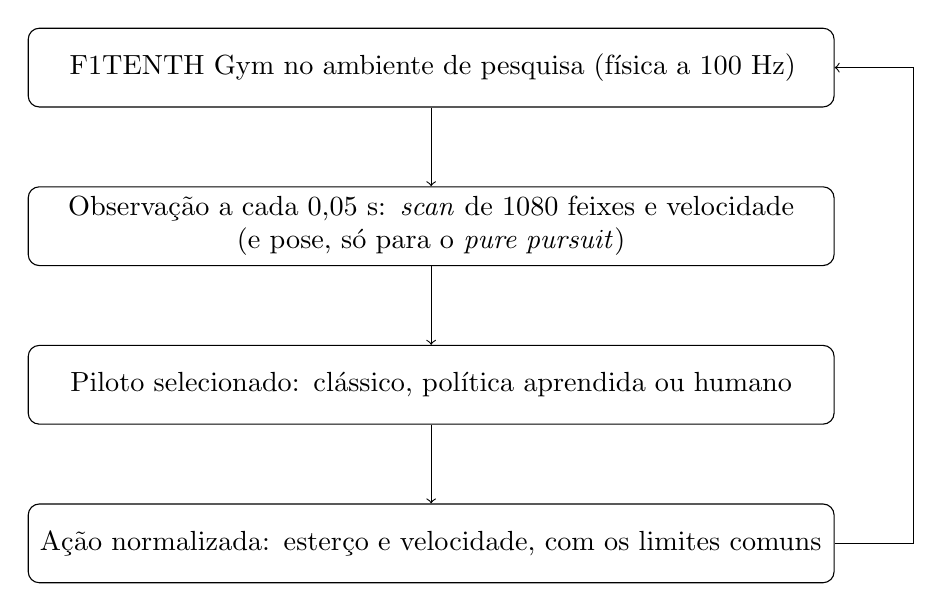
\begin{tikzpicture}[node distance=1cm, every node/.style={align=center},
box/.style={draw, rounded corners, text width=10cm, minimum height=1cm}]
\node[box] (gym) {F1TENTH Gym no ambiente de pesquisa (física a 100~Hz)};
\node[box, below=of gym] (sensor) {Observação a cada 0,05~s: \textit{scan} de 1080 feixes e velocidade\\(e pose, só para o \textit{pure pursuit})};
\node[box, below=of sensor] (control) {Piloto selecionado: clássico, política aprendida ou humano};
\node[box, below=of control] (drive) {Ação normalizada: esterço e velocidade, com os limites comuns};
\draw[->] (gym) -- (sensor);
\draw[->] (sensor) -- (control);
\draw[->] (control) -- (drive);
\draw[->] (drive.east) -- ++(1,0) |- (gym.east);
\end{tikzpicture}
\caption{Laço de controle medido no ambiente de pesquisa. Um piloto por vez
recebe a observação e devolve a ação, sob o mesmo avaliador.}
\label{fig:software_arch}
\end{figure}

\section{Navegação reativa no simulador}

\subsection{Disparity Extender}

O Disparity Extender é o método divulgado por Otterness
\cite{Otterness2019Disparity}, descrito na Seção~\ref{sec:arte-classico}. Esta
subseção descreve o nó ROS2 original do repositório. O objeto medido no comparativo é o
seu porte para o ambiente de pesquisa, sem ROS, descrito na
Seção~\ref{sec:prop-portes}, que diverge do nó em pontos ali declarados.

O arquivo \path{src/wall_follow/wall_follow/wall_follow.py} define a classe
\texttt{WallFollowHybrid}. A implementação atual usa Disparity Extender, não
o antigo controlador de distância lateral com a classe \texttt{WallFollow}.
O nome do pacote foi preservado para compatibilidade com as ferramentas do projeto.

O processamento, resumido na Figura~\ref{fig:wall_follow_arch}, limita os alcances a 5~m e aplica um filtro de média uniforme
de cinco amostras. Uma região de proteção é removida ao redor do obstáculo
frontal mais próximo. Diferenças de alcance superiores a 0,3~m identificam
bordas; o algoritmo estende o menor alcance para cobrir a largura considerada
do veículo, reduzindo a possibilidade de escolher uma passagem estreita.
Em seguida, seleciona uma sequência de feixes livres e um alvo dentro dela.
O esterçamento é limitado e suavizado; a velocidade depende do espaço frontal
e da curvatura solicitada. Esses valores são parâmetros da implementação e
não demonstram, por si só, segurança ou desempenho em todas as pistas.

\begin{figure}[htb]
\centering
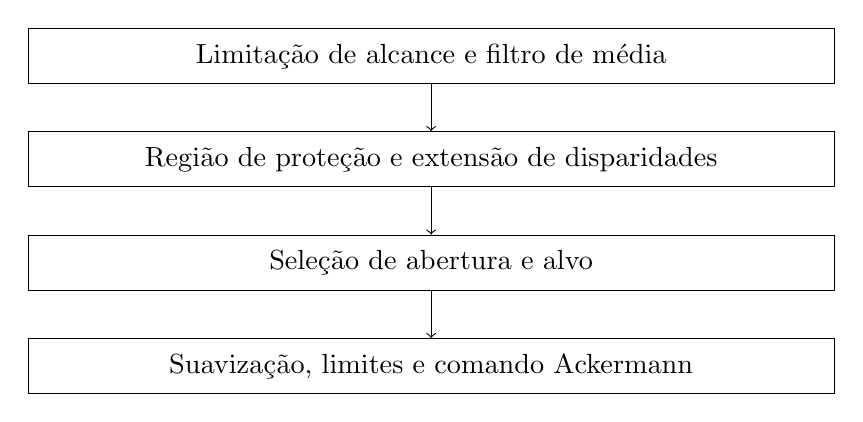
\begin{tikzpicture}[node distance=0.6cm,
box/.style={draw, text width=10cm, align=center, minimum height=0.7cm}]
\node[box] (a) {Limitação de alcance e filtro de média};
\node[box, below=of a] (b) {Região de proteção e extensão de disparidades};
\node[box, below=of b] (c) {Seleção de abertura e alvo};
\node[box, below=of c] (d) {Suavização, limites e comando Ackermann};
\draw[->] (a)--(b); \draw[->] (b)--(c); \draw[->] (c)--(d);
\end{tikzpicture}
\caption{Processamento reativo do pacote \texttt{wall\_follow} no simulador.}
\label{fig:wall_follow_arch}\label{fig:wall_follow_flow}
\end{figure}

\subsection{Seguimento de gap}

Também aqui a descrição é a do nó ROS2 original, com seus temporizadores e prazos
de validade. O comparativo mede o porte sem ROS da Seção~\ref{sec:prop-portes},
em que a sincronização por temporizadores desaparece: a política é chamada uma
vez por passo de controle.

A classe \texttt{ThreadedGapFollower} está implementada em
\path{src/gap_follow/gap_follow/gap_follow.py}. Apesar desse nome histórico, sua execução atual
usa dois temporizadores ROS2 configurados para 100~Hz e o executor padrão de
\texttt{rclpy.spin}. Não existem filas de scans e comandos nem threads de
processamento criadas pelo nó. Os grupos de callbacks são reentrantes, mas
isso não transforma o executor padrão em um executor paralelo.

A Figura~\ref{fig:gap_follow_arch} resume esse fluxo. O callback de scan guarda a
observação mais recente. Um temporizador aplica
filtro de mediana, converte os pontos para coordenadas cartesianas, identifica
descontinuidades e escolhe uma abertura. O estado intermediário é armazenado
em \texttt{latest\_scan\_data}. O outro temporizador calcula os comandos PID
de direção e velocidade. A frequência configurada não implica que todos os
ciclos cumpram o prazo; essa propriedade exige medição durante a execução.

\begin{figure}[htb]
\centering
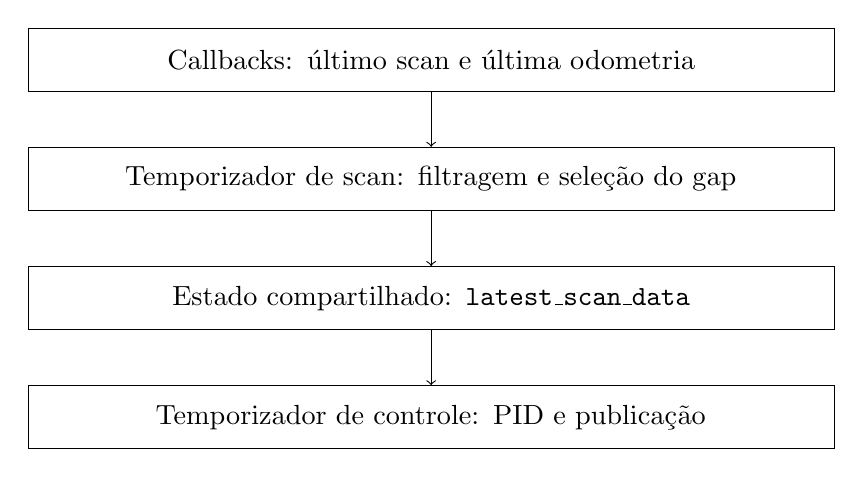
\begin{tikzpicture}[node distance=0.7cm,
box/.style={draw, text width=10cm, align=center, minimum height=0.8cm}]
\node[box] (a) {Callbacks: último scan e última odometria};
\node[box, below=of a] (b) {Temporizador de scan: filtragem e seleção do gap};
\node[box, below=of b] (c) {Estado compartilhado: \texttt{latest\_scan\_data}};
\node[box, below=of c] (d) {Temporizador de controle: PID e publicação};
\draw[->] (a)--(b); \draw[->] (b)--(c); \draw[->] (c)--(d);
\end{tikzpicture}
\caption{Fluxo do seguidor de gap, executado por callbacks e temporizadores.}
\label{fig:gap_follow_arch}\label{fig:gap_follow_flow}
\end{figure}

As coordenadas são obtidas por $x_i=r_i\cos\theta_i$ e
$y_i=r_i\sin\theta_i$, com $\theta_i=\theta_{min}+i\Delta\theta$.
A distância entre pontos consecutivos identifica candidatos a abertura; a
seleção combina sua largura e posição. A odometria fornece a velocidade usada
pelo controlador. As saturações limitam a saída do PID e o mecanismo de
anti-windup reduz o acúmulo integral durante a saturação.

A configuração usa o formato ROS2 \texttt{ros\_\_parameters}. O tópico de
odometria padrão é \texttt{/ego\_racecar/odom}. O tempo usado por padrão é o
do sistema, pois a ponte não publica \texttt{/clock}. Scans e odometria têm
prazo de validade de 0,5~s; ausência ou expiração invalida o processamento e
produz um comando de parada. Esse mecanismo evita perpetuar comandos a partir
de uma observação antiga.

\section{Controladores reativos portados para o ambiente de pesquisa}\label{sec:prop-portes}

O Disparity Extender e o seguidor de gap entram no comparativo como políticas do
ambiente de pesquisa (\texttt{research/}), escritas em Python sem ROS. Cada porte
é uma política que recebe o \textit{scan} bruto de 1080 feixes (\texttt{scan\_raw})
e a velocidade longitudinal, e devolve a ação normalizada pelos mesmos limites das
demais políticas. Não usam pose, mapa nem linha de corrida, o que os separa do
\textit{pure pursuit} do E1. O ângulo de cada feixe segue a convenção do
simulador, com o primeiro feixe à direita e o último à esquerda, de modo que uma
abertura à esquerda produz esterço positivo.

\textbf{Pipelines.} O porte do Disparity Extender preserva o processamento da
Figura~\ref{fig:wall_follow_arch}: limite de alcance, filtro de média, região de
proteção ao redor do obstáculo frontal, extensão de disparidades pela largura do
carro, seleção de abertura e alvo, esterço limitado e suavizado, e velocidade
decidida pelo espaço frontal e pela curvatura pedida. O porte do seguidor de gap
preserva o filtro de mediana, a conversão para coordenadas cartesianas, a
identificação de descontinuidades maiores que um limiar de profundidade, a
pontuação das aberturas por distância e largura, o PID de esterço e a regra de
velocidade, com a opção de usar o PID de velocidade do nó ou o alvo direto.

\textbf{O que muda em relação aos nós.} Quatro adaptações são comuns. Primeiro, as
velocidades originais, próprias de um veículo real lento, são reescaladas para o
envelope de 1 a 8~m/s do ambiente, e o teto de velocidade de cada porte é um
parâmetro, mantendo-se a forma da regra de velocidade de cada nó. Segundo, o
esterço é sempre cortado na saturação comum de $\pm 0{,}4189$~rad, que o ambiente
impõe a todos os pilotos; o nó do seguidor de gap saturava em valor maior.
Terceiro, os PIDs avançam com o passo de controle de 0,05~s em tempo de simulação,
e não com o relógio nem com os 100~Hz fixos do nó. Quarto, o comando de parar do
original não existe, porque a velocidade mínima do ambiente é 1~m/s: onde o nó
mandava parar, o porte devolve esterço nulo e velocidade mínima.

\textbf{Correção da extensão de disparidades.} O porte do Disparity Extender
diverge do nó em um ponto de lógica. O nó estendia o alcance curto sobre o
próprio obstáculo, o que quase não alterava o \textit{scan}. O porte estende o
lado distante de cada borda, o vão que parece livre, pela largura do carro, com as
disparidades detectadas no \textit{scan} original, pois detectá-las sobre o
\textit{scan} já estendido propagaria o alcance curto por todo o vetor
(\texttt{SPEC-RCT-09}).

\textbf{Varredura de parâmetros e configuração congelada.} Os valores dos
parâmetros dos nós foram escolhidos para outro regime de velocidade, e portanto
cada porte passa por uma varredura curta em grade, no estilo da varredura do E1,
com no máximo 24 combinações por grade; o seguidor de gap, que não completou volta
na grade oficial, teve também uma grade ampliada, num total de 48 combinações. Para o Disparity Extender, a grade varia o teto de
velocidade, a largura efetiva do carro, o raio da bolha de segurança e o ganho de
esterço; para o seguidor de gap, o teto de velocidade, a profundidade máxima de
descontinuidade, o ganho proporcional do esterço e o modo de velocidade. O
critério de escolha é fixado antes de qualquer medição: cada combinação corre
uma volta em cada uma de três \textit{seeds} de sonda (2000, 2001 e 2002), com
randomização e largada na linha de corrida, e vence a que tiver mais voltas
completas; o empate se desfaz pela menor mediana do tempo de volta, e um novo
empate pela menor taxa média de esterço. Se nenhuma combinação completar uma
volta, vence a de maior progresso médio. As \textit{seeds} de sonda são
distintas das de avaliação (1000 a 1004), para que a configuração escolhida não
seja a que melhor decorou as largadas medidas depois. A configuração vencedora é
gravada em um arquivo versionado, com a grade, o resultado de cada combinação e o
critério, e a avaliação lê apenas esse arquivo. Um desempenho fraco da
configuração congelada é, portanto, um resultado do método, e não motivo para
nova busca.

\section{Interface de pilotagem humana}\label{sec:prop-humano}

O piloto humano conduz o mesmo veículo simulado, no mesmo ambiente e sob o mesmo
avaliador das políticas. A interface é um pacote do ambiente de pesquisa, e esta
seção descreve o seu contrato, não a sua implementação.

\textbf{Entrada.} O piloto usa um \textit{joystick}. O analógico esquerdo, na
horizontal, esterça, e mover para a esquerda produz esterço positivo, que vira o
carro à esquerda. O gatilho direito controla a velocidade: solto, o carro anda a
1~m/s; apertado até o fundo, a 8~m/s. O carro nunca para nem dá ré. O esterço tem
uma zona morta pequena, para que o analógico em repouso não mova o carro, e os
eixos são calibrados por \textit{joystick}, com índice, valor em repouso, valor
no fundo e inversão gravados em um arquivo de calibração.

\textbf{Mesmos limites e atraso.} A ação do humano passa pela mesma normalização
das políticas: esterço máximo de $\pm 0{,}4189$~rad, velocidade entre 1 e 8~m/s,
atraso de esterço de dois passos (100~ms) e passo de controle de 0,05~s. Assim,
nenhuma diferença de resultado entre humano e política vem de um limite de
atuação mais folgado para um dos lados.

\textbf{Tempo real.} A cada passo, a interface desenha o estado, lê o
\textit{joystick} e segura o passo até o prazo absoluto de 0,05~s de relógio,
em vez de dormir um intervalo fixo, de modo que o atraso de um passo não se
acumula nos seguintes. O atraso de cada passo é registrado (média, percentil 95,
percentil 99, máximo e número de passos que passaram do prazo), para que
um eventual passo lento seja declarado e não oculto. Antes da primeira chamada de
cada sessão há uma contagem regressiva de 3~s.

\textbf{Vistas e painel.} Há duas vistas. Na vista da \textit{pista inteira}, o
mapa da pista é mostrado de cima, com o carro desenhado na pose atual. Na vista
\textit{só LiDAR}, aparecem apenas os pontos do \textit{scan} atual no referencial
do carro, com o carro fixo no centro apontando para cima, sem mapa e sem rastro,
dentro de um alcance fixo. A segunda vista dá ao humano informação equivalente à
da política: o \textit{scan} atual, dentro de um alcance fixo, e a velocidade no
painel. Nas duas, um painel mostra a velocidade, o tempo da volta atual e
o da última, e o estágio (``Treino mm:ss'' ou ``Sessão $k$ · volta $j$/5'').

\textbf{Gravação.} Para cada piloto e vista, a interface produz um registro no
mesmo formato dos pilotos automáticos: relatório de avaliação, dados passo a
passo das sessões que contam, dados do treino, atraso por passo, calibração do
\textit{joystick}, versão do código e \textit{hash} do protocolo. O piloto é
identificado por um código anônimo, e nenhum nome aparece nos dados. O protocolo
que usa essa interface é descrito na Seção~\ref{sec:val-humano}.

\section{Execução das políticas aprendidas}

No comparativo, as políticas aprendidas são executadas no próprio ambiente de
pesquisa: o avaliador carrega o ponto de verificação aprovado de cada etapa e
chama a rede a cada passo de controle, sem retreino e sem exportação
(Seção~\ref{sec:res-cmp-proveniencia}). A política recebe o \textit{scan} e a
informação proprioceptiva do passo, e a sua ação passa pelos mesmos limites dos
demais pilotos.

A memória recorrente separa a ação base da ação após a saturação. Essa
distinção é necessária para o residual do estágio E3, pois limitar uma
solicitação altera o histórico de atuação observado no passo seguinte.

\section{Simulador e reprodução}

O ambiente de pesquisa executa a física do F1TENTH Gym a 100~Hz e o controle a
20~Hz, com passo de 0,05~s e atraso de esterço de dois passos. A colisão é
detectada pelo avaliador, e a randomização de atrito, de posição de largada e de
ruído do LiDAR é sorteada por semente, de modo que dois pilotos avaliados na
mesma semente enfrentam as mesmas condições. O incremento angular do
\textit{scan} é a abertura total dividida por $N-1$, coerente com os extremos
inclusivos dos $N$ feixes do simulador.

Cada execução é reproduzida por um comando do ambiente de pesquisa, que lê a
configuração gravada e grava, ao lado dos resultados, a versão do código, o
\textit{hash} dos critérios e o estado da árvore de trabalho. Os comandos
completos estão no README do ambiente de pesquisa, mantendo os procedimentos
operacionais junto ao código.

A comparação dos controladores deve distinguir algoritmo, configuração,
versão e ambiente. A existência de um controlador no repositório não comprova
ausência de colisão nem conclusão de volta. Essas propriedades
são avaliadas pelos procedimentos e artefatos descritos no capítulo seguinte.

\chapter{Metodologia de Validação Experimental}\label{cap:metodologia}

Os capítulos anteriores descrevem o que foi construído: a pilha de
software, o simulador e as políticas de controle. Este capítulo descreve o
aparato que decide se um número produzido por esse conjunto pode ser reportado.
São coisas diferentes, e a distinção é o assunto do capítulo.

A prática corrente em aprendizado por reforço aplicado a corrida autônoma
reporta uma métrica agregada --- taxa de conclusão de voltas, tempo de volta,
distância percorrida --- acompanhada de uma descrição do treino
\cite{Betz2022Survey}. O leitor recebe o valor e a receita, e a reprodutibilidade
é tratada como consequência de ambos. O que se argumenta aqui, com base em
falhas medidas e não em princípio geral, é que valor e receita são insuficientes:
entre o experimento e o número existe um conjunto de decisões --- definição do
evento que a métrica conta, protocolo de avaliação, composição da política
avaliada, critério de aceite, momento em que o critério foi fixado --- que não
aparece na receita e que altera o número em magnitude comparável à das diferenças
que o trabalho pretende demonstrar.

Todos os resultados discutidos neste capítulo foram obtidos \textbf{em
simulação}, no ambiente \texttt{f110\_gym} \cite{OKelly2020F1TENTH}. A simulação
é uma escolha de escopo do trabalho, que compara pilotos dentro de um mesmo
simulador e sob um mesmo avaliador, e não uma limitação contornada: o que a
validação descrita garante é que o número comparado entre os pilotos mede o que
o texto diz que mede.

O capítulo está organizado em torno de um argumento único, exposto em sete
partes. A Seção~\ref{sec:val-problema} apresenta quatro falhas reais do projeto
que motivam tudo o que vem depois. A Seção~\ref{sec:val-contrato} descreve o contrato
numérico com identificador, que é a forma escolhida para impedir que uma decisão
de projeto vire folclore. A Seção~\ref{sec:val-congelado} trata de congelar
critérios antes da medição, e de tornar a proveniência do resultado parte do
veredito. A Seção~\ref{sec:val-estatistica} trata da decisão estatística e do
escalonamento automático de amostra. A
Seção~\ref{sec:val-humano} aplica o aparato ao comparativo, com o protocolo
comum, os pilotos humanos e as métricas novas. A Seção~\ref{sec:val-camadas}
descreve as cinco camadas de verificação. A
Seção~\ref{sec:val-limitacoes} declara o que este aparato não cobre.

\section{O problema: um número medido não é um resultado}\label{sec:val-problema}

Quatro episódios do desenvolvimento ilustram o problema melhor do que uma
formulação abstrata. Os quatro produziram números plausíveis, internamente
consistentes e reprodutíveis --- no sentido de que reexecutar o mesmo comando
devolvia o mesmo valor --- e os quatro estavam errados por motivos distintos.

\subsection{O detector de colisão do simulador não detecta
colisão}\label{sec:val-colisao}

O primeiro caso é o mais básico dos quatro, porque não corrompe um número: corrompe
a definição do evento que todos os números contam. Taxa de conclusão de voltas,
tempo de volta e distância percorrida são todos condicionados a ``o veículo não
bateu''. Quem decide isso, no \texttt{f110\_gym}, é uma rotina
(\texttt{check\_ttc\_jit}) que estima tempo até a colisão a partir do próprio scan
do LiDAR. Auditada contra verdade de campo --- o retângulo do veículo amostrado
sobre o mesmo grid de ocupação que o simulador carregou ---, ela apresentou seis
defeitos, todos reproduzidos em simulação e registrados em \texttt{SPEC-COL}.

Três deles bastam para a leitura. O primeiro é geométrico: a rotina dispara dentro
de uma \textbf{faixa} de folga, e não num semiplano; quem atravessa a faixa inteira
num único passo de física não é detectado nem naquele passo nem em nenhum outro
depois, porque a partir dali a folga é negativa e a condição reprova. O segundo é
uma guarda de velocidade (\texttt{if vel != 0.0}) no topo da rotina: veículo parado
encostado no muro não colide. O terceiro é o mais destrutivo, porque atinge o estado
\textbf{físico} e não apenas o que se reporta: a rotina zera as componentes de
estado a partir da quarta, e a quinta é o \textit{yaw}. Toda batida teleporta a
orientação do veículo para 0~rad. Medido: 3,763~rad $\rightarrow$ 0,000.

O que transforma isso de curiosidade em erro de medição é a geometria destes mapas.
As paredes são uma fita de \textbf{9 a 38~cm} com espaço livre atrás, em 40 de 40
seções amostradas nas cinco pistas, enquanto a 8~m/s o veículo percorre 8~cm por
passo de física. Espessura de parede e passo de integração são da mesma ordem: a
travessia num único passo não é o caso patológico, é o caso comum.

O efeito composto foi medido na ponte ROS2, que agravava o quadro por não ler a
chave \texttt{collisions} da observação devolvida pelo simulador --- a marca de
colisão nascia falsa e morria falsa, e não havia tópico que a publicasse. Largando o
veículo a 1,1~m do muro, a 2~m/s, contra ele: o carro atravessou a parede em
$(-44{,}24;\ 3{,}32)$, teve o \textit{heading} zerado no impacto e seguiu dirigindo
sozinho na área externa, parando em
$(-30{,}14;\ 3{,}31)$ --- 14~m adiante do ponto de impacto, fora do circuito. Nada
nessa execução acusou colisão. Uma volta assim é contada como completa, e a
distância percorrida segue sendo integrada do lado de fora da pista.

A correção está em \texttt{SPEC-COL-01} a \texttt{SPEC-COL-06} e redefine o evento
em vez de ajustar o detector: colidiu passa a ser existir ponto do retângulo do
veículo sobre célula ocupada \textbf{ou} a marca do simulador ter acendido; a
checagem é do \textbf{segmento} entre a pose anterior e a atual, e não dos extremos,
que é o que impede atravessar uma parede de 9~cm com as duas poses em espaço livre;
sair dos limites do mapa conta como colisão; o grid consultado é o \textbf{mesmo}
que o simulador usou para gerar o scan, de modo que a geometria da colisão não possa
discordar da geometria que o LiDAR enxerga; e a pose reportada no passo da colisão
preserva o último \textit{heading} válido.

Uma restrição de engenharia acompanha a correção e é parte dela. Ela vive num
invólucro, e o \texttt{f110\_gym} incorporado ao repositório permanece no commit
fixado (\texttt{SPEC-COL-07}), com teste que falha se alguém o alterar. O que o
simulador executa continua sendo o código original, e o scan do ambiente de
pesquisa segue idêntico ao que o mesmo simulador produz no \textit{workspace} ROS2
do repositório --- uma paridade herdada da fase com veículo e ainda verificada
pela Camada~C (Seção~\ref{sec:val-camadas}). Corrigir o critério de colisão sem tocar no simulador é o que
permite as duas coisas ao mesmo tempo.

\subsection{Vazamento de estado entre episódios}

A política da segunda etapa do trabalho (E2, aprendizado por imitação) guarda o
scan do instante anterior e os últimos comandos de esterço e velocidade
(\texttt{scan\_prev}, \texttt{prev\_steer}, \texttt{prev\_speed}) numa closure, e
não expõe método de reinicialização. O avaliador construía \textit{uma} instância
da política e a reutilizava para todos os episódios da avaliação.

A consequência é que o episódio seguinte largava com o scan do instante da
colisão anterior. Do ponto de vista da rede, isso é um deslocamento entre a pose
colidida e a nova largada --- um par de quadros que não existe em lugar nenhum do
treino, onde todo primeiro quadro após o \textit{reset} tem
\texttt{scan\_prev == scan} por construção.

O efeito não é um viés pequeno: é binário. Com duas sementes por pista no
conjunto de generalização, uma pista saía 0/2 ou 6/6, e nunca no meio. E ele se
disfarça de má generalização, que é exatamente a hipótese que um pesquisador
formularia primeiro diante desse padrão. \textbf{Foram oito execuções do E2
reprovadas assim antes de a causa aparecer.} O agravante metodológico é que o
controle não era afetado: o especialista da primeira etapa (E1, \textit{pure
pursuit}) não guarda estado, e por isso era imune --- o que fazia o contraste
entre especialista e rede parecer mérito do especialista.

A correção é uma linha de protocolo, hoje registrada como
\texttt{SPEC-EVAL-01}: cada semente recebe uma política \textbf{recém-construída};
a função de fábrica é chamada uma vez por semente, nunca uma vez por avaliação.
Nenhum estado atravessa a fronteira de episódio.

\subsection{Duas cópias da mesma composição de política}\label{sec:val-duascopias}

A terceira etapa (E3) é um resíduo de aprendizado por reforço somado à saída da
rede do E2. Compor as duas exige montar um vetor de ganhos, aplicar a saída de
uma sobre a da outra e clipar o resultado. Durante um período existiram
\textit{duas} implementações dessa composição: uma usada pelo treino, outra pela
reavaliação.

Elas divergiam num detalhe que qualquer revisor classificaria como inofensivo: o
vetor de ganhos era \texttt{float64} numa e \texttt{float32} na outra. Medido no
\textit{mesmo} ponto de verificação, com as \textit{mesmas} sementes, o resultado
foi \textbf{97,56\%} (40/41 voltas, 1 colisão) contra \textbf{91,43\%} (32/35
voltas, 3 colisões). A diferença induzida na ação é da ordem de $10^{-7}$.

O achado não é que uma das implementações estivesse errada --- nenhuma estava. É
que o sistema amplifica ruído de ponto flutuante ao longo de milhares de passos
de controle. Isso foi medido diretamente, perturbando o vetor de ganhos por
epsilons crescentes e reavaliando o mesmo ponto de verificação com as mesmas
cinco sementes em Spielberg:

\begin{table}[h]
    \centering
    \begin{tabular}{|c|c|c|}
        \hline
        \textbf{$\varepsilon$} & \textbf{E3 (resíduo)} & \textbf{E2 (rede base)} \\
        \hline
        0          & 97,56\%         & 97,56\%         \\
        \hline
        $10^{-12}$ & 93,75\%         & 97,56\%         \\
        \hline
        $10^{-9}$  & 94,29\%         & 97,56\%         \\
        \hline
        $10^{-7}$  & 94,59\%         & 97,56\%         \\
        \hline
        $10^{-5}$  & 97,56\%         & 97,56\%         \\
        \hline
        \textbf{amplitude} & \textbf{0,0381} & \textbf{0,0000} \\
        \hline
    \end{tabular}
    \caption{Completion sob perturbação do vetor de ganhos, mesmo ponto de
    verificação e mesmas sementes (\texttt{SPEC-EVAL-02})}
    \label{tab:val_sensibilidade}
\end{table}

A leitura da Tabela~\ref{tab:val_sensibilidade} tem duas partes. A perturbação
não tem tendência nem ordem: ela reembaralha \textit{qual} episódio bate, não
desloca o resultado numa direção. E o contraste entre as etapas é o achado
central: a política do E2 é \textit{insensível} a perturbações cobrindo sete
ordens de grandeza, enquanto a do E3 espalha 3,8 pontos percentuais. Isso é
coerente com o que as duas fazem --- o resíduo dirige no limite (53,7~s contra
58,8~s da rede base naquela medição), onde uma diferença mínima decide quem bate.

A consequência metodológica está registrada em \texttt{SPEC-EVAL-02} e é
retomada na Seção~\ref{sec:val-limitacoes}: a composição da política avaliada,
\textbf{inclusive tipos numéricos e ordem de operações}, é parte do protocolo, e
não detalhe de implementação. Hoje existe uma única função que monta a
composição, usada pelo treino e pela reavaliação.

\subsection{Três valores para a mesma medição}

A quarta falha não é de código: é de documentação. Três valores diferentes para
a \textit{mesma} medição de distância percorrida numa verificação em tempo real da política ---
337~m, 428~m e 552,7~m --- conviveram simultaneamente no repositório, em
documentos distintos, cada um apresentado como o resultado vigente. Pior: um
deles citava como evidência um arquivo que o contradizia.

Nenhum teste falhava, porque nenhum teste lê prosa. Nenhuma execução divergia,
porque o código estava certo. O defeito vivia inteiramente na camada que o leitor
consulta, e a origem de um dos valores foi posteriormente rastreada: a
verificação não encerrava os nós ROS2 de execuções anteriores, e a leitura de 552~m
saiu com um nó de 1~h~18~min publicando comandos ao lado do nó novo --- duas
políticas comandando o mesmo veículo simulado.

\subsection{O que os quatro casos têm em comum}

Nos quatro, reexecutar o comando devolvia o mesmo número. Nos quatro, o número
estava errado. E nos quatro a distância entre o valor errado e o valor correto é da
mesma ordem de grandeza das diferenças que o trabalho pretende demonstrar --- uma
volta contada como completa depois de o veículo sair do circuito, 6 pontos de
\textit{completion}, uma pista inteira zerada, 200~m de distância percorrida.

Isso delimita o que a validação precisa cobrir. Não basta verificar que o
programa roda, nem que ele é determinístico: é preciso verificar que o evento
contado pela métrica corresponde ao que de fato acontece no mundo simulado, que o
protocolo de avaliação não vaza estado, que existe uma única definição executável
do objeto avaliado, que o critério de aceite foi fixado antes da medição, que o
número citado no texto corresponde a um artefato em disco. Cada uma dessas verificações é uma camada, e é
delas que trata o restante do capítulo. A verificação formal de propriedades de
segurança de controladores neurais \cite{Ivanov2020Verifying} e a busca ativa por
cenários de falha \cite{Bak2021Stress} atacam um problema adjacente e
complementar; o que se discute aqui é anterior a ambos, porque diz respeito à
confiabilidade do próprio número que se pretende verificar.

\section{Contrato numérico com identificador}\label{sec:val-contrato}

O primeiro mecanismo é um documento único, \texttt{SPEC.md}, em que cada decisão
numérica do ambiente de pesquisa é escrita como uma asserção testável com
identificador estável. Na versão vigente, contada em outubro de 2026, são
\textbf{118 asserções}, distribuídas em 20 famílias temáticas, com
identificadores da forma \texttt{SPEC-<FAMÍLIA>-<NN>}.

\subsection{O que uma asserção contém}

Uma asserção não é um comentário: ela fixa um valor, uma unidade e um
comportamento observável. \texttt{SPEC-OBS-01}, por exemplo, estabelece que o
scan de 1080 feixes é reduzido a 60 por média de janelas de 18, e registra a
razão --- $1080/60 = 18$ é exato, a média preserva melhor o obstáculo mais
próximo do que a decimação, e 64 feixes dariam janela fracionária.
\texttt{SPEC-ENV-01} fixa a física em 100~Hz e o controle em 20~Hz, com cinco
passos de simulação por passo de controle. \texttt{SPEC-ACT-02} fixa
$\delta = a_0 \cdot 0{,}4189$~rad, o limite de esterço do modelo
\textit{single-track}.

Além do valor, a maior parte das asserções registra \textbf{a falha que a
originou}. Essa é a diferença entre um documento de especificação e este: quase
todo item nasceu de um defeito medido, e o registro da medição viaja junto com a
regra. \texttt{SPEC-FRE-04} é um exemplo instrutivo. A projeção de Frenet
usada para medir progresso levantava exceção sempre que o deslocamento
longitudinal num passo excedia 2~m, sob a premissa de que todo salto grande fosse
teleporte ou defeito de projeção. A premissa é falsa: Spielberg tem uma forquilha
de raio 0,84~m, menor que a meia-largura de 1,10~m da pista, e no centro de
curvatura todas as normais da linha central se encontram, deixando o pé da
projeção indefinido. Medido: carro a 0,25~m desse centro, \textit{dentro} da
pista, a 4,78~m/s, sem colisão, com salto de 2,39~m em um passo de 50~ms. Nem
levantar nem aceitar em silêncio servem --- levantar mata um treino de doze
minutos por geometria legítima; aceitar dá $+0{,}239$ de recompensa contra
$+0{,}04$ de um passo normal, num ponto \textit{fixo} da pista, que um agente
aprende a explorar. A regra vigente limita o deslocamento a 2~m e \textit{conta}
o evento, com o viés resultante demonstrado conservador. Os três parágrafos que
sustentam essa escolha estão no próprio item do contrato, não numa discussão
perdida em histórico de versão.

\subsection{O teste que impede o contrato de virar prosa morta}

Um documento de especificação sem execução apodrece: alguém acrescenta uma
asserção, ninguém escreve o teste, e o documento passa a descrever um sistema que
não existe. A defesa é a Camada~A, um teste que varre o \texttt{SPEC.md}, extrai
o conjunto de identificadores declarados e o conjunto de identificadores citados
nos arquivos de teste, e \textit{falha} se a diferença for não vazia. A mensagem
de falha é deliberadamente estreita: ou se escreve o teste que falta, ou se
remove o item do contrato.

Há um segundo teste na direção oposta: nenhum teste pode citar um identificador
que não exista no contrato. Sem ele, um erro de digitação numa docstring
satisfaria a cobertura sem verificar coisa alguma.

A ressalva honesta é que essa checagem é \textbf{por ocorrência textual}: ela
garante que o identificador foi citado no arquivo de teste, não que o teste
exerça o que a asserção afirma. A limitação é discutida em detalhe na
Seção~\ref{sec:val-limitacoes}.

\section{Critérios congelados antes da medição}\label{sec:val-congelado}

A segunda família de mecanismos ataca um modo de falha que nenhum teste unitário
alcança: mover a trave depois de ver o número. Ele não exige má-fé --- basta que
o limiar viva num arquivo de configuração editável e que a avaliação possa ser
reexecutada sobre um relatório antigo.

\subsection{Proveniência como veredito, não como metadado}

Duas asserções do contrato não julgam a política: julgam a \textit{medição}. Um
número correto obtido de forma não defensável não é reportável, e o lugar de
dizer isso é o próprio veredito do portão.

\texttt{SPEC-PROV-01} determina que o \texttt{config.yaml} de cada execução
congele, no momento em que a execução nasce, o conjunto de limiares em vigor e
uma assinatura deles (\texttt{gate\_hash}). Se, na hora de avaliar, os limiares
em vigor não baterem com os congelados, o veredito é \texttt{INVALIDO} --- nem
\texttt{PASS} nem \texttt{FAIL}. A motivação está registrada: o contrato afirmava
desde o início que as faixas eram fixadas antes de treinar, e não existia nenhum
artefato capaz de provar isso depois, porque nenhum limiar era gravado na
execução. Era possível editar a configuração e reexecutar a avaliação sobre um
relatório antigo sem que nada denunciasse.

\texttt{SPEC-PROV-02} determina que um \texttt{PASS} obtido com a árvore de
trabalho suja seja rebaixado a \texttt{PASS-NAO-REPRODUZIVEL}. Com mudanças não
commitadas, o identificador de commit registrado não descreve o código que
produziu o resultado --- e esse campo era gravado e nunca lido por ninguém. O
caso que forçou a regra é revelador do quanto o mecanismo precisa ser
automático: uma ação pré-declarada do laço automático disparava a recalibração do
ruído de coleta, e o laudo era gravado num arquivo versionado. A árvore sujava no
meio da execução, e a tentativa seguinte nascia marcada como suja. A quinta
tentativa do E2 passou nos quatro critérios e saiu
\texttt{PASS-NAO-REPRODUZIVEL}: o laço invalidou, pela própria regra, o resultado
que ele mesmo produziu. A correção (\texttt{SPEC-DART-05}) move o laudo novo para
o diretório da execução e para um cache fora do controle de versão; o laudo
citado pelo trabalho passa a ser somente de leitura, atualizado por ato humano
explícito.

\texttt{SPEC-PROV-03} exige que a configuração grave o dispositivo de treino
\textit{resolvido}, nunca o literal \texttt{"auto"}. O dispositivo muda os pesos:
kernels diferentes e ordem de redução diferente produzem resultado diferente com
a mesma semente --- medido, uma divergência de $1{,}34 \times 10^{-2}$ nos pesos
entre CPU e GPU. Sem o campo, uma execução em CPU e outra em GPU sairiam com
configuração byte a byte idêntica e pontos de verificação distintos, e a
configuração é exatamente o artefato que deveria permitir refazer a execução.
Pedir GPU numa máquina sem GPU \textbf{levanta exceção}; cair para CPU em
silêncio devolveria outro experimento sob a mesma configuração.

O valor prático dessas três regras aparece quando o resultado sobrevive a elas. O
tempo do especialista, denominador de todos os critérios de E2 e E3, foi
remedido com a árvore limpa e reproduziu o valor anterior até o último dígito
($T_{pp} = 58{,}99999999994634$~s), inclusive entre arquiteturas distintas
(arm64 e x86\_64). Essa coincidência não era garantida --- aritmética de ponto
flutuante entre ISAs diferentes não precisa concordar bit a bit --- e é o que
autoriza comparar as tabelas novas com as antigas.

\subsection{Ações pré-declaradas por critério}

Congelar o limiar não basta se a escolha do próximo hiperparâmetro for feita
olhando o resultado. O mecanismo correspondente é uma tabela de ações
pré-declaradas, indexada pelo \textit{critério} que reprovou --- não pela etapa
--- e percorrida em ordem fixa pelo laço automático.

A indexação por critério, e não por etapa, foi ela própria uma correção. Na
versão anterior, o laço lia apenas o veredito e descartava a lista de critérios.
Com o critério de generalização reprovando, ele aplicava, em ordem, as cinco
ações declaradas ``do E2'', todas sobre o conjunto de dados de uma única pista, e
nenhuma capaz de mover generalização --- cinco tentativas de aproximadamente uma
hora, garantidamente inúteis. A regra correspondente
(\texttt{SPEC-LOOP-02}) exige que o ajuste venha da lista pré-declarada
\textbf{do critério que reprovou}, na ordem em que os critérios aparecem no
relatório do portão.

Três asserções complementares fecham modos de falha vizinhos.
\texttt{SPEC-LOOP-03} exige que a tabela executável e a tabela textual exibida no
diagnóstico cubram os mesmos critérios com o mesmo número de ações --- quando
eram indexadas de formas diferentes, o diagnóstico prometia uma ordem e o laço
executava outra. \texttt{SPEC-LOOP-07} exige que toda chave declarada seja
parâmetro que a etapa \textbf{de fato consome}, e nasceu de dois casos reais:
\texttt{wall\_w} e \texttt{mu\_std} estavam declarados, existiam nas estruturas
de configuração, e a função construtora do ambiente não os repassava. Um ajuste
que a etapa ignora produz uma execução idêntica à anterior e consome uma
tentativa --- e \texttt{mu\_std} era a \textit{primeira} ação de dois dos quatro
critérios do E3. \texttt{SPEC-LOOP-06} determina que falha das camadas de teste
ou de invariantes não consuma tentativa: é defeito de código ou de ambiente, e se
corrige no código, nunca no hiperparâmetro.

O resultado final do trabalho foi obtido percorrendo essa lista, em ordem, sem
escolher hiperparâmetro olhando o portão. Convém separar quem executou o quê: o
laço automático rodou as quatro primeiras tentativas e parou no
\texttt{PASS-PARCIAL}, que é veredito terminal; os pontos seguintes foram
executados manualmente, seguindo a mesma lista pré-declarada e na ordem dela. A
disciplina é a mesma; o executor não. Os quatro pontos medidos, com uma variável
mudando por vez:

\begin{table}[h]
    \centering
    \begin{tabular}{|p{3.2cm}|c|c|c|p{3.2cm}|}
        \hline
        \textbf{Configuração} & \textbf{Completion} & \textbf{Volta (s)} &
        \textbf{Queda sob $\mu$} & \textbf{Veredito} \\
        \hline
        150k passos                    & 1,0000 & 56,2375 & 0,0000 & PASS-PARCIAL \\
        \hline
        300k passos                    & 0,8793 & 52,4750 & 0,0909 & reprovado (compl., $\mu$) \\
        \hline
        300k + \texttt{wall\_w} 0,2    & 0,9610 & 51,3750 & 0,0667 & reprovado (compl., $\mu$) \\
        \hline
        \textbf{300k + \texttt{wall\_w} 1,0} & \textbf{0,9891} & \textbf{52,5250} &
        \textbf{0,0000} & \textbf{aprovado} \\
        \hline
    \end{tabular}
    \caption{Trajetória do E3 pelas ações pré-declaradas, uma variável por vez}
    \label{tab:val_acoes_e3}
\end{table}

A primeira linha da Tabela~\ref{tab:val_acoes_e3} não é uma reprovação: é a
faixa \texttt{PASS-PARCIAL}, declarada em \texttt{SPEC-GATE-05} \textit{antes}
de treinar para o caso de \textit{completion} aprovada com mediana entre
$0{,}95 \cdot T_{pp}$ e $1{,}00 \cdot T_{pp}$. Registrá-la como ``reprovado''
apagaria uma categoria pré-registrada, que é precisamente o que
\texttt{SPEC-DOC-03} existe para impedir. A tabela é legível como experimento
porque a ordem foi declarada antes. Os dois primeiros pontos desenham uma troca --- dobrar o treino
compra 3,8~s de volta e custa 12 pontos de \textit{completion} --- e os dois
últimos mostram que a troca não era fundamental: era consequência de a recompensa
não cobrar o rasante de muro. A penalidade de colisão só cobra \textit{depois} de
bater, e bater é esparso demais para dar sinal; a penalidade de proximidade cobra
em todo passo em que o rasante acontece. Ligá-la devolveu a \textit{completion} e
ainda melhorou a volta, que é a assinatura de ter mexido no objetivo certo em vez
de andar sobre a curva de compromisso. Se a mesma configuração tivesse sido
encontrada por busca livre, os quatro pontos não sustentariam essa leitura.

\section{Decisão estatística e escalonamento automático}\label{sec:val-estatistica}

Os critérios de aceite na pista de treino são avaliados com 5 sementes
$\times$ 10 voltas e intervalo de confiança de 95\%; as pistas de generalização
usam 5 sementes $\times$ 3 voltas. Três escolhas de método e uma regra de
escalonamento merecem justificativa explícita, porque as quatro afetam diretamente
quais resultados o trabalho pode reportar.

\subsection{Proporção pelo valor pontual, com intervalo ao lado}

A taxa de conclusão de voltas é decidida pelo \textbf{valor pontual}
$\geq$ limiar, com o intervalo de Wilson reportado ao lado
(\texttt{SPEC-GATE-01}). A proporção é calculada sobre o total de ensaios ---
50 voltas em 5 sementes, quando nenhuma semente colide ---, e não sobre as cinco
taxas por semente. O denominador conta as voltas \textit{iniciadas}: como uma
colisão encerra o episódio da semente, uma semente que bate na primeira volta
pesa uma tentativa, e uma que sobrevive às dez pesa dez. O agregado pondera,
portanto, as sementes pelo tempo de sobrevivência, e pode esconder sementes sem
nenhuma volta completa; por isso, onde o agregado não é 1,0, o texto reporta
também a contagem por semente. A escolha de
Wilson em vez do intervalo normal é técnica: ele se comporta bem perto de 0 e de
1, onde a aproximação normal produz limites fora de $[0,1]$, e é exatamente nessa
região que estes portões operam.

A escolha de decidir pelo valor pontual, e não pelo limite inferior do intervalo,
é metodológica e está quantificada no próprio contrato. Exigir limite inferior de
Wilson $\geq$ limiar seria \textbf{inatingível nesta escala}: com 50 voltas e
desempenho perfeito, o limite inferior é 0,929 --- o que reprovaria 95\% e 100\%
sem uma única falha real. Passar em 95\% por esse critério exigiria cerca de 73
voltas perfeitas; passar em 98\%, cerca de 190. Um critério que nenhum resultado
bom consegue atingir não separa bom de ruim: só reprova tudo.

Para a métrica contínua (tempo de volta), o critério é o \textbf{limite superior}
de um \textit{bootstrap} BCa sobre as medianas por semente, com 10.000
reamostragens, $\leq$ limiar (\texttt{SPEC-GATE-02}) --- escolhido porque, com
cinco medianas, o $t$ de Student assumiria uma normalidade que não existe e
produziria intervalo largo demais. Quando o BCa degenera ---
aceleração indefinida quando todos os valores \textit{jackknife} coincidem --- a
implementação cai para o método percentil e \textbf{registra a troca} no campo de
método do relatório, para que o leitor saiba que aquele intervalo é mais fraco.

\subsection{Critérios relativos ao controle}\label{sec:val-relativo}

Um terceiro cuidado aparece no critério de generalização do E2
(\texttt{SPEC-GATE-08}). Um limiar absoluto sobre pistas não vistas seria uma
trave impossível: medido no E1, o próprio especialista faz 0\% em Monza (0/5) e
16,7\% em Oschersleben (1/6). Exigir da rede algo que o controle não faz mede a dificuldade da
pista, não a qualidade da destilação. O critério é, portanto, a razão entre a
taxa da rede e a do controle, por pista, excluindo as pistas onde o controle não
completa nenhuma volta.

Duas salvaguardas foram acrescentadas depois de defeitos medidos. A razão é
\textbf{limitada superiormente em 1,0}, porque sem teto a média mascara: numa
execução anterior à salvaguarda, as razões deram Catalunya 100\%, Oschersleben
300\% e Silverstone 0\%, média 1,333 --- aprovada com uma pista completamente
zerada. Superar o controle numa pista fácil não compra o direito de não andar em
outra. E existe um \textbf{segundo critério, sobre a pior pista}, porque mesmo
com teto a média tolera um zero quando há pistas suficientes.

Há ainda um caso de borda que o portão trata explicitamente: quando o controle
não completa volta em \textit{nenhuma} pista de generalização, o critério devolve
\texttt{INDETERMINADO} e \textbf{não passa}. A versão anterior devolvia aprovação
com limiar zero, o que fazia a ausência de dado virar aprovação automática.

\subsection{O conjunto de generalização se sobrepõe às ações de correção}
\label{sec:val-heldout}

As duas salvaguardas acima tratam de \textit{como} as razões são agregadas.
Nenhuma delas trata de \textit{quais} pistas entram na conta, e é aí que está o
defeito. Ele apareceu ao conferir os artefatos da execução aprovada do E2 contra
o texto que a descrevia, e é da mesma classe da assimetria do escalonamento
discutida na subseção seguinte: um arranjo que \textbf{parece conservador} e não
é. A diferença é que aquela assimetria foi corrigida antes da execução
reportada, e esta só pôde ser corrigida para as execuções seguintes, pelo motivo
exposto ao final da subseção.

O conjunto de pistas de generalização é fixo no código --- Monza, Catalunya,
Silverstone e Oschersleben --- e não depende de onde as demonstrações foram
coletadas. A tabela de ações pré-declaradas da Seção~\ref{sec:val-congelado},
acionada quando o critério de generalização reprova, faz exatamente o oposto:
ela aumenta o conjunto de coleta pista a pista. A primeira ação coleta em
Spielberg e Catalunya; a segunda acrescenta Silverstone; a terceira acrescenta
Oschersleben. \textbf{As duas listas se sobrepunham}, e, quando a execução
aprovada do E2 foi feita, nem o contrato numérico nem o documento de estado
registravam a sobreposição.

A execução aprovada do E2 é a segunda ação: coletou em Spielberg, Catalunya e
Silverstone. Duas das quatro pistas de generalização estavam, portanto, dentro do
conjunto de coleta. A Tabela~\ref{tab:val_heldout} abre por pista o número que o
portão agregou.

\begin{table}[h]
    \centering
    \begin{tabular}{|l|c|c|c|p{3.5cm}|}
        \hline
        \textbf{Pista} & \textbf{Na coleta?} & \textbf{Rede} &
        \textbf{Especialista} & \textbf{Razão pontuada} \\
        \hline
        Catalunya    & \textbf{sim} & 15/15 (100\%)  & 15/15 (100\%) &
        1,00 --- empate \\
        \hline
        Silverstone  & \textbf{sim} & 15/15 (100\%)  & 15/15 (100\%) &
        1,00 --- empate \\
        \hline
        Oschersleben & não          & 15/15 (100\%)  & 1/6 (16,7\%)  &
        1,00 --- teto; a razão medida é $\approx 6\times$ \\
        \hline
        Monza        & não          & 12/13 (92,3\%) & 0/5 (0\%)     &
        excluída --- o controle não completa volta \\
        \hline
    \end{tabular}
    \caption{As quatro pistas do critério de generalização do E2 na execução
    aprovada. O portão pontuou média das razões 1,0000 (limiar 0,80) e pior
    pista 1,0000 (limiar 0,60)}
    \label{tab:val_heldout}
\end{table}

A leitura da Tabela~\ref{tab:val_heldout} é contraintuitiva, e é por isso que ela
está aqui em vez de numa nota de rodapé: \textbf{a sobreposição dilui o critério,
não o infla}. As duas pistas contaminadas contribuem 1,00 cada, mas 1,00 ali é o
empate com o especialista em pista que a rede \textit{viu no treino} --- não mede
generalização nenhuma. As duas pistas genuinamente inéditas são exatamente onde a
rede mais supera o professor, e o critério não dá crédito por nenhuma das duas:
em Oschersleben a razão medida é de aproximadamente seis vezes, e o teto de 1,0 a
corta para 1,00; em Monza a rede completa 12 de 13 voltas contra 0 de 5 do
especialista, e a pista é excluída porque a razão dividiria por zero. O par
1,0000~/~1,0000 que o portão pontuou é, portanto, um \textit{piso} do resultado
medido, não um valor inflado.

A afirmação defensável não é ``generalização 1,00 em três pistas não vistas''. É
esta: a rede completa \textbf{100\% das voltas em Oschersleben e 92\% em Monza},
as duas pistas que nunca entraram na coleta, enquanto o especialista que a
treinou completa 16,7\% e 0\% nessas mesmas pistas. Catalunya e Silverstone, onde
a rede também completa 100\%, entraram na coleta por ação pré-declarada do laço,
e por isso não medem generalização. Uma ressalva de protocolo alcança as duas
pistas inéditas: cerca de 10\% dos pontos da linha de corrida usados como pose
de largada em Oschersleben (10,1\%) e em Monza (10,9\%) já colidem no momento
do \textit{reset} --- em Spielberg, nenhum ---, o que encerra o episódio em um
passo para qualquer política. O efeito deprime por igual a rede e o
especialista nessas pistas, e fica declarado em vez de corrigido porque a
correção mudaria a comparabilidade com todas as execuções anteriores.

Que a coleta é o que move esse número está registrado na sequência das três
execuções, com o conjunto de generalização fixo o tempo todo: com uma única pista
de coleta (Spielberg), a rede não completa volta em nenhuma das quatro; com duas
(mais Catalunya), Oschersleben já sai 12/13 e Silverstone sai 4/8; com três (mais
Silverstone), Oschersleben sai 15/15 e Monza sai 12/13 --- e nem Oschersleben nem
Monza entraram em coleta alguma.

O defeito de desenho, porém, é sobre execuções futuras, e é mais sério que a
diluição. O remédio pré-declarado para reprovar em generalização é
\textbf{coletar nas próprias pistas de generalização}. A terceira ação da lista
absorveria três das quatro --- Catalunya, Silverstone e Oschersleben ---,
deixando Monza como única pista genuinamente inédita; e Monza é justamente a
pista que o critério exclui, porque o especialista não completa volta nela. O
portão continuaria a produzir um número, e esse número continuaria podendo passar
com folga, mas nenhuma das pistas que o compõem seria inédita: o critério ficaria
vazio de conteúdo de generalização \textbf{sem que nada acusasse}. A execução
aprovada parou na segunda ação e não chegou lá --- o que é sorte de ordem de
execução, não propriedade do aparato.

A correção não pode alcançar a execução aprovada, e a razão é metodológica em
vez de técnica: as duas listas eram artefatos congelados antes da medição, e
reescrevê-las para reavaliar aquela execução seria mexer no critério depois de
ver o número, que é exatamente o que \texttt{SPEC-PROV-01} existe para impedir.
O que cabe à execução vigente é o que esta subseção faz --- declarar o que ela de
fato mede. Para as execuções seguintes, a correção foi congelada como regra:
\texttt{SPEC-GATE-09} proíbe que qualquer ação pré-declarada inclua na coleta
uma pista do conjunto de generalização. Como o projeto só dispõe das cinco
pistas já citadas e não há uma sexta pista neutra para coletar, as listas de
ações dos dois critérios de generalização ficaram \textbf{vazias} de propósito:
uma reprovação em generalização passa a encerrar o laço com diagnóstico, em vez
de acionar um remédio que esvaziaria o próprio critério. A execução aprovada
segue, portanto, parcialmente contaminada, e é assim que ela é lida neste
trabalho.

\subsection{Escalonamento por meia largura de intervalo}

A regra que fecha o conjunto é \texttt{SPEC-GATE-07}: se o valor medido cair a
menos de meia largura de intervalo de confiança do limiar, o portão re-executa a
avaliação com 10 sementes antes de declarar \texttt{PASS} ou \texttt{FAIL}. A
justificativa é direta --- nessa faixa, a diferença entre aprovar e reprovar está
dentro do ruído amostral, e decidir ali é decidir por sorteio.

O contrato declara que a regra vale \textit{igualmente} para \texttt{PASS} e
para \texttt{FAIL}, mas não para todas as etapas: só para o E2 e o E3. A
simetria entre \texttt{PASS} e \texttt{FAIL} precisou ser conquistada duas
vezes, e o registro dessa falha é parte do argumento do capítulo. A exclusão do
E1 tem motivo próprio, discutido ao final desta seção.

A primeira implementação chamava o escalonamento apenas na segunda etapa. A
segunda o condicionava a \texttt{ok and iv.low < threshold}, isto é, só remediava
quem já havia passado. O efeito é que o escalonamento sabia transformar
\texttt{PASS} em \texttt{FAIL} e nunca o contrário. Nenhuma das duas versões
produz um resultado inflado --- e é exatamente por isso que passam despercebidas:
uma regra assimétrica nessa direção \textbf{parece conservadora}. Na prática, ela
é um limiar mais duro do que o declarado, aplicado sem que o texto do critério o
diga, o que é uma forma silenciosa de mover a trave.

O que expôs a assimetria foi um padrão: quatro tentativas seguidas do E3
reprovadas em 97,6--97,8\% contra um limiar de 98\%, sempre por \textit{uma}
colisão em aproximadamente 45 voltas, com a distância ao limiar (0,0022)
\textbf{vinte vezes menor} que a meia largura do intervalo (0,0559). O critério
de tempo de volta já usava a versão simétrica; a assimetria estava apenas no de
\textit{completion}.

Corrigida a regra, ela passou a disparar sozinha em ambas as direções. Um ponto
de verificação do E2 que media 100\% com 5 sementes foi re-medido com 10 e
encontrou uma colisão: 0,9896 é o número honesto, e foi a primeira vez que a
regra rodou numa execução real. Os dois resultados finais mostram a regra nas
duas funções que ela tem. O E3 aprovado \textit{foi} escalonado, e o relatório
do portão registra a re-execução com 10 sementes. O E2 aprovado \textit{não} foi
escalonado, e não deveria ter sido: com valor 1,0000 contra
limiar 0,95, a distância ao limiar (0,05) excede a meia largura do intervalo
(0,0357), e a condição não disparou. Escalonamento é remédio num caso e filtro no
outro.

Resta o E1, que o contrato exclui da regra. No código, apenas o E2 e o E3 passam
pelo invólucro que re-executa com mais sementes; o E1 chama a avaliação do
portão diretamente. O motivo é que o limiar do E1 é 1,00, o teto da própria
escala: um resultado perfeito tem distância zero até ele, e a condição de meia
largura avalia verdadeiro em \textit{toda} execução, sem separar nada. Ligá-la
teria ainda um custo medido: com 100 voltas, uma única colisão dá 0,9900 e
reprova o E1, que fixa o $T_{pp}$ de que dependem todos os critérios do E2 e do
E3 --- remedir automaticamente uma medição limítrofe por construção, e não por
sorte de amostragem, arriscaria trocar uma linha de base boa por outra pior sem
sinal de que algo mudou. O efeito é visível no artefato: o relatório do E1
aprovado traz o critério de \textit{completion} marcado como limítrofe, com 5
sementes e \textbf{nenhuma nota de re-execução}, que é o comportamento
declarado. Convém registrar a cronologia: o código sempre se comportou assim,
mas a justificativa foi escrita no contrato em setembro de 2026, depois da
medição do E1 --- é uma exclusão declarada, não um pré-registro. A consequência
para a leitura dos resultados está na Seção~\ref{sec:val-limitacoes}.

\subsection{Uma taxa estimada com poucos eventos, e o que torna a escolha
robusta}\label{sec:val-poisson}

A escolha de método que falta não está num critério de aceite: está na calibração do
ruído de coleta do E2, e é discutida por último porque é o ponto do trabalho em que
uma decisão se apoia na estimativa estatisticamente mais fraca de todas. O
procedimento, descrito no Capítulo~\ref{cap:estArte}, percorre uma grade de
níveis de ruído em ordem decrescente e escolhe, por pista, o maior nível cujo risco
medido cabe num alvo de colisões por quilômetro fixado antes de qualquer medição
(\texttt{SPEC-DART-02}). Se nenhum nível couber, usa-se o menor da grade e o laudo
registra a escolha como não atingida --- calibração que não alcançou o alvo não é
calibração silenciosamente bem-sucedida.

O ponto fraco é o tamanho da amostra. A medição de um nível se encerra ao
atingir cinco colisões, o que nos níveis mais ruidosos acontece em menos de
5~km, e os níveis de risco baixo rodam entre cerca de 12,5 e 21~km de condução.
Mesmo esses produzem \textbf{pouquíssimos eventos}: no nível escolhido para
Spielberg, exatamente uma colisão em 13,5~km. Contagens dessa ordem carregam
incerteza de Poisson larga --- um único evento sustenta um intervalo de 95\% para a
taxa que vai de cerca de 0,002 a cerca de 0,4 colisões por quilômetro, duas ordens
de grandeza. Tomada isoladamente, a taxa estimada em cada nível não é um número
publicável.

O que torna a \textbf{escolha} robusta apesar disso é a granularidade da grade
perto do joelho da curva, e isso está medido. Em Spielberg, o nível 0,02~rad dá
0,074 colisões/km e o nível vizinho 0,03~rad dá 1,091 --- um fator de quinze entre
níveis adjacentes, muito maior que a largura do intervalo que separa cada um deles
de zero. A decisão que o procedimento toma não é ``qual é o risco'', e sim ``este
nível cabe no alvo ou não cabe''; a distância entre níveis é grande o bastante para
que o ruído amostral não altere essa classificação. O alvo classifica níveis; ele
não é uma estimativa publicável do risco absoluto, e nenhum resultado do trabalho o
usa como tal.

Declarar isso importa por simetria com o resto do capítulo: o mesmo trabalho que
recusa decidir um portão de \textit{completion} dentro do ruído amostral --- o
escalonamento por meia largura de intervalo da subseção anterior --- decide a
calibração de ruído com uma colisão por medição. As duas condutas são
compatíveis porque as perguntas são diferentes --- uma estima um valor contra um
limiar próximo, a outra ordena níveis separados por um fator de quinze ---, mas a
diferença precisa estar escrita, e não deduzida pelo leitor.

\section{Protocolo comum, pilotos humanos e métricas do comparativo}\label{sec:val-humano}

As seções anteriores fixam como um número é medido e aceito. Esta seção aplica o
mesmo critério ao comparativo entre pilotos: o protocolo é escrito e congelado
antes da coleta, e vale para todos os pilotos, automáticos e humanos.

\subsection{Protocolo comum}

Todos os pilotos correm em Spielberg, com randomização do atrito e do ruído do
LiDAR e largada em ponto aleatório da linha de corrida, sob o mesmo avaliador e os
mesmos limites de ação (esterço de $\pm 0{,}4189$~rad, velocidade de 1 a 8~m/s,
atraso de esterço de 100~ms e passo de 0,05~s). Uma colisão encerra o episódio, e
voltas não iniciadas não contam como tentadas. Os pilotos automáticos correm cinco
\textit{seeds} (1000 a 1004) de dez voltas. Os humanos correm três sessões
de cinco voltas, nas \textit{seeds} 1000, 1001 e 1002, que são as três primeiras
dos automáticos: largada e atrito coincidem, e a comparação é pareada.

\subsection{Protocolo dos pilotos humanos}

Em cada vista, o piloto faz 10~minutos de treino, medidos no relógio, e em seguida
três sessões que contam. O treino usa \textit{seeds} próprias (9000, 9001, \dots),
reinicia o carro após uma colisão, é gravado e não entra nos resultados, exceto na
curva de aprendizado. Durante o treino, o pesquisador que conduz a sessão responde apenas a dúvidas sobre
os controles, sem sugerir trajetória, velocidade ou estratégia. Cada sessão tem
contagem regressiva de 3~s e termina ao completar cinco voltas ou ao primeiro
choque; as voltas completas até ali contam, e a volta em andamento não. Nenhuma
sessão é repetida por desempenho ruim. Uma sessão só é excluída por motivo externo
ao desempenho (falha de software, falha do \textit{joystick}, interferência na
sala ou pedido do voluntário), com o motivo registrado, e a decisão não olha o
resultado da volta.

A ordem das vistas é fixa: primeiro a pista inteira, depois só o LiDAR, na mesma
visita e com pausa de pelo menos 5~minutos entre elas. As sessões são presenciais,
no mesmo computador, monitor e \textit{joystick}. Participam os dois autores e de
três a cinco voluntários, e os dois grupos são reportados em separado.

\subsection{Critérios congelados}

O protocolo recebe um \textit{hash}, calculado pela mesma técnica do \textit{hash}
dos critérios de aceite e gravado no registro de cada piloto e vista. Estão
congelados a pista, a randomização e a largada; as \textit{seeds} de sessão e de
treino; o número de sessões, de voltas e a duração do treino; a ordem e o conteúdo
das vistas; o mapeamento do \textit{joystick}, a zona morta e os limites de ação;
o alcance de visualização do LiDAR e a contagem regressiva. Mudar qualquer um
exige refazer a coleta. Antes do congelamento, uma sessão-piloto com um dos autores
valida o roteiro e não entra nos resultados.

\subsection{Ética}

O voluntário lê e assina o Termo de Consentimento Livre e Esclarecido (TCLE) em
duas vias e preenche uma ficha curta com a experiência em jogos de corrida
(nenhuma, alguma ou bastante). A ficha não tem nome, e nos dados, nos nomes de
pasta e nas mensagens de versionamento aparece apenas um código anônimo (P01,
P02, \dots). O TCLE, que tem o nome, fica em papel e separado dos dados. O termo
segue as Resoluções CNS 466/2012 e 510/2016. Se o projeto for submetido ao Comitê
de Ética em Pesquisa, nenhuma coleta com voluntários ocorre antes da aprovação;
se o parecer não sair a tempo, o estudo se limita aos autores e a participação de
voluntários passa a trabalho futuro. O voluntário pode interromper a qualquer
momento, e a retirada do consentimento implica descartar os seus dados.

\subsection{Métricas}

As métricas por piloto são calculadas sobre os dados gravados passo a passo.
\begin{itemize}
    \item \textbf{Conclusão de volta}, como proporção de voltas completas entre as
          tentadas, com intervalo de Wilson, como nas seções anteriores.
    \item \textbf{Tempo de volta}, pela mediana e pelo melhor valor entre as voltas
          completas.
    \item \textbf{Colisões}, em contagem.
    \item \textbf{Taxa de esterço}, a média e o percentil 95 de
          $|\Delta\delta|/\Delta t$ em rad/s, com $\delta$ o esterço comandado e
          $\Delta t = 0{,}05$~s, como medida de suavidade do comando.
    \item \textbf{Desvio da linha de corrida}, a média e o percentil 95 da
          distância da pose à linha de corrida, densificada para espaçamento de
          no máximo 0,05~m antes da medição, para que o erro de discretização
          não entre como desvio do carro.
    \item \textbf{Perfil de velocidade}, a velocidade média por faixa de 1~m ao
          longo da volta.
    \item \textbf{Curva de aprendizado}, o tempo de cada volta em ordem cronológica,
          nas fases de treino e de cada uma das três sessões.
\end{itemize}
A volta é segmentada pelo progresso acumulado, e se foi completa e qual foi o seu
tempo vêm sempre do resultado da volta no avaliador, nunca de inferência sobre os
passos gravados. Os agregados usam apenas voltas completas.

\subsection{Estudo de caso descritivo}

Com poucas pessoas, sem amostragem aleatória, o estudo é descritivo. Reporta-se,
por piloto e vista, a tabela das métricas acima, a faixa do grupo humano (melhor,
mediana e pior) e a posição de cada política em relação a ela. Não há teste de
hipótese entre humanos e máquinas, porque a amostra não o sustentaria e porque
ele sugeriria uma generalização que o desenho não permite.

\subsection{Reavaliação dos pilotos aprendidos e do especialista}

O E1, o E2 e o E3 são reavaliados a partir dos \textit{checkpoints} aprovados, sem
retreino, pelo protocolo comum, com randomização e com o gravador passo a passo
(cinco \textit{seeds} de dez voltas). O E1 oficial foi medido \textbf{sem}
randomização (59,000~s, 50 de 50 voltas), e o E1 do comparativo é medido com ela:
são dois números distintos, que convivem no texto com a indicação de qual é qual.
Os números oficiais de E1, E2 e E3 continuam sendo os dos critérios congelados
anteriores; a reavaliação não os substitui.

\section{As cinco camadas de validação}\label{sec:val-camadas}

Os mecanismos das seções anteriores estavam originalmente espalhados: a suíte de
testes de um lado, um subcomando de invariantes de outro, e o portão científico
só dentro de uma etapa. Quem quisesse saber se o repositório estava saudável
precisava lembrar de três comandos e interpretar três saídas. As cinco camadas
consolidam isso num comando e num veredito, e a Tabela~\ref{tab:val_camadas}
resume o que cada uma cobre. As letras nomeiam exclusivamente as camadas do
verificador (\texttt{SPEC-DOC-08}); o laço automático e o portão científico não
são camadas e não recebem letra.

\begin{table}[h]
    \centering
    \begin{tabularx}{\textwidth}{|c|l|X|}
        \hline
        \textbf{} & \textbf{Camada} & \textbf{O que verifica} \\
        \hline
        A & specs & Todo identificador do contrato é citado por algum teste \\
        \hline
        B & testes & Três suítes: ambiente de pesquisa, raiz do repositório
        (servidor MCP e coletor de dados) e um terceiro workspace do repositório, este sem os
        testes dependentes de dispositivos externos \\
        \hline
        C & invariantes & Paridade com o \textit{workspace} ROS2 do repositório,
        \textit{hash} do mapa, commit do simulador vendorizado \\
        \hline
        D & documentação & Nenhum documento declara arquivo, identificador ou
        contagem que não existe \\
        \hline
        E & proveniência & Limiares congelados antes do treino, árvore de
        trabalho limpa \\
        \hline
    \end{tabularx}
    \caption{As cinco camadas de validação e seu escopo}
    \label{tab:val_camadas}
\end{table}

Um princípio de projeto atravessa as cinco: \textbf{uma camada que explode conta
como falha, não como interrupção}. Quando se está diagnosticando um repositório
quebrado, o valor está justamente em ver todas as camadas de uma vez, e um
\textit{check} que levanta exceção levaria junto os outros quatro. O mesmo vale
dentro da Camada~C, onde um invariante que não consegue ser avaliado reporta
falha \textbf{com o motivo}, em vez de propagar a exceção
(\texttt{SPEC-CHK-02}) --- o modo de falha que a camada existe para pegar é
justamente o silencioso.

\subsection{Camadas A a C}

A Camada~A é a cobertura do contrato, descrita na Seção~\ref{sec:val-contrato}. A
Camada~B roda três suítes de teste: a do ambiente de pesquisa; a da raiz do
repositório, que cobre o servidor de ferramentas e o coletor de dados e tem
outro conjunto de dependências; e a de um terceiro workspace do repositório, executada com a exclusão dos
testes marcados como dependentes de dispositivos externos, de desempenho ou lentos. Na
contagem de outubro de 2026, são 433 testes aprovados na primeira, 160 na
segunda e 551 na terceira, com 2 pulados e 24 excluídos pelos marcadores.
Mantê-las sob o mesmo comando é o que impede uma delas de voltar a ficar
invisível --- uma suíte anterior existiu por meses sem que nada a executasse,
até desaparecer. Testes aprovados verificam lógica no computador de
desenvolvimento, em simulação.

A Camada~C verifica invariantes de integração: paridade numérica entre a
inferência no ambiente de pesquisa e no \textit{workspace} ROS2 do repositório,
integridade do mapa por \textit{hash}, e alinhamento do commit do simulador
vendorizado. O \textit{workspace} ROS2, executado num ambiente isolado próprio, é
herança da fase com veículo (Capítulo~\ref{cap:proposta}); nenhum número deste
texto é medido nele, e o invariante de paridade fica apenas como garantia de que o
mapa e a inferência do ambiente de pesquisa coincidem com os dele. São seis invariantes, com a
numeração pulando dois identificadores descartados; o contrato registra
explicitamente que os identificadores \textbf{não são reaproveitados}, porque
renumerar tornaria ilegíveis os relatórios já gravados
(\texttt{SPEC-CHK-01}). A camada roda \textbf{antes de cada tentativa} do laço
automático (\texttt{SPEC-CHK-03}): sem isso, uma aprovação podia sair com o mapa
divergente ou o commit do simulador desalinhado --- números
plausíveis medidos na pista errada.

\subsection{Camada D: documentação verificável}

A Camada~D é a resposta ao terceiro caso da Seção~\ref{sec:val-problema}. Ela
varre recursivamente todos os documentos do repositório e verifica quatro
classes de afirmação: caminho de arquivo citado entre crases, identificador do
contrato, contagem de testes declarada ao lado do nome de um arquivo de teste, e
veredito de etapa.

A quarta classe merece destaque, porque é ela que delimita o que a camada
consegue e o que não consegue. \texttt{SPEC-DOC-03} exige que todo veredito de
etapa enunciado num documento (\texttt{PASS}, \texttt{FAIL},
\texttt{PASS-PARCIAL}, \texttt{PASS-NAO-REPRODUZIVEL}, \texttt{INVALIDO}) cite,
na mesma seção, o identificador da execução que o produziu, e coincida com o
veredito gravado no relatório de portão daquela execução --- o contrato é a única
exceção, porque define as faixas em vez de afirmar resultado. O contraste com
\texttt{SPEC-DOC-02} é o argumento inteiro da camada: julgar número medido em
prosa exigiria um oráculo do que é ``a medição atual'', que não existe; para
\textit{veredito}, o oráculo existe e está em disco. O caso que motivou a regra é
o mesmo modo de falha da Seção~\ref{sec:val-problema}, aplicado a uma categoria
em vez de a um número: um documento afirmou \texttt{PASS-PARCIAL} para o E3
durante duas semanas depois de a execução vigente ter saído \texttt{PASS}, e
nenhuma camada discordava.

O escopo é estreito de propósito, e o contrato registra por quê: um verificador de
prosa daria falso positivo e seria desligado na primeira semana. Três decisões de
projeto vieram de ruído medido. A varredura passou a ser recursiva sobre o
repositório inteiro porque o glob de topo era um buraco silencioso --- documentos
em subdiretórios citavam scripts inexistentes e a camada devolvia ``nenhuma
afirmação falsa'' porque nunca abria o arquivo (\texttt{SPEC-DOC-01}). Caminhos
contendo marcadores de padrão (\texttt{<...>}, \texttt{*}, \texttt{AAAA-MM-DD})
deixaram de ser cobrados, porque descrevem uma forma e não um lugar; eram 87 dos
302 problemas reportados antes da distinção (\texttt{SPEC-DOC-04}). E os
problemas passaram a ser reportados pelo caminho relativo à raiz, não pelo nome
do arquivo, porque o repositório tem mais de trinta arquivos chamados
\texttt{README.md} e a mensagem antiga não permitia saber qual documento mentia
(\texttt{SPEC-DOC-06}).

Dois diretórios são explicitamente ignorados, com justificativa registrada: o
scratch de processo das ferramentas de automação, que é rascunho e não
documentação do projeto (\texttt{SPEC-DOC-05}), e uma cópia vendorizada de um hub
externo de agentes, cujos caminhos citados descrevem a estrutura do repositório
de origem e são referências condicionais por desenho --- aproximadamente 128 dos
problemas reportados (\texttt{SPEC-DOC-07}).

\subsection{Camada E: proveniência}

A Camada~E aplica, sobre o repositório como um todo, as regras descritas na
Seção~\ref{sec:val-congelado}. Ela verifica que a árvore de trabalho está limpa e
que a execução vigente de cada etapa --- a mais recente aprovada --- congelou
limiares que ainda batem com os de hoje. Execuções antigas aprovadas sob limiares
diferentes são fato histórico, não problema: o que precisa ser defensável é o
resultado que o repositório reporta \textit{hoje}.

\section{Limitações declaradas}\label{sec:val-limitacoes}

Um aparato de validação que não declara o que não cobre pede ao leitor a mesma
confiança cega que ele pretende substituir. Esta seção lista as limitações
conhecidas, com o custo de cada uma quantificado sempre que houve medição.

\subsection{A Camada A verifica citação, não exercício}

A cobertura do contrato é verificada por ocorrência textual do identificador nos
arquivos de teste. Isso garante que o identificador foi \textit{citado}, não que
o teste \textit{exerça} o que a asserção afirma. Um teste que cite
\texttt{SPEC-ENV-01} numa docstring e verifique outra coisa satisfaz a camada.

A limitação é estrutural: decidir automaticamente se um teste exerce uma asserção
escrita em português exigiria um oráculo que não existe. O que a camada garante
--- que nenhuma asserção do contrato ficou órfã e que nenhum teste cita
identificador inventado --- é menos do que se gostaria, e é mais do que a
ausência da camada garantiria. A defesa remanescente é revisão humana do par
asserção/teste, e ela não é automatizada.

\subsection{A Camada D não julga número medido em prosa}

A Camada~D verifica caminho citado, identificador do contrato e contagem de
testes. Ela \textit{não} julga número medido escrito em prosa, e isso é limitação
conhecida, não esquecimento: julgar prosa exigiria um oráculo do que é ``a
medição atual'', que não existe.

O custo dessa limitação está documentado e é o caso da
Seção~\ref{sec:val-problema}: 337~m, 428~m e 552,7~m para a mesma medição de
distância percorrida conviveram no repositório, um dos documentos citando como evidência um
arquivo que o contradizia. Nenhuma camada acusou.

Um exemplo residual sobrevive no próprio registro do projeto e fica declarado
aqui: a afirmação ``nos seis conjuntos de dados, 389 milhões de leituras'' não
fecha consigo mesma --- 389 milhões é exatamente \textit{um} conjunto de dados
($360.417 \times 1080 = 389.250.360$), não seis. A afirmação está marcada como
inconsistente no documento de estado, por ato humano, porque nenhuma camada é
capaz de marcá-la sozinha.

Um segundo caso, do mesmo tipo, apareceu durante a redação deste capítulo e já
foi corrigido: a prosa de \texttt{SPEC-GATE-08} registrava que o especialista
fazia 33\% em Oschersleben, enquanto o relatório de avaliação do E1 em disco
registra 1/6, isto é 16,7\%. O contrato foi corrigido para o valor do artefato,
com a nota de que o número anterior não tinha artefato que o sustentasse, e a
Seção~\ref{sec:val-estatistica} usa o mesmo valor. Nenhuma camada acusou a
divergência enquanto ela existiu, pela razão exata desta subseção --- é número
medido escrito em prosa --- e com um agravante: ela estava no próprio contrato,
que é o único documento isento da checagem de veredito, justamente por definir
faixas em vez de afirmar resultado. A isenção é correta para veredito e não
protege número em prosa; a correção veio de leitura humana.

\subsection{O limiar cai dentro do intervalo nos três portões aprovados}

Esta é a ressalva estatística mais importante do trabalho, e ela vale para os
três resultados aprovados. Como o critério de \textit{completion} é o valor
pontual (Seção~\ref{sec:val-estatistica}), o intervalo de Wilson reportado ao
lado \textbf{contém o limiar} nos três casos:

\begin{table}[h]
    \centering
    \begin{tabular}{|c|c|c|c|c|}
        \hline
        \textbf{Etapa} & \textbf{Valor} & \textbf{Limiar} & \textbf{IC95 de Wilson} &
        \textbf{Contém o limiar?} \\
        \hline
        E1 & 1,0000 & 1,00 & [0,9287; 1,0000] & sim \\
        \hline
        E2 & 1,0000 & 0,95 & [0,9287; 1,0000] & sim \\
        \hline
        E3 & 0,9891 & 0,98 & [0,9410; 0,9981] & sim \\
        \hline
    \end{tabular}
    \caption{O limiar cai dentro do intervalo de confiança nos três portões
    aprovados}
    \label{tab:val_ic}
\end{table}

Dito de outro modo: na Tabela~\ref{tab:val_ic}, em nenhum dos três casos os dados
\textit{excluem} a hipótese de
que a taxa verdadeira esteja abaixo do limiar. Isso precisa ser dito, e não é um
defeito descoberto depois --- é consequência de uma decisão pré-registrada, cujo
motivo está quantificado no contrato e foi escrito antes de qualquer medição:
exigir o limite inferior de Wilson tornaria o critério inatingível nesta escala,
já que 50 voltas perfeitas dão limite inferior 0,929, e passar em 95\% exigiria
cerca de 73 voltas perfeitas, em 98\%, cerca de 190. O orçamento de simulação do
trabalho não comporta esse número de voltas, e um critério que nenhum resultado
bom atinge não separa bom de ruim.

Três observações limitam o alcance da ressalva; uma quarta a torna mais aguda
numa das linhas. O resultado
aprovado do E3 já é um valor escalonado para 10 sementes pela regra de meia
largura de intervalo, e não a primeira medição. A mais severa das reprovações do
E3 não depende desta questão: 0,8793 com 10 sementes tem o intervalo inteiramente
abaixo do limiar --- ao contrário da reprovação seguinte, 0,9610, cujo intervalo
o contém tanto quanto o da aprovação, e que a Seção~\ref{sec:res-e3} abre por
esse motivo. E os critérios de robustez a $\mu$
do E3 deram 0,0000 e 0,0019 contra limiares de 0,03 e 0,05, onde não há
ambiguidade alguma.

Convém notar que ``o limiar cai dentro do intervalo'' e ``a regra de
escalonamento dispara'' \textbf{não são o mesmo teste}, e no E2 eles discordam. O
intervalo de Wilson de 50 acertos em 50 ensaios é assimétrico em torno do valor
pontual: 0,95 cai dentro de $[0{,}9287;\ 1{,}0000]$, enquanto a distância ao
limiar (0,05) excede a meia largura do intervalo (0,0357) --- e o portão,
corretamente, não escalonou. A ressalva desta tabela é, portanto, mais
conservadora que o critério operacional do portão, e é assim que ela deve ser
lida.

A ressalva é mais aguda na linha do E1, que é a linha para a qual o leitor olha
primeiro, porque valor e limiar coincidem em 1,00. O critério foi marcado como
limítrofe pelo próprio portão --- a condição de \texttt{SPEC-GATE-07} avaliou
verdadeiro --- e \textbf{não foi remedido}, porque, como descrito na
Seção~\ref{sec:val-estatistica}, o contrato exclui essa etapa do escalonamento:
com o limiar no teto da escala, a condição é verdadeira em toda execução e
remedir só arriscaria a linha de base. O E1 permanece medido em 5 sementes e 50
voltas, com o limiar dentro do intervalo. Isso não move o $T_{pp}$, que é uma
mediana de tempo de volta e não uma proporção, e que reproduziu dígito a dígito
entre duas arquiteturas; mas o leitor deve saber que a ausência de re-execução é
decisão declarada, justificada no contrato depois da medição, e não uma
propriedade estatística do resultado.

A conduta adotada no texto é a única defensável: reportar o valor pontual
\textbf{com o intervalo ao lado}, declarar que o critério é o valor pontual por
decisão pré-registrada, e declarar o porquê. Esconder o intervalo seria erro;
trocar o critério depois de ver o número seria pior, e é exatamente o que
\texttt{SPEC-PROV-01} existe para impedir.

\subsection{O intervalo de Wilson não vê a segunda fonte de variabilidade}

O intervalo de Wilson supõe ensaios de Bernoulli independentes e mede a
variabilidade \textbf{entre episódios}. A Tabela~\ref{tab:val_sensibilidade}
exibe uma segunda fonte, de natureza diferente: a realização numérica da política
composta. Para o E3, a amplitude sob perturbação irrelevante (0,0381) é da mesma
ordem que a distância até o limiar, e o intervalo de confiança reportado não a
enxerga.

A consequência para a leitura dos resultados é explícita: onde a amplitude sob
perturbação irrelevante for comparável à distância até o limiar, o número
reproduzível é a \textit{distribuição}, não a realização. Quem reimplementar a
composição --- outra ordem de operações, outro tipo numérico, outra versão da
biblioteca de álgebra --- vai medir outro valor da faixa. Para o E2, com
amplitude nula sob as mesmas perturbações, o resultado não sofre a mesma
ressalva.

\subsection{Parte da evidência histórica não é mais auditável}

Os diretórios de execução não são versionados --- ocupam 4,2~GB --- e foram
reconstruídos ao migrar o projeto de uma máquina arm64 para o host x86\_64 atual.
As execuções da máquina anterior não sobreviveram. Os números medidos nelas
continuam registrados porque são história real do projeto, mas \textbf{não têm
artefato para reconferir}, e isso está declarado item a item no documento de
estado: a tabela dos seis pontos de verificação reavaliados, o histórico de
reavaliações e o conjunto de dados de coleta correspondente estão ausentes.

Isso alcança a Tabela~\ref{tab:val_sensibilidade} deste capítulo. As
execuções que sustentam o estudo de sensibilidade a perturbação, e o par
97,56\%~/~91,43\% que abre a Seção~\ref{sec:val-problema}, são da máquina
anterior e estão entre as ausentes. O argumento que elas sustentam --- que o
resíduo amplifica ruído numérico e a rede base não --- continua sendo o melhor
disponível, mas o leitor precisa saber que ele repousa sobre medição registrada,
não sobre artefato reconferível, e que reproduzi-lo exigiria refazer o estudo
nesta máquina.

O que \textit{é} auditável são as medições de portão e de avaliação feitas no
host atual: as Tabelas~\ref{tab:val_acoes_e3} e \ref{tab:val_ic} batem dígito a
dígito com os relatórios em disco, e o tempo do especialista da máquina anterior
é confirmável pelo histórico de versão de um arquivo de ativo. As
medições de execução em tempo real feitas em fases anteriores do projeto não
têm essa propriedade: viviam em relatórios de verificação sobrescritos a cada
execução, que não existem mais, e por isso não sustentam nenhum número deste
texto.

\subsection{O escopo é a simulação, por escolha}\label{sec:val-escopo-simulacao}

O trabalho compara pilotos --- clássicos, de aprendizado de máquina e humanos
--- dentro de um mesmo simulador e sob um mesmo avaliador. Por isso todos os
resultados deste capítulo e do seguinte foram obtidos em simulação, e essa é uma
escolha de escopo: comparar sob condições idênticas e repetíveis exige controlar
atrito, largada e ruído de sensor, e é o simulador que oferece esse controle.
Disso decorre o que as medições não cobrem: efeitos de atrito real, de latência
de atuadores e de ruído de sensor real não são avaliados, e nenhuma conclusão
deste texto os atinge.

O aparato descrito neste capítulo, por sua vez, não depende do simulador
escolhido: as camadas, o contrato numérico e a proveniência valem para qualquer
ambiente em que o critério de aceite possa ser congelado antes da medição.

\subsection{Limitações do comparativo}\label{sec:val-limitacoes-comparativo}

\begin{itemize}
    \item \textbf{Ordem fixa das vistas.} Todos fazem primeiro a pista inteira e
          depois só o LiDAR. O efeito de aprendizado e o de cansaço ficam misturados
          com o efeito da vista, e tendem a favorecer a segunda. Não houve
          contrabalanço, pela amostra pequena; a curva de aprendizado mostra o
          tamanho do efeito de prática.
    \item \textbf{Informação desigual na vista da pista inteira.} O humano vê o
          mapa completo e pode antecipar curvas, enquanto a política tem apenas o
          LiDAR do passo atual. A vista só LiDAR é a comparação em informação
          equivalente.
    \item \textbf{Amostra pequena.} Dois autores e de três a cinco voluntários, sem
          amostragem aleatória: os resultados descrevem esse grupo e não permitem
          generalizar para pilotos humanos.
    \item \textbf{Autores separados dos voluntários.} Os autores conhecem o
          simulador, a pista e o estudo, e um deles tem bastante experiência em jogos
          de corrida. Por isso o grupo é um campo dos dados e os resultados são
          mostrados por grupo.
    \item \textbf{Uma só pista, um só \textit{joystick}, um só computador.} Spielberg
          é a única pista do comparativo.
    \item \textbf{Colisão encerra a sessão.} O número de voltas humanas fica
          reduzido para quem bate cedo, o que alarga o intervalo de Wilson e
          limita a comparação do tempo de volta a voltas completas.
    \item \textbf{Treino curto e atraso do programa.} Dez minutos por vista podem não
          estabilizar o desempenho, e o passo é segurado até 0,05~s de relógio, com
          os passos que ultrapassam o prazo medidos e relatados.
    \item \textbf{Dois números de E1.} O E1 oficial, sem randomização, e o E1 do
          comparativo, com ela, não são intercambiáveis.
\end{itemize}

\subsection{O que este aparato transfere}

As limitações acima são específicas deste projeto. O que se propõe como
transferível é o conjunto de princípios que as camadas materializam, e que pode
ser aplicado a qualquer trabalho experimental de aprendizado de máquina aplicado
a controle:

\begin{itemize}
    \item \textbf{Toda decisão numérica tem identificador, e todo identificador
          tem teste.} O identificador é o que permite citar a decisão num
          documento, num teste e num relatório sem ambiguidade.
    \item \textbf{Toda regra registra a falha que a originou.} O custo de manter
          uma regra é sempre visível; o custo de removê-la só é visível se a
          medição que a motivou estiver escrita ao lado dela.
    \item \textbf{O critério é congelado antes da medição, e a proveniência é
          parte do veredito.} Um número correto obtido de forma não defensável
          não é reportável, e o lugar de dizer isso é o veredito, não uma nota de
          rodapé.
    \item \textbf{As ações de correção são pré-declaradas por critério.} É o que
          separa um experimento de uma busca livre, e é o que torna uma tabela de
          quatro linhas legível como demonstração.
    \item \textbf{As limitações são declaradas com o custo quantificado.} Uma
          ressalva sem número é uma ressalva que o leitor não consegue avaliar.
\end{itemize}

Nenhum desses princípios é caro em si. O que custa é a disciplina de aplicá-los
antes de a falha aparecer --- e a evidência oferecida por este capítulo é que,
neste projeto, cada um deles foi escrito \textit{depois} de uma falha medida
custar entre uma tentativa de uma hora e oito execuções reprovadas em silêncio.


% PARTE
\part{Parte Final}
\chapter{Resultados e Discussão}\label{cap:resultados}

Este capítulo reporta o que as etapas da cascata mediram, e discute o que
esses números sustentam e o que não sustentam. O aparato que produziu cada valor
--- protocolo de avaliação, critérios de aceite, momento em que foram fixados,
camadas de verificação --- está descrito no Capítulo~\ref{cap:metodologia}, e o
posicionamento das etapas diante da literatura, no
Capítulo~\ref{cap:estArte}. Aqui trata-se dos resultados; as remissões evitam
repetir o que já foi estabelecido nesses dois capítulos.

\textbf{Todos os resultados deste capítulo são de simulação.} As etapas foram
medidas no ambiente \texttt{f110\_gym} \cite{OKelly2020F1TENTH} executado
\textit{headless}, e nada neste capítulo deve ser lido como medição de campo.

O capítulo tem duas partes. A primeira reporta as três etapas da cascata pelos
seus portões oficiais: a linha de base geométrica (Seção~\ref{sec:res-e1}), a
rede de imitação (Seção~\ref{sec:res-e2}) e o resíduo de aprendizado por reforço
(Seção~\ref{sec:res-e3}). Esses são os números julgados pelos critérios
congelados antes de cada execução, e nada na segunda parte os substitui.

A segunda parte é o comparativo entre pilotos (Seção~\ref{sec:res-comparativo}),
medido sob o protocolo comum da Seção~\ref{sec:val-humano}: todos os pilotos em
Spielberg, com randomização, com as mesmas \textit{seeds} e com o gravador passo
a passo. Ela traz a reavaliação de E1, E2 e E3 sob esse protocolo, as varreduras
e a avaliação congelada dos dois controladores reativos --- o Disparity Extender
e o seguidor de gap por descontinuidade ---, a tabela comparativa única e as
figuras de perfil de velocidade, de taxa de esterço contra tempo de volta e de
trajetórias no trecho de maior curvatura. As sessões dos pilotos humanos ainda
não foram realizadas; os pontos do texto que dependem delas estão marcados como
pendentes, e a tabela e as figuras já reservam o lugar desses dados.

A Seção~\ref{sec:res-discussao} discute o conjunto: primeiro as três ressalvas
que o trabalho declarou antes de medir as etapas da cascata, depois o
comparativo entre controladores clássicos e de aprendizado de máquina, e a
moldura da comparação com os pilotos humanos.

\section{Procedência dos resultados}\label{sec:res-proveniencia}

Três execuções sustentam a primeira parte do capítulo, uma por etapa; a
procedência das execuções do comparativo está na
Seção~\ref{sec:res-cmp-proveniencia}. A
Tabela~\ref{tab:res_proveniencia} registra a procedência de cada uma, porque,
pelas regras descritas na Seção~\ref{sec:val-congelado}, esses campos são parte
do veredito e não metadado: um resultado obtido com a árvore de trabalho suja é
rebaixado a \texttt{PASS-NAO-REPRODUZIVEL}, e um resultado avaliado sob limiares
que não coincidem com os congelados no nascimento da execução é declarado
inválido.

\begin{table}[h]
    \centering
    \footnotesize
    \begin{tabular}{|c|c|c|c|c|c|c|}
        \hline
        \textbf{Etapa} & \textbf{Execução} & \textbf{Commit} &
        \textbf{Árvore limpa} & \textbf{Dispositivo} & \textbf{Assinatura} &
        \textbf{Veredito} \\
        \hline
        E1 & \texttt{696cdc} & \texttt{1e154ec} & sim & --- & \texttt{966705} &
        \texttt{PASS} \\
        \hline
        E2 & \texttt{690375} & \texttt{6fbedb5} & sim & CUDA & \texttt{966705} &
        \texttt{PASS} \\
        \hline
        E3 & \texttt{0311b9} & \texttt{a46cc0a} & sim & CUDA & \texttt{966705} &
        \texttt{PASS} \\
        \hline
    \end{tabular}
    \caption{Procedência das três execuções reportadas. A coluna de assinatura é
    o \textit{hash} do conjunto de limiares congelado na criação de cada
    execução; as três coincidem, portanto as três foram julgadas pelos mesmos
    critérios}
    \label{tab:res_proveniencia}
\end{table}

Ao longo do capítulo as execuções são abreviadas pelo sufixo de seis dígitos,
que é o \textit{hash} da configuração. Os identificadores completos são:

\begin{itemize}
    \item E1 --- \texttt{e1\_pp\_\allowbreak Spielberg\_\allowbreak 20260823-001606\_\allowbreak 1e154ec\_\allowbreak 696cdc}
    \item E2 --- \texttt{e2\_il\_\allowbreak Spielberg\_\allowbreak 20260823-140231\_\allowbreak 6fbedb5\_\allowbreak 690375}
    \item E3 --- \texttt{e3\_rl\_\allowbreak Spielberg\_\allowbreak 20260823-211722\_\allowbreak a46cc0a\_\allowbreak 0311b9}
\end{itemize}

Todo valor citado aqui foi lido dos relatórios de portão e de avaliação gravados
em disco por essas execuções, e não transcrito de documentos intermediários. A
etapa E1 não tem dispositivo de treino porque não treina nada: é um controlador
geométrico.

As três execuções são anteriores a uma correção do avaliador feita em setembro
de 2026: antes dela, uma volta cujo passo de chegada coincidisse com uma colisão
podia ser contada como completa; hoje a colisão tem precedência sobre a
chegada. As execuções oficiais, com os seus portões, não foram refeitas depois
da correção. Uma revisão dos 19 relatórios de avaliação com voltas registradas
não encontrou nenhum caso visível de conflito entre colisão e chegada, mas uma
colisão descartada no último passo não é recuperável a partir das métricas
agregadas. Os mesmos pontos de verificação foram, porém, medidos de novo no
comparativo, já com o avaliador corrigido
(Seção~\ref{sec:res-cmp-reavaliacao}): E2 e E3 completaram 50 de 50 voltas, e o
E1, agora com randomização, 44 de 45, com a única volta perdida encerrada por
colisão. Essa reavaliação não substitui os vereditos de portão, mas mostra que,
sob o avaliador corrigido, os três pilotos mantêm as medianas de tempo de
volta.

Uma ressalva de durabilidade acompanha essa afirmação e é declarada na
Seção~\ref{sec:val-limitacoes}: os diretórios de execução não são versionados, de
modo que os relatórios que hoje sustentam cada número não sobrevivem a um clone
do repositório. Os valores deste capítulo são auditáveis nesta máquina; a
auditoria por terceiros dependeria de promover esses relatórios para um caminho
versionado, o que não foi feito.

\section{E1: o especialista geométrico e a linha de base}\label{sec:res-e1}

A primeira etapa não aprende: é um seguidor geométrico de trajetória do tipo
\textit{pure pursuit} \cite{Coulter1992PurePursuit} sobre a linha de corrida
distribuída com o conjunto de pistas \cite{F1TENTHRaceTracks}. A sua função no
trabalho é dupla --- gerar as demonstrações que a etapa E2 imita e estabelecer
$T_{pp}$, a mediana de tempo de volta que é o denominador de todos os critérios
de aceite das duas etapas seguintes.

\subsection{A varredura que escolheu a configuração}

A configuração do controlador não foi ajustada à mão. Ela saiu de uma varredura
exaustiva de uma grade fixa, com critério de escolha declarado antes de executar:
\textbf{a configuração mais rápida que completa uma volta sem colisão}. A
configuração da execução registra o tamanho da varredura --- 16 combinações --- e
a Tabela~\ref{tab:res_e1_grade} abre a grade e a escolha.

\begin{table}[h]
    \centering
    \begin{tabular}{|l|c|c|}
        \hline
        \textbf{Parâmetro} & \textbf{Valores varridos} & \textbf{Escolhido} \\
        \hline
        Aceleração lateral máxima (m/s$^2$)      & 2,5 \quad 3,0   & 3,0  \\
        \hline
        Antecipação de curvatura (m)             & 3,0 \quad 4,0   & 3,0  \\
        \hline
        Distância de perseguição, termo fixo (m) & 0,5 \quad 0,8   & 0,5  \\
        \hline
        Distância de perseguição, ganho          & 0,15 \quad 0,25 & 0,25 \\
        \hline
        Fator de escala de velocidade            & 0,85            & 0,85 \\
        \hline
        Encolhimento da linha de corrida         & 0,6             & 0,6  \\
        \hline
    \end{tabular}
    \caption{Grade da varredura da etapa E1 e a configuração escolhida.
    $2 \times 2 \times 2 \times 2 = 16$ combinações; os dois últimos parâmetros
    são fixos e entram na grade como valor único}
    \label{tab:res_e1_grade}
\end{table}

Os dois eixos que de fato governam o compromisso entre velocidade e segurança são
a aceleração lateral máxima --- quanto o veículo aceita curvar --- e a
antecipação de curvatura --- com quanta antecedência ele desacelera. A escolha
recaiu no valor mais alto de aceleração lateral da grade combinado com a
antecipação mais curta, o que é coerente com o critério: entre as combinações que
completam a volta sem colidir, essa é a mais agressiva.

\subsection{O portão da etapa E1 e o tempo de referência}

O portão da etapa E1 tem dois critérios, ambos sem randomização do ambiente:
taxa de conclusão igual a 100\% em 5 sementes e zero colisões. A execução
\texttt{696cdc} completou \textbf{50 de 50 voltas com zero colisões}, com
intervalo de Wilson $[0{,}9287;\ 1{,}0000]$ ao lado do valor pontual 1,0000, e a
mediana de tempo de volta ficou em
\[
    T_{pp} = 58{,}99999999994634~\text{s} \approx 59{,}000~\text{s},
\]
com intervalo de confiança \textit{degenerado} --- as cinco sementes produzem a
mesma sequência de tempos de volta até o último dígito. Isso não é um intervalo
estreito: é a ausência de variabilidade. Sem randomização, o especialista é
determinístico e as sementes não têm sobre o que agir, de modo que o intervalo
reportado para $T_{pp}$ não mede incerteza amostral alguma. O que ele atesta é
determinismo, e é essa propriedade --- não uma estimativa de precisão --- que
autoriza usar $T_{pp}$ como denominador fixo.

Dois pontos herdados do Capítulo~\ref{cap:metodologia} valem a remissão e não a
repetição. O primeiro é que esse valor reproduziu dígito a dígito uma medição
anterior feita em arquitetura diferente, com a árvore de trabalho limpa, o que é
o que autoriza comparar as tabelas deste capítulo com o registro histórico do
projeto. O segundo é que o relatório de portão desta execução marca o critério de
taxa de conclusão como limítrofe e \textbf{não} dispara a re-execução com mais
sementes, porque o contrato exclui esta etapa da regra de escalonamento, pelo
motivo exposto na Seção~\ref{sec:val-estatistica}: a
consequência disso para a leitura dos resultados está na
Seção~\ref{sec:val-limitacoes} e é retomada na Seção~\ref{sec:res-discussao}.

\subsection{O controle nas pistas de generalização}

A mesma execução mede o especialista nas quatro pistas que a etapa E2 usa como
conjunto de generalização. Esta medição não é um resultado do especialista: é o
\textbf{denominador} do critério relativo descrito na
Seção~\ref{sec:val-estatistica}, e por isso é feita sob o mesmo protocolo que a
rede enfrentará --- com randomização, 5 sementes e 3 voltas por semente.

\begin{table}[h]
    \centering
    \begin{tabular}{|l|c|c|c|}
        \hline
        \textbf{Pista} & \textbf{Voltas completas} & \textbf{Taxa} &
        \textbf{Mediana da volta (s)} \\
        \hline
        Monza        & 0 / 5   & 0\%     & ---   \\
        \hline
        Catalunya    & 15 / 15 & 100\%   & 76,30 \\
        \hline
        Silverstone  & 15 / 15 & 100\%   & 81,10 \\
        \hline
        Oschersleben & 1 / 6   & 16,7\%  & 51,65 \\
        \hline
    \end{tabular}
    \caption{O especialista da etapa E1 nas quatro pistas de generalização, sob
    randomização. Estes valores são o controle contra o qual a rede da etapa E2 é
    pontuada}
    \label{tab:res_e1_controle}
\end{table}

A Tabela~\ref{tab:res_e1_controle} é o dado que sustenta, empiricamente, a
escolha de um critério relativo em vez de absoluto, cuja justificativa está na
Seção~\ref{sec:val-estatistica}: o mesmo controlador que percorre Spielberg em
59,000~s sem uma colisão em 50 voltas \textbf{não completa uma única volta em
Monza} e completa uma de seis em Oschersleben.

Duas notas de leitura acompanham a tabela. O número de voltas \textit{tentadas}
varia entre pistas porque uma colisão encerra o episódio da semente: 5 tentativas
em Monza são cinco sementes que colidiram na primeira volta, e 6 em Oschersleben
significam que uma única semente sobreviveu para tentar a segunda. E a
consequência disso é que a mediana de Oschersleben não é mediana de coisa alguma
--- ela vem de \textbf{uma única volta completa}, e o relatório de avaliação a
marca como tal. Ela está na tabela para completude, e não sustenta comparação de
tempo com as outras três pistas. Há ainda uma ressalva de protocolo em Monza e
Oschersleben: cerca de 10\% das poses de largada sorteadas na linha de corrida
dessas pistas já colidem no \textit{reset}, encerrando o episódio em um passo
para qualquer política, efeito discutido na Seção~\ref{sec:val-heldout}.

\section{E2: destilação do especialista numa política sem pose global}\label{sec:res-e2}

A segunda etapa treina uma rede convolucional unidimensional da família
TinyLidarNet \cite{Zarrar2024TinyLidarNet}, descrita na
Seção~\ref{sec:arte-il}, para reproduzir a ação do especialista a partir de
LiDAR e proprioceptiva apenas. As demonstrações são coletadas com ruído de
injeção na ação executada, no estilo DART \cite{Laskey2017DART}, calibrado por
pista.

\subsection{A trajetória do laço automático}

O laço automático percorreu cinco tentativas em 63,9 minutos e encerrou marcando
estado de esgotamento: a quinta tentativa não deixou critério reprovado sobre o
qual agir e, ainda assim, não produziu veredito reportável. A
Tabela~\ref{tab:res_e2_laco} registra a trajetória, com o ajuste aplicado em cada
passo vindo da lista pré-declarada do critério que reprovou.

\begin{table}[h]
    \centering
    \footnotesize
    \setlength{\tabcolsep}{3pt}
    \begin{tabularx}{\textwidth}{|c|c|>{\raggedright\arraybackslash}X|c|c|c|>{\raggedright\arraybackslash}X|}
        \hline
        \textbf{Tent.} & \textbf{Exec.} & \textbf{Ajuste acumulado} &
        \textbf{Concl.} & \textbf{Gen. média} & \textbf{Pior} &
        \textbf{Veredito} \\
        \hline
        1 & \texttt{1d7f75} & (padrões; coleta só em Spielberg) & 0,6429 &
        0,0000 & 0,0000 & \texttt{FAIL} \\
        \hline
        2 & \texttt{355235} & voltas por semente na coleta: 12 $\to$ 24 &
        1,0000 & 0,0000 & 0,0000 & \texttt{FAIL} \\
        \hline
        3 & \texttt{7cd2b4} & + Catalunya na coleta & 0,8654 & 0,8333 & 0,5000 &
        \texttt{FAIL} \\
        \hline
        4 & \texttt{31b39b} & + alvo de ruído 0,10 $\to$ 0,20 col./km & 1,0000 &
        0,3333 & 0,0000 & \texttt{FAIL} \\
        \hline
        5 & \texttt{a5e6aa} & + Silverstone na coleta & 1,0000 & 1,0000 &
        1,0000 & \texttt{PASS-NAO-REPRODUZIVEL} \\
        \hline
    \end{tabularx}
    \caption{As cinco tentativas do laço automático da etapa E2. As colunas de
    generalização são a média e o pior caso das razões contra o controle da
    Tabela~\ref{tab:res_e1_controle}}
    \label{tab:res_e2_laco}
\end{table}

Duas leituras saem da Tabela~\ref{tab:res_e2_laco}. A primeira é que a
generalização só se moveu na direção certa quando a coleta se ampliou: as duas
primeiras tentativas, com demonstrações apenas de Spielberg, deram \textbf{zero
volta completa nas quatro pistas de generalização}, e a única ação que não tocava
a coleta --- a recalibração do alvo de ruído, na tentativa 4 --- \textit{piorou}
o critério, de 0,8333 para 0,3333. A segunda é que a quinta tentativa aprovou os
quatro critérios e mesmo assim não é o resultado reportado: ela saiu
\texttt{PASS-NAO-REPRODUZIVEL} porque a própria ação de recalibração de ruído
gravou num arquivo versionado e sujou a árvore de trabalho no meio do laço. O
caso é analisado na Seção~\ref{sec:val-congelado}; do ponto de vista dos
resultados, o que importa é que \textbf{a execução reportada não é a do laço}.

\subsection{A execução aprovada}

A execução \texttt{690375} é uma execução avulsa, cerca de treze horas depois da
última tentativa do laço, com a árvore de trabalho limpa e a configuração que o
laço havia encontrado: coleta em Spielberg, Catalunya e Silverstone, 24 voltas
por semente, 8 sementes de coleta e alvo de ruído de 0,20 colisões por
quilômetro. O laudo de calibração vigente atribui a essas três pistas
desvios-padrão de ruído de 0,020, 0,030 e 0,010~rad respectivamente --- é o
resultado quantitativo da calibração por pista discutida na
Seção~\ref{sec:arte-il}, e Silverstone se separa das outras duas por baixo:
metade do ruído de Spielberg e um terço do de Catalunya. A coleta produziu \textbf{725.522 amostras}. O treino, com parada
antecipada e paciência de 8 épocas, rodou 30 épocas e escolheu o ponto de
verificação da época 21; a execução inteira, da coleta ao veredito, levou
20,4~minutos.

\begin{table}[h]
    \centering
    \small
    \begin{tabularx}{\textwidth}{|>{\raggedright\arraybackslash}X|c|c|c|c|}
        \hline
        \textbf{Critério} & \textbf{Medido} & \textbf{IC 95\%} &
        \textbf{Limiar} & \\
        \hline
        Taxa de conclusão (5 sementes, 50 voltas) & 1,0000 &
        [0,9287; 1,0000] & $\geq$ 0,95 & aprovado \\
        \hline
        Mediana da volta (s) & 60,0500 & [59,9750; 60,5000] &
        $\leq$ 64,9000 & aprovado \\
        \hline
        Generalização, média das razões & 1,0000 & --- & $\geq$ 0,80 &
        aprovado \\
        \hline
        Generalização, pior pista & 1,0000 & --- & $\geq$ 0,60 & aprovado \\
        \hline
    \end{tabularx}
    \caption{Os quatro critérios da etapa E2 na execução \texttt{690375}. O
    intervalo da taxa de conclusão é de Wilson; o da mediana da volta é
    \textit{bootstrap} BCa sobre as medianas por semente. O limiar de tempo de
    volta é $1{,}10 \cdot T_{pp}$}
    \label{tab:res_e2_criterios}
\end{table}

A Tabela~\ref{tab:res_e2_criterios} mostra os quatro critérios aprovados sem
notas de escalonamento: o relatório de portão registra 5 sementes e nenhuma
re-execução porque a condição da regra de meia largura não se aplicava, caso que
a Seção~\ref{sec:val-estatistica} analisa em detalhe. É o comportamento correto
da regra, e não a sua omissão.

O custo da destilação aparece na segunda linha. A rede completa a volta em
\textbf{60,050~s contra 59,000~s do especialista que a treinou}, ou seja, é
1,8\% mais lenta. Esse é o preço, medido, de trocar uma política que exige pose
global por uma que enxerga apenas LiDAR e proprioceptiva --- e é exatamente o
desempenho que a etapa E3 se propõe a recuperar, pelo argumento de
independência de localização exposto na Seção~\ref{sec:arte-rl}.

\subsection{Generalização: o que este número mede e o que ele não mede}

O par 1,0000 / 1,0000 pontuado pelo portão não deve ser lido como está. Duas das
quatro pistas de generalização entraram na coleta por ação pré-declarada do laço,
e a Seção~\ref{sec:val-heldout} abre na Tabela~\ref{tab:val_heldout} por que
essa sobreposição \textbf{dilui} o valor pontuado em vez de inflá-lo, e qual é a
formulação defensável que a substitui. Aquela é a afirmação sobre o \textbf{valor
medido}, e ela não se repete aqui.

O que cabe a este capítulo é a afirmação recíproca, que os artefatos das
tentativas do laço sustentam e que a leitura acima não cobre: a mesma coleta que
dilui o valor foi \textbf{causalmente necessária} para que existisse rede capaz
de generalizar. A Tabela~\ref{tab:res_e2_laco} é a evidência, com o conjunto de
generalização fixo o tempo todo. Com demonstrações apenas de Spielberg, a rede
não completou volta alguma em nenhuma das quatro pistas, em duas execuções
independentes --- 0/5 em cada uma delas nas duas execuções. Ao acrescentar
Catalunya, Oschersleben passou a 12 de 13 e Silverstone a 4 de 8. Ao acrescentar
Silverstone, as quatro subiram ao que a Tabela~\ref{tab:val_heldout} registra. E
a única ação do laço que \textit{não} tocava a coleta moveu o critério para
trás, de 0,8333 para 0,3333.

As duas afirmações respondem a perguntas diferentes --- ``o valor medido está
inflado?'' e ``o que produziu a política que gerou esse valor?'' --- e são
verdadeiras ao mesmo tempo. Colapsá-las numa frase só erra em qualquer das duas
direções: a sobreposição não desqualifica o valor medido, e a diluição não
autoriza dizer que ampliar a coleta foi indiferente. É essa segunda metade que
liga o resultado à literatura de generalização entre pistas
\cite{Bosello2022CrossTrack}: o que a rede transfere depende de onde as
demonstrações foram colhidas, e neste experimento a dependência é total, não
marginal.

\section{E3: resíduo de aprendizado por reforço}\label{sec:res-e3}

A terceira etapa soma à saída da rede da etapa E2 uma correção aprendida por Soft
Actor-Critic \cite{Haarnoja2018SAC}, implementado sobre a biblioteca
Stable-Baselines3 \cite{Raffin2021SB3}, na formulação residual discutida na
Seção~\ref{sec:arte-rl} \cite{Johannink2019Residual, Silver2018ResidualPolicy}.
A rede base da execução \texttt{0311b9} é a execução aprovada da etapa E2,
registrada na configuração como referência explícita.

\subsection{A trajetória do laço até o veredito parcial}

O laço percorreu quatro tentativas em 75,3 minutos, aplicando em ordem as ações
pré-declaradas do critério de taxa de conclusão, e parou no veredito
\texttt{PASS-PARCIAL}, que é terminal.

\begin{table}[h]
    \centering
    \footnotesize
    \begin{tabular}{|c|c|p{3.6cm}|c|c|c|c|}
        \hline
        \textbf{Tent.} & \textbf{Exec.} & \textbf{Ajuste acumulado} &
        \textbf{Concl.} & \textbf{Voltas} & \textbf{Volta (s)} &
        \textbf{Veredito} \\
        \hline
        1 & \texttt{a79af6} & (padrões) & 0,1667 & 1 / 6 & 55,5000 &
        \texttt{FAIL} \\
        \hline
        2 & \texttt{9ea8bb} & ganho de esterço 0,30 $\to$ 0,15 & 0,7368 &
        14 / 19 & 53,4000 & \texttt{FAIL} \\
        \hline
        3 & \texttt{57618b} & + penalidade de colisão 5 $\to$ 10 & 0,9206 &
        58 / 63 & 52,2250 & \texttt{FAIL} \\
        \hline
        4 & \texttt{1a4ddb} & + início de aprendizado 5k $\to$ 10k passos &
        1,0000 & 100 / 100 & 56,2375 & \texttt{PASS-PARCIAL} \\
        \hline
    \end{tabular}
    \caption{As quatro tentativas do laço automático da etapa E3. As tentativas
    3 e 4 já são medições com 10 sementes, escaladas automaticamente pela regra
    de meia largura de intervalo}
    \label{tab:res_e3_laco}
\end{table}

A Tabela~\ref{tab:res_e3_laco} exibe o compromisso característico da etapa: as
três primeiras tentativas produzem políticas rápidas que não completam a volta ---
a primeira delas completa \textit{uma} volta em seis tentativas ---, e a quarta
abre mão de quatro segundos para comprar a confiabilidade inteira de uma vez.
Reduzir o ganho de esterço pela metade, na segunda tentativa, foi a intervenção
isolada de maior efeito: 57 pontos percentuais de taxa de conclusão. A coluna de
tempo de volta das duas primeiras linhas não deve ser lida como ganho, e sim
descartada: com 1 e 14 voltas completas, essas medianas descrevem as poucas
sementes que sobreviveram, e não a política. A comparação de tempo de volta só
passa a ter sentido a partir da terceira linha.

Um detalhe do relatório merece registro porque afeta a leitura da primeira linha:
o critério de piora do tempo de volta sob randomização de atrito saiu
indefinido na primeira tentativa. Com uma única volta completa, a comparação
pareada com e sem randomização não tem par em pelo menos um dos braços. O portão
trata valor indefinido como reprovação, o que é o comportamento desejado --- mas
a linha não deve ser lida como ``a política piorou sob atrito''; ela deve ser
lida como ``não houve volta suficiente para medir''.

\subsection{A troca entre velocidade e confiabilidade, e como ela foi desfeita}

O veredito parcial da quarta tentativa reprovava por tempo de volta, e as ações
pré-declaradas restantes para esse critério foram executadas manualmente, na
ordem em que estavam escritas. Os quatro pontos resultantes, com as taxas, os
tempos de volta e os vereditos, estão na Tabela~\ref{tab:val_acoes_e3}, que os
lê como evidência de busca pré-declarada. A Tabela~\ref{tab:res_e3_pontos} não
os repete: ela traz o que aquela leitura não precisava --- as contagens brutas
que o relatório de avaliação registra e o intervalo de Wilson de cada ponto.

\begin{table}[h]
    \centering
    \small
    \begin{tabular}{|l|c|c|c|}
        \hline
        \textbf{Configuração} & \textbf{Voltas completas} & \textbf{Colisões} &
        \textbf{IC 95\% de Wilson} \\
        \hline
        150k passos, \texttt{wall\_w} 0 & 100 / 100 & 0 & [0,9630; 1,0000] \\
        \hline
        300k passos, \texttt{wall\_w} 0 & 51 / 58 & 7 & [0,7712; 0,9403] \\
        \hline
        300k, \texttt{wall\_w} 0,2 & 74 / 77 & 3 & [0,8916; 0,9867] \\
        \hline
        \textbf{300k, \texttt{wall\_w} 1,0} & \textbf{91 / 92} & \textbf{1} &
        \textbf{[0,9410; 0,9981]} \\
        \hline
    \end{tabular}
    \caption{Os quatro pontos da etapa E3 pelas contagens brutas e pelo
    intervalo de Wilson da taxa de conclusão, todos com 10 sementes. As
    execuções são, em ordem, \texttt{1a4ddb}, \texttt{d3fd07}, \texttt{9b38dc}
    e \texttt{0311b9}}
    \label{tab:res_e3_pontos}
\end{table}

Os dois primeiros pontos da Tabela~\ref{tab:res_e3_pontos} isolam a troca. Na
configuração, as duas execuções diferem \textbf{exclusivamente} no número de
passos de treino; todo o resto do arquivo de configuração, inclusive a
penalidade de proximidade de muro desligada, é idêntico. Dobrar o treino comprou 3,8~s de volta e custou 12 pontos de taxa de
conclusão. A contagem bruta é mais eloquente que a razão: de \textbf{zero
colisões em 100 voltas} para \textbf{sete colisões em 58 voltas tentadas}. O
próprio número de tentativas é sinal --- uma colisão encerra o episódio da
semente, de modo que 58 tentativas em 10 sementes já indicam que a maioria das
sementes não chegou ao fim.

Os dois últimos pontos mostram que a troca \textbf{não era fundamental}, e a
razão --- a recompensa não cobrava o rasante de muro --- está exposta na
Seção~\ref{sec:val-congelado}. Nas contagens brutas o efeito é este: ligar a
penalidade de proximidade a 0,2 levou as colisões de sete para três; elevá-la a
1,0 deixou \textbf{uma} colisão em 92 voltas tentadas, ao custo de 1,15~s em
relação ao ponto anterior.

Os intervalos da Tabela~\ref{tab:res_e3_pontos} dizem sobre esses quatro pontos
algo que as taxas sozinhas não dizem, e que corrige a leitura intuitiva de que
uma reprovação seja mais firme que uma aprovação. \textbf{Apenas um dos quatro
intervalos exclui o limiar de 0,98}: o do ponto de 300 mil passos sem penalidade
de proximidade, $[0{,}7712;\ 0{,}9403]$. Essa é a única das quatro decisões que
nenhuma escolha de critério estatístico reverteria. Nos outros três
--- $[0{,}9630;\ 1{,}0000]$, $[0{,}8916;\ 0{,}9867]$ e
$[0{,}9410;\ 0{,}9981]$ --- o limiar cai \textbf{dentro} do intervalo, e isso
vale igualmente para os dois pontos que passam neste critério --- o de 150 mil
passos, cujo veredito global é \texttt{PASS-PARCIAL} por tempo de volta, e o
aprovado --- e para o reprovado com penalidade de proximidade 0,2.

A consequência é desconfortável e precisa ser dita. Entre o ponto reprovado com
penalidade 0,2 e o ponto aprovado com penalidade 1,0, os intervalos se
\textbf{sobrepõem} em $[0{,}9410;\ 0{,}9867]$, e o intervalo do aprovado contém
o valor pontual do reprovado (0,9610) --- só a recíproca não vale, porque 0,9891
fica acima do limite superior do reprovado. O que separa reprovar de aprovar
nesse par é o \textbf{valor pontual}, que é o critério pré-registrado, e não uma
separação que os intervalos sustentem. Convém não exagerar na direção oposta:
comparar dois intervalos não é o mesmo que testar a diferença entre as duas
proporções, e o que se afirma aqui é apenas o que os intervalos mostram. Mas o
que eles mostram basta para o ponto: a ressalva estatística que a
Seção~\ref{sec:res-discussao} discute para os três portões reaparece
\textbf{dentro de um único experimento}, separando a configuração final da
anterior por uma margem que o intervalo não resolve.

Ganhar confiabilidade \textit{e} velocidade na mesma intervenção é a assinatura
de ter mexido no objetivo, e não de ter caminhado sobre uma curva de compromisso
--- um ponto sobre a curva não pode melhorar as duas coordenadas ao mesmo tempo.
O ganho de 1,15~s devolvido no último passo é o preço de comprar os 2,8 pontos
percentuais que faltavam, e é a única parte do percurso que se comporta como
troca genuína.

\subsection{Os quatro critérios da execução aprovada}

\begin{table}[h]
    \centering
    \small
    \begin{tabularx}{\textwidth}{|>{\raggedright\arraybackslash}X|c|c|c|c|}
        \hline
        \textbf{Critério} & \textbf{Medido} & \textbf{IC 95\%} &
        \textbf{Limiar} & \\
        \hline
        Taxa de conclusão (10 sementes, 92 voltas) & 0,9891 &
        [0,9410; 0,9981] & $\geq$ 0,98 & aprovado \\
        \hline
        Mediana da volta (s) & 52,5250 & [52,5125; 52,7250] &
        $\leq$ 56,0500 & aprovado \\
        \hline
        Queda de conclusão sob $\mu$ aleatório & 0,0000 & --- &
        $\leq$ 0,03 & aprovado \\
        \hline
        Piora da volta sob $\mu$ aleatório & 0,0019 & --- & $\leq$ 0,05 &
        aprovado \\
        \hline
    \end{tabularx}
    \caption{Os quatro critérios da etapa E3 na execução \texttt{0311b9}. O
    limiar de tempo de volta é $0{,}95 \cdot T_{pp}$; os dois critérios de
    atrito são medidos de forma pareada, mesmas sementes com e sem randomização}
    \label{tab:res_e3_criterios}
\end{table}

A Tabela~\ref{tab:res_e3_criterios} registra o resultado final do trabalho em
simulação. Três observações a qualificam.

O valor de taxa de conclusão \textbf{já é uma medição escalonada}: o relatório de
portão registra a nota de re-execução com 10 sementes, disparada pela regra de
meia largura de intervalo porque a primeira medição ficou próxima demais do
limiar. Os 0,9891 são 91 voltas completas em 92 tentadas, com uma colisão. Por
semente, nove das dez completam as dez voltas, e uma completa uma volta e colide
na segunda; como o denominador conta voltas iniciadas
(Seção~\ref{sec:val-estatistica}), essa semente pesa duas tentativas no
agregado.

A mediana de volta de \textbf{52,525~s} é \textbf{11,0\% mais rápida que o
especialista} ($T_{pp} = 59{,}000$~s) e 7,525~s mais rápida que a rede da etapa
E2 que o resíduo corrige. O resíduo, portanto, não apenas recupera o 1,8\%
perdido na destilação: ele supera a política ensinante sem devolver a dependência
de pose global.

Os dois critérios de atrito são os únicos do trabalho que ficam longe do limiar
por margem confortável. A comparação pareada com 3 sementes e 5 voltas mediu 15
de 15 voltas completas nos dois braços, com mediana de 52,600~s sob randomização
contra 52,500~s sem ela --- uma piora relativa de 0,0019 contra um limiar de
0,05. Não há ambiguidade estatística nesses dois números, e vale dizê-lo
explicitamente porque a há nos outros dois.

\section{O comparativo entre pilotos}\label{sec:res-comparativo}

Esta seção reporta o comparativo sob o protocolo comum da
Seção~\ref{sec:val-humano}: pista Spielberg, randomização de atrito, de ruído do
LiDAR e de largada na linha de corrida, cinco sementes (1000 a 1004) de dez
voltas para cada piloto automático, os mesmos limites de ação e o mesmo atraso
de esterço de 100~ms. As métricas são as da mesma seção, calculadas sobre os
dados gravados passo a passo, e todos os agregados usam apenas voltas completas.
Nenhum valor desta seção é veredito de portão: o comparativo é descritivo, e os
números oficiais de E1, E2 e E3 continuam sendo os das seções anteriores.

\subsection{Procedência}\label{sec:res-cmp-proveniencia}

Cinco execuções sustentam esta seção, uma por piloto automático, em dois
\textit{commits} do código. A Tabela~\ref{tab:res_cmp_proveniencia} as registra;
os identificadores completos são:

\begin{itemize}
    \item E1 --- \texttt{cmp\_\allowbreak Spielberg\_\allowbreak 20261012-225730\_\allowbreak 0dda764\_\allowbreak 11e48d}
    \item E2 --- \texttt{cmp\_\allowbreak Spielberg\_\allowbreak 20261012-225730\_\allowbreak 0dda764\_\allowbreak f7b67f}
    \item E3 --- \texttt{cmp\_\allowbreak Spielberg\_\allowbreak 20261012-225731\_\allowbreak 0dda764\_\allowbreak 00a206}
    \item Disparity Extender --- \texttt{cmp\_\allowbreak Spielberg\_\allowbreak 20261013-080135\_\allowbreak 8d57af8\_\allowbreak e562f9}
    \item Seguidor de gap --- \texttt{cmp\_\allowbreak Spielberg\_\allowbreak 20261013-080135\_\allowbreak 8d57af8\_\allowbreak 3a64c2}
\end{itemize}

\begin{table}[htb]
    \centering
    \footnotesize
    \begin{tabular}{|l|c|c|c|l|}
        \hline
        \textbf{Piloto} & \textbf{Execução} & \textbf{Commit} &
        \textbf{Árvore limpa} & \textbf{Origem da política} \\
        \hline
        E1 & \texttt{11e48d} & \texttt{0dda764} & sim & configuração de \texttt{696cdc} \\
        \hline
        E2 & \texttt{f7b67f} & \texttt{0dda764} & sim & ponto de verificação de \texttt{690375} \\
        \hline
        E3 & \texttt{00a206} & \texttt{0dda764} & sim & ponto de verificação de \texttt{0311b9} \\
        \hline
        Disparity Extender & \texttt{e562f9} & \texttt{8d57af8} & sim & configuração congelada \\
        \hline
        Seguidor de gap & \texttt{3a64c2} & \texttt{8d57af8} & sim & configuração congelada \\
        \hline
    \end{tabular}
    \caption{Procedência das cinco execuções do comparativo. E1, E2 e E3 são
    reavaliados a partir das execuções aprovadas da
    Tabela~\ref{tab:res_proveniencia}, sem retreino; os dois reativos leem a
    configuração congelada pela varredura}
    \label{tab:res_cmp_proveniencia}
\end{table}

As cinco execuções foram gravadas com a árvore de trabalho limpa. As dos dois
reativos são de um \textit{commit} posterior ao das outras três porque leem as
configurações congeladas, que só existem depois das varreduras. Entre os dois
\textit{commits}, a única mudança de código está no desenho da figura de
trajetórias, que não participa da avaliação. Nenhuma das cinco
execuções teve volta cortada pelo teto de passos do episódio (137.330 passos), de
modo que toda volta não concluída é uma colisão.

O resumo das cinco execuções --- a tabela, as figuras, os dados agregados e os
registros das varreduras --- está versionado junto com o texto desta monografia,
e é dele que saem os números desta seção. Junto com ele estão versionados, para
cada uma das cinco execuções, a configuração, o relatório de avaliação, com o
registro de cada volta por semente (progresso e colisão), e as métricas
calculadas; é desse relatório que saem os dois números desta seção que não estão
no resumo agregado, a volta e a semente da colisão do E1 e a faixa de progresso
do seguidor de gap. Os dados passo a passo continuam nos diretórios de execução,
com a ressalva de durabilidade da Seção~\ref{sec:res-proveniencia}.

\subsection{E1, E2 e E3 sob o protocolo comum}\label{sec:res-cmp-reavaliacao}

A reavaliação não retreina nada: ela mede de novo as políticas aprovadas, agora
com o gravador passo a passo e, no caso do E1, com randomização. A
Tabela~\ref{tab:comparativo}, adiante, traz as três linhas.

\textbf{E1.} O especialista completou \textbf{44 de 45 voltas tentadas}, com uma
colisão, na quinta volta da semente 1002, que encerrou o episódio daquela
semente. A taxa de conclusão é de 97,8\%, com intervalo de Wilson de
$[88{,}4;\ 99{,}6]$\%, e a mediana de tempo de volta ficou em 59,00~s, com melhor
volta de 58,95~s. O E1 oficial, medido \textbf{sem} randomização, completou 50 de
50 voltas em 59,000~s. Os dois números convivem e não se substituem: o oficial é o
denominador $T_{pp}$ de todos os critérios de aceite, e o do comparativo é o que
se compara com os demais pilotos sob o mesmo protocolo. A diferença entre eles
diz algo sobre o especialista: sem randomização ele é determinístico e não
colide em Spielberg; com randomização a mediana se mantém, a melhor volta deixa
de coincidir com ela, e uma colisão aparece em 45 voltas.

\textbf{E2.} A rede de imitação completou 50 de 50 voltas, com mediana de
60,05~s e melhor volta de 59,40~s. A mediana reproduz a oficial (60,050~s), o
que é esperado, porque o portão oficial do E2 já era medido com randomização.

\textbf{E3.} O resíduo completou 50 de 50 voltas, com mediana de 52,55~s e
melhor volta de 52,00~s, contra 52,525~s e 91 de 92 voltas na execução oficial.
As duas contagens não se contradizem: a oficial é de dez sementes, escaladas pela
regra de meia largura, e a do comparativo é de cinco. O intervalo de Wilson das
50 voltas, $[92{,}9;\ 100{,}0]$\%, contém o limiar de 98\% do portão do E3, como o
da execução oficial, e a ressalva da Seção~\ref{sec:res-ic} vale igualmente
aqui.

\subsection{Os controladores reativos}\label{sec:res-cmp-reativos}

Os dois controladores reativos descritos na Seção~\ref{sec:prop-portes} passaram
por uma varredura curta em grade antes da avaliação, com o critério fixado antes
de medir: cada combinação corre uma volta em cada uma de três sementes de sonda
(2000, 2001 e 2002); vence a de mais voltas completas, com desempate pela menor
mediana de tempo de volta e, depois, pela menor taxa média de esterço; se
nenhuma combinação completar volta, vence a de maior progresso médio. A
Tabela~\ref{tab:res_varreduras} resume as três varreduras feitas.

\begin{table}[htb]
    \centering
    \footnotesize
    \setlength{\tabcolsep}{3pt}
    \begin{tabularx}{\textwidth}{|l|>{\raggedright\arraybackslash}X|c|c|>{\raggedright\arraybackslash}p{3.0cm}|}
        \hline
        \textbf{Varredura} & \textbf{Parâmetros e valores varridos} &
        \textbf{Comb.} & \textbf{Com volta} & \textbf{Escolhida} \\
        \hline
        Disparity Extender, oficial &
        teto de velocidade 3,0 / 4,0 / 5,0~m/s; largura do carro 0,4 / 0,5~m;
        raio da bolha 0,15 / 0,25~m; ganho de esterço 1,0 / 1,5 &
        24 & 24 & 5,0~m/s; 0,4~m; 0,15~m; 1,0 \\
        \hline
        Seguidor de gap, oficial &
        teto de velocidade 3,0 / 5,0~m/s; profundidade máxima de
        descontinuidade 2,0 / 3,5 / 5,0~m; ganho proporcional de esterço
        1,5 / 2,2; velocidade por PID ou direta &
        24 & 0 & 3,0~m/s; 5,0~m; 2,2; direta \\
        \hline
        Seguidor de gap, ampliada &
        teto de velocidade 2,0 / 3,0~m/s; profundidade máxima de
        descontinuidade 1,0 / 3,0~m; ganho proporcional de esterço
        0,3 / 0,6 / 1,0; velocidade por PID ou direta &
        24 & 0 & (2,0~m/s; 3,0~m; 0,3; direta) \\
        \hline
    \end{tabularx}
    \caption{As três varreduras dos controladores reativos em Spielberg, com
    três sementes de sonda de uma volta cada. ``Com volta'' conta as combinações
    que completaram ao menos uma volta. A configuração congelada do seguidor de
    gap é a da grade oficial; a da grade ampliada aparece entre parênteses, como
    a vencedora daquela grade}
    \label{tab:res_varreduras}
\end{table}

\textbf{Disparity Extender.} As 24 combinações completaram as três voltas de
sonda, com medianas entre 145,20~s e 243,15~s, e a escolha se resolveu pelo
primeiro desempate. A grade mostra duas tendências sem exceção: com os demais
parâmetros fixos, o ganho de esterço 1,0 foi sempre mais rápido que 1,5, e um teto
de velocidade maior foi sempre mais rápido que um menor. A configuração escolhida
tem o maior teto da grade, 5,0~m/s, e isso tem uma consequência que precisa ser
dita: a varredura não estabelece se um teto mais alto ainda completaria a volta, e
a regra congelada não autoriza buscar depois de ver o resultado. Na avaliação, o
Disparity Extender completou \textbf{50 de 50 voltas} sem colisão, com mediana de
\textbf{145,55~s}, melhor volta de 143,25~s e velocidade média de 2,50~m/s.

\textbf{Seguidor de gap.} Nenhuma das 24 combinações da grade oficial completou
uma volta: as 72 voltas de sonda terminaram em colisão, com progresso médio por
combinação entre 4,67~m e 8,55~m, numa volta de cerca de 343~m. Com ganho
proporcional de esterço de 1,5 ou 2,2, a taxa média de esterço por combinação
ficou entre 0,41 e 1,98~rad/s. Como nenhuma combinação completou volta, a escolha
caiu na regra de progresso: teto de 3,0~m/s, profundidade de 5,0~m, ganho de 2,2 e
velocidade direta, com 8,55~m.

Diante desse resultado, foi criada \textbf{depois} uma grade ampliada, com
ganhos de esterço menores (0,3 a 1,0), tetos de velocidade menores e
profundidades de descontinuidade menores, sob o mesmo critério. Ela também não
produziu volta completa: progresso médio entre 5,42~m e 8,20~m, com taxa média
de esterço entre 0,08 e 1,65~rad/s. Somadas, as duas grades testaram 48
combinações em 144 voltas de sonda, sem uma volta completa. As duas varreduras
são reportadas porque a segunda só existe por causa do resultado da primeira; a
configuração congelada é a da grade oficial, que é também a de maior progresso
entre as 48 combinações, de modo que aplicar o critério às duas grades juntas
levaria à mesma escolha.

Na avaliação congelada, o seguidor de gap \textbf{não completou volta alguma}: 0
de 5 voltas tentadas, cinco colisões, uma em cada semente, na primeira volta,
com progresso entre 1,6~m e 14,1~m. O intervalo de Wilson da taxa de conclusão é
$[0{,}0;\ 43{,}4]$\%, e as colunas de tempo, de esterço, de desvio e de
velocidade ficam vazias, porque todas são calculadas sobre voltas completas. A
Seção~\ref{sec:res-disc-cmp} discute por que o controlador falha; aqui fica
registrado que, pelo critério fixado antes da medição, esse é o resultado.

\subsection{Tabela comparativa e métricas}\label{sec:res-cmp-tabela}

A Tabela~\ref{tab:comparativo} reúne os cinco pilotos automáticos e reserva as
linhas dos pilotos humanos. Ela é gerada pelo código a partir das execuções
listadas acima e entra neste texto sem edição. A coluna de esterço é a mediana,
entre as voltas completas, da taxa média de esterço $|\Delta\delta|/\Delta t$ de
cada volta; o desvio da linha de corrida é dado pela média e pelo percentil 95.

% Página deitada: com 12 colunas, a tabela gerada (`\resizebox` em \textwidth)
% ficaria com fonte ilegível na vertical; no ambiente landscape o \textwidth é
% a altura da página. O arquivo gerado não é editado.
\begin{landscape}
\begin{table}[htb]
\centering
\small
\caption{Comparativo entre pilotos clássicos, de aprendizado de máquina e humanos na pista Spielberg.}
\label{tab:comparativo}
\resizebox{\linewidth}{!}{%
\begin{tabular}{llcccccccccc}
\hline
Piloto & Tipo & Voltas & Colis. & Trunc. & Conclusão (\%) & IC 95\% (\%) & Mediana (s) & Melhor (s) & Esterço (rad/s) & Desv. raceline (m) & $v$ média (m/s) \\
 &  & compl./tent. &  &  &  &  &  &  & mediana & média / p95 &  \\
\hline
Pure pursuit (E1) & clássico & 44/45 & 1 & 0 & 97,8 & [88,4; 99,6] & 59,00 & 58,95 & 0,08 & 0,26 / 0,46 & 5,78 \\
Imitação (E2) & ML & 50/50 & 0 & 0 & 100,0 & [92,9; 100,0] & 60,05 & 59,40 & 0,08 & 0,27 / 0,48 & 5,68 \\
Resíduo SAC (E3) & ML & 50/50 & 0 & 0 & 100,0 & [92,9; 100,0] & 52,55 & 52,00 & 0,42 & 0,40 / 0,81 & 6,52 \\
Disparity Extender & clássico & 50/50 & 0 & 0 & 100,0 & [92,9; 100,0] & 145,55 & 143,25 & 0,97 & 0,71 / 1,25 & 2,50 \\
Seguidor de gap & clássico & 0/5 & 5 & 0 & 0,0 & [0,0; 43,4] & -- & -- & -- & -- / -- & -- \\
humano (mapa) & humano & \multicolumn{10}{c}{pendente} \\
humano (lidar) & humano & \multicolumn{10}{c}{pendente} \\
\hline
\end{tabular}
}
\end{table}

\end{landscape}

Três leituras saem da tabela. A primeira é que o E1 e o E2 são quase
indistinguíveis em tudo o que não é a conclusão: 59,00~s contra 60,05~s, a mesma
taxa de esterço de 0,08~rad/s, desvios de 0,26 e 0,27~m em média e velocidades
médias de 5,78 e 5,68~m/s. A rede reproduz o comportamento do especialista, e
não apenas o seu tempo de volta. A segunda é que o E3 é o mais rápido e o que
mais se afasta desse comportamento: 52,55~s, com taxa de esterço de 0,42~rad/s,
desvio médio de 0,40~m e percentil 95 de 0,81~m. A terceira é que o Disparity
Extender completa todas as voltas, mas leva 145,55~s, com a maior taxa de esterço
(0,97~rad/s) e o maior desvio (0,71~m em média e 1,25~m no percentil 95) entre os
pilotos que completam volta.

A Figura~\ref{fig:cmp_perfil} mostra a velocidade média por faixa de 1~m ao longo
da volta. As curvas do E1 e do E2 se sobrepõem nas retas e frenam nas mesmas
curvas, com o E2 frenando mais fundo em algumas delas. O E3 fica acima dos dois
em quase toda a volta, inclusive nas retas, em que o patamar dos outros dois é
plano e o dele oscila. O Disparity Extender oscila ao longo de toda a volta,
abaixo dos demais, em torno da sua média de 2,50~m/s, com quedas e picos
isolados perto das curvas mais fechadas. O
seguidor de gap não tem curva, porque não completou volta.

\begin{figure}[htb]
    \centering
    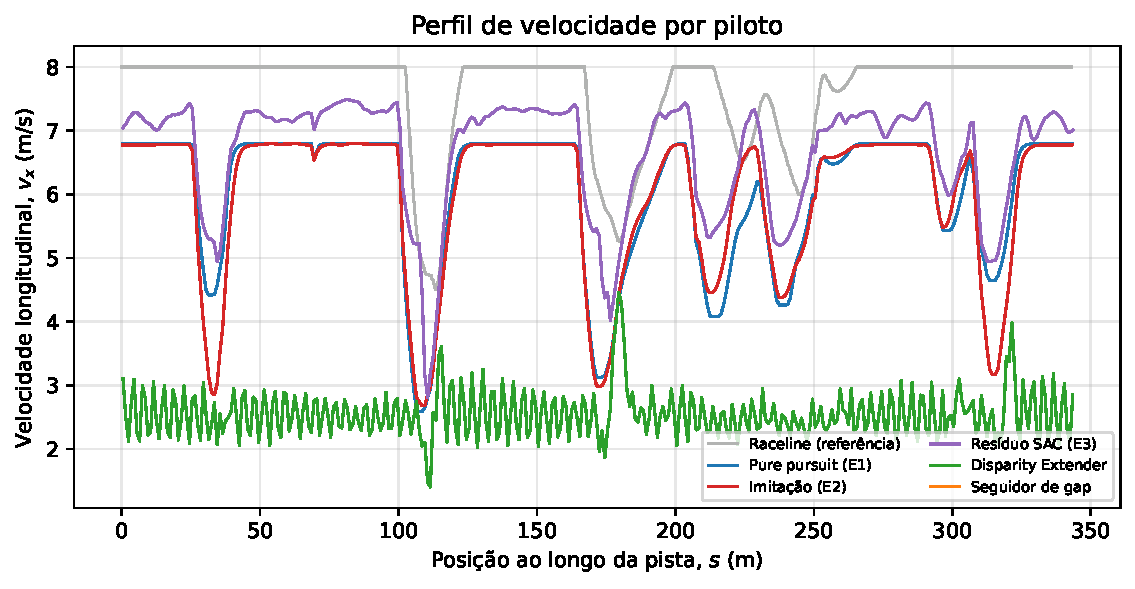
\includegraphics[width=\textwidth]{figs/comparativo/perfil_velocidade}
    \caption{Perfil de velocidade dos pilotos automáticos em Spielberg:
    velocidade longitudinal média por faixa de 1~m da posição $s$ ao longo da
    volta, sobre as voltas completas. A curva cinza é a velocidade de referência
    da linha de corrida}
    \label{fig:cmp_perfil}
\end{figure}

A Figura~\ref{fig:cmp_esterco} põe cada volta completa num plano de taxa de
esterço contra tempo de volta. Os pilotos formam grupos separados, sem
sobreposição entre eles exceto a do E1 com o E2. Não há relação monotônica entre
as duas grandezas: o piloto mais rápido, o E3, esterça mais que o E1 e o E2, e o
mais lento, o Disparity Extender, é também o que mais esterça.

\begin{figure}[htb]
    \centering
    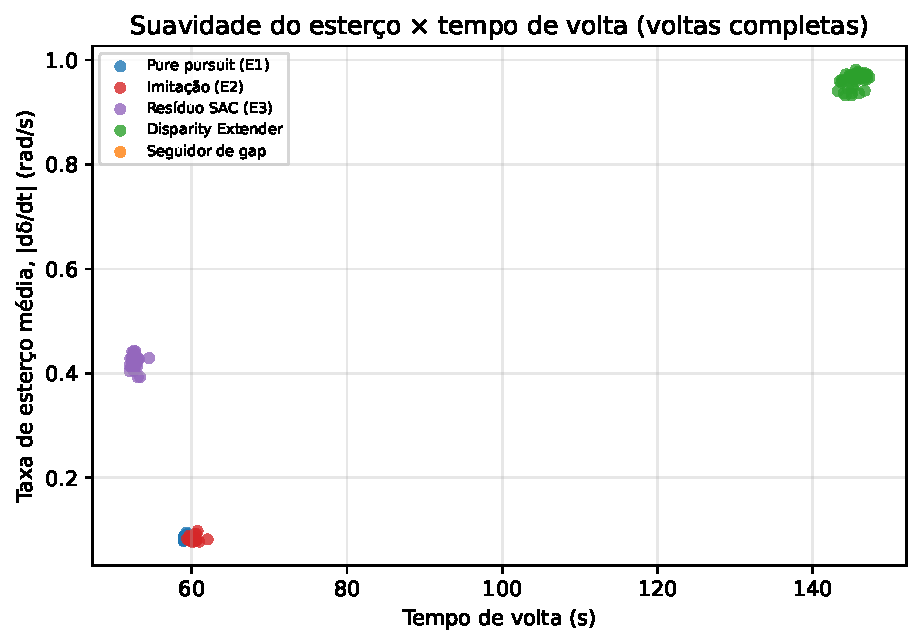
\includegraphics[width=0.85\textwidth]{figs/comparativo/esterco_vs_tempo}
    \caption{Taxa média de esterço contra tempo de volta, uma marca por volta
    completa de cada piloto automático}
    \label{fig:cmp_esterco}
\end{figure}

A Figura~\ref{fig:cmp_trajetorias} mostra, no trecho de maior curvatura da linha
de corrida, a trajetória da volta de tempo mediano de cada piloto. As
trajetórias do E1, do E2 e do E3 praticamente se sobrepõem e acompanham a linha
de corrida de perto. A do Disparity Extender ondula de um lado a outro do
corredor, inclusive na reta de saída, o que é a forma geométrica da sua taxa de
esterço e do seu desvio.

\begin{figure}[htb]
    \centering
    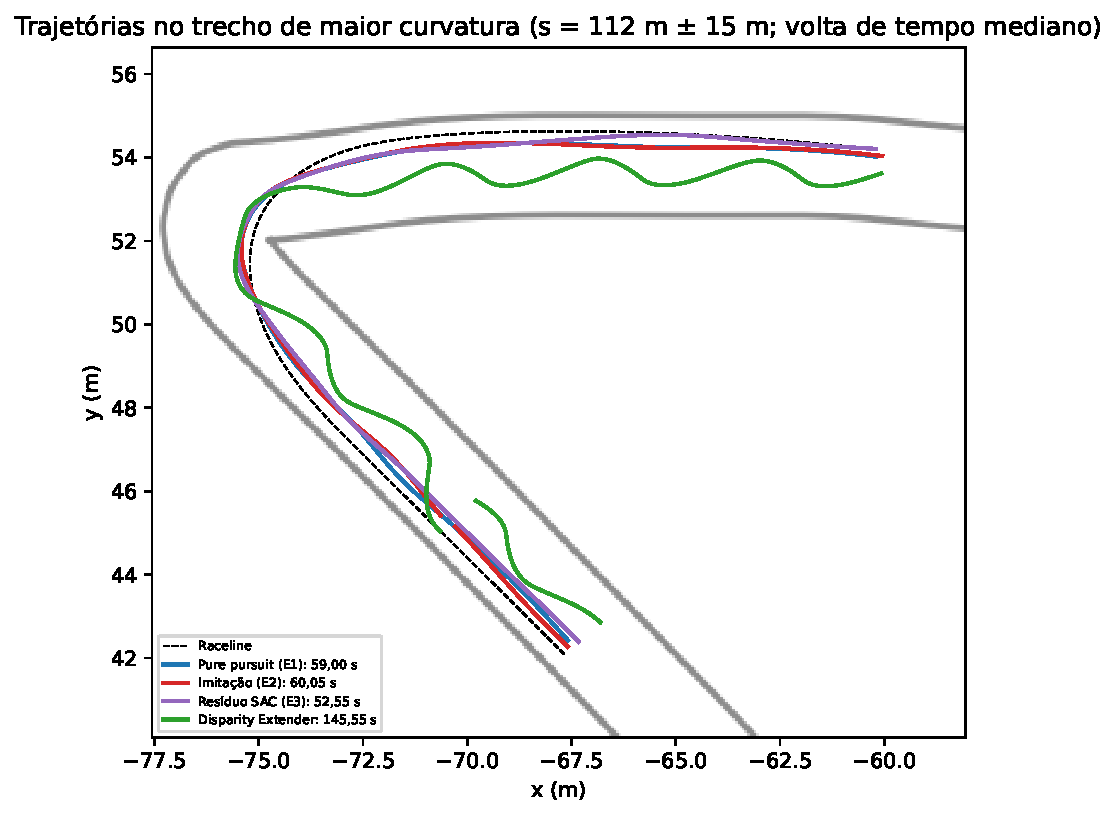
\includegraphics[width=0.85\textwidth]{figs/comparativo/trajetorias_curva}
    \caption{Trajetórias da volta de tempo mediano de cada piloto automático no
    trecho de maior curvatura da linha de corrida de Spielberg, com 15~m para
    cada lado do ponto de maior curvatura. A linha tracejada é a linha de
    corrida. A trajetória do Disparity Extender aparece em dois trechos porque a
    largada sorteada daquela volta caiu dentro da janela: o início e o fim da
    volta passam pelo trecho em momentos diferentes e não se ligam}
    \label{fig:cmp_trajetorias}
\end{figure}

\subsection{Pilotos humanos}\label{sec:res-cmp-humanos}

As sessões humanas seguem o protocolo da Seção~\ref{sec:val-humano}: em cada
vista, dez minutos de treino e três sessões de cinco voltas nas sementes 1000,
1001 e 1002, primeiro com a pista inteira e depois só com o LiDAR. As linhas
humanas da Tabela~\ref{tab:comparativo} estão reservadas e ainda vazias.
Participaram \pendentehumano{número de autores e de voluntários, por grupo e
experiência em jogos de corrida; sessões excluídas e motivo}.

\textbf{Resultado por piloto e vista.} Na vista da pista inteira, os pilotos
humanos completaram \pendentehumano{voltas completas/tentadas, colisões, mediana
e melhor volta, por piloto, autores separados dos voluntários}. Na vista só
LiDAR, \pendentehumano{os mesmos campos na vista só LiDAR}.

\textbf{Tempo real.} O passo de controle humano é segurado até 0,05~s de relógio
e o atraso de cada passo é registrado. Nas sessões que contam,
\pendentehumano{atraso médio, percentil 99 e passos fora do prazo, por sessão}.

A Figura~\ref{fig:cmp_curva} mostra o tempo de cada volta humana na ordem em que
foi feita, do treino às três sessões de cada vista.
\pendentehumano{leitura da curva de aprendizado: tendência no treino, diferença
entre a primeira e a terceira sessão e mudança na troca de vista}.

\begin{figure}[htb]
    \centering
    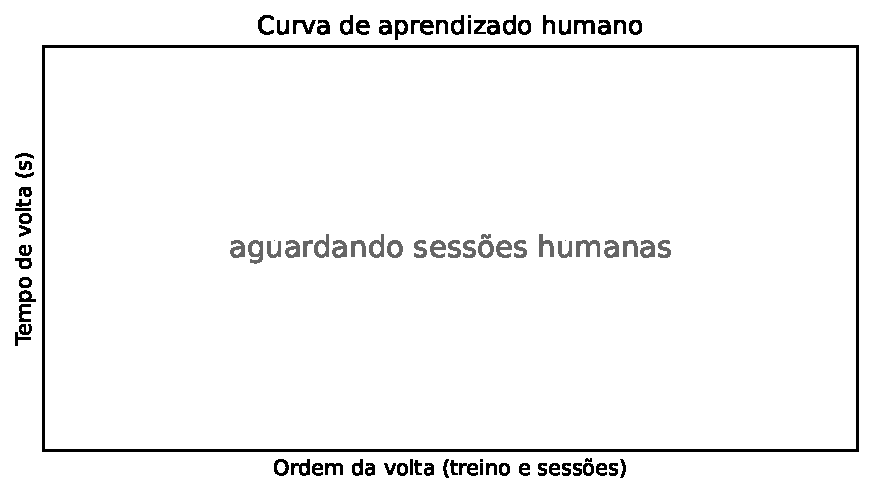
\includegraphics[width=0.85\textwidth]{figs/comparativo/curva_aprendizado}
    \caption{Curva de aprendizado dos pilotos humanos: tempo de volta na ordem
    cronológica, no treino e nas três sessões de cada vista}
    \label{fig:cmp_curva}
\end{figure}

\textbf{Faixa do grupo e posição das políticas.} Por vista, a faixa do grupo
humano --- melhor, mediana e pior piloto pela mediana de tempo de volta --- é
\pendentehumano{faixa do grupo na vista da pista inteira e na vista só LiDAR, e
posição de E1, E2, E3 e Disparity Extender em relação a ela}.

\textbf{Comparação entre as vistas.} Com a mesma pessoa nas duas vistas,
\pendentehumano{diferença de conclusão e de tempo de volta entre a pista inteira
e só o LiDAR, por piloto}. Como a ordem das vistas é fixa, essa diferença mistura
o efeito da informação com o da prática acumulada.

\section{Discussão}\label{sec:res-discussao}

\subsection{O que os números sustentam}

A Tabela~\ref{tab:res_sintese} reúne as etapas da cascata e os demais pilotos
do comparativo na comparação que organiza o argumento do trabalho: desempenho
contra dependência de infraestrutura de percepção. As colunas oficiais são as
dos portões; as do comparativo, as da Seção~\ref{sec:res-comparativo}.

\begin{table}[htb]
    \centering
    \footnotesize
    \setlength{\tabcolsep}{2.5pt}
    \begin{tabular}{|l|c|c|c|c|c|c|c|}
        \hline
        & & \multicolumn{3}{c|}{\textbf{Portão oficial}} &
        \multicolumn{2}{c|}{\textbf{Comparativo}} & \\
        \cline{3-7}
        \textbf{Piloto} & \textbf{Tipo} & \textbf{Volta (s)} &
        \textbf{Razão a $T_{pp}$} & \textbf{Concl.} & \textbf{Volta (s)} &
        \textbf{Concl.} & \textbf{Pose global?} \\
        \hline
        E1 (\textit{pure pursuit}) & clássico & 59,000 & 1,000 & 50/50 & 59,00 &
        44/45 & sim \\
        \hline
        E2 (TinyLidarNet) & ML & 60,050 & 1,018 & 50/50 & 60,05 & 50/50 & não \\
        \hline
        E3 (E2 + resíduo SAC) & ML & 52,525 & 0,890 & 91/92 & 52,55 & 50/50 & não \\
        \hline
        Disparity Extender & clássico & --- & --- & --- & 145,55 & 50/50 & não \\
        \hline
        Seguidor de gap & clássico & --- & --- & --- & --- & 0/5 & não \\
        \hline
        Humano, pista inteira & humano &
        \multicolumn{5}{c|}{\pendentehumano{faixa do grupo}} & vê o mapa \\
        \hline
        Humano, só LiDAR & humano &
        \multicolumn{5}{c|}{\pendentehumano{faixa do grupo}} & não \\
        \hline
    \end{tabular}
    \caption{Síntese dos pilotos em Spielberg. As colunas oficiais são as dos
    portões: o E1 sem randomização, o E2 e o E3 com ela. As colunas do
    comparativo são todas com randomização, cinco sementes de dez voltas;
    a volta é a mediana sobre as voltas completas. Nas linhas humanas, a faixa é
    a do grupo (melhor, mediana e pior piloto)}
    \label{tab:res_sintese}
\end{table}

A cascata faz o que se propôs a fazer. A destilação transfere a competência do
especialista para uma política que enxerga apenas LiDAR e proprioceptiva, ao
custo medido de 1,8\% de tempo de volta; o resíduo recupera esse custo e
\textbf{ultrapassa a política ensinante em 11,0\%}, sem devolver a dependência de
localização, e mantendo a taxa de conclusão acima de 0,98 e a degradação sob
randomização de atrito em zero. Fora do circuito de coleta, a rede destilada
supera o especialista de forma mais dramática ainda, completando voltas em duas
pistas onde o professor completa 16,7\% e 0\%.

Uma assimetria de protocolo favorece a leitura conservadora e vale declará-la. O
denominador $T_{pp}$ é medido \textbf{sem} randomização, enquanto os numeradores
das etapas E2 e E3 são medidos \textbf{com} randomização de atrito, de posição de
largada e de ruído de sensor. A vantagem de 11,0\% do resíduo é, portanto, obtida
por uma política avaliada em condições mais duras que a referência que ela supera.
O braço sem randomização da comparação pareada da etapa E3 permite estimar o
tamanho desse efeito: 52,500~s contra 52,600~s, isto é, cerca de um décimo de
segundo. A assimetria existe, é declarada, e é pequena --- mas ela existe, e um
leitor que compare 52,525~s com 59,000~s deve saber que os dois números não foram
medidos sob o mesmo protocolo.

O comparativo permite fazer essa comparação sob o mesmo protocolo, sem trocar o
número oficial. Com randomização, nas mesmas cinco sementes, o especialista
mediu 59,00~s e o resíduo 52,55~s: a ordem e a distância entre os dois se mantêm,
e a mediana do especialista não se moveu com a randomização. O que a
randomização acrescentou ao especialista foi uma colisão em 45 voltas, e não
tempo de volta.

\subsection{Primeira ressalva: o limiar cai dentro do intervalo de confiança}\label{sec:res-ic}

Nos três portões aprovados, o intervalo de Wilson reportado ao lado da taxa de
conclusão \textbf{contém o limiar}. A Tabela~\ref{tab:val_ic} registra os três
casos, e a Seção~\ref{sec:val-limitacoes} discute a decisão pré-registrada que
leva a isso e quantifica por que o limite inferior do intervalo não pôde ser o
critério nesta escala de amostra. Não se repete aqui essa justificativa; o que
cabe é medir o seu efeito sobre os resultados que este capítulo acabou de
reportar.

O efeito é este: \textbf{se o critério fosse o limite inferior do intervalo, as
três etapas reprovariam} --- a etapa E1 com 0,9287 contra limiar 1,00, a etapa E2
com 0,9287 contra 0,95 e a etapa E3 com 0,9410 contra 0,98. Nenhum dos três
resultados sobreviveria, inclusive os dois que não cometeram uma única falha em
50 voltas. A ressalva não é, portanto, uma sombra sobre um dos portões: ela é
constitutiva de todos eles, e a única forma de removê-la seria medir mais voltas
por configuração avaliada, não escrever o critério de outro jeito.

Convém delimitar o que ela alcança, com os artefatos deste capítulo. Ela alcança
o critério de taxa de conclusão e nenhum outro: os dois critérios de robustez a
atrito da etapa E3 estão a mais de uma ordem de grandeza dos seus limiares, e os
intervalos BCa de tempo de volta ficam inteiramente abaixo dos limiares em E2 e
E3.

O que ela \textit{não} respeita é a fronteira entre aprovar e reprovar, e seria
cômodo supor o contrário --- que uma reprovação, por ser negativa, esteja a salvo
da ressalva que atinge a aprovação. Os artefatos dizem o oposto. Dos quatro
pontos medidos do E3, \textbf{três têm o limiar de 0,98 dentro do intervalo de
Wilson}: os dois que passam no critério de taxa de conclusão e um dos dois que
reprovam nele, como a Seção~\ref{sec:res-e3} abre. Só a reprovação do ponto de 300 mil passos sem
penalidade de proximidade é robusta à escolha de critério, e é a única. Nos
outros três, inclusive na aprovação que é o resultado final do trabalho, a
decisão repousa inteiramente sobre o valor pontual.

Não há como transformar isso numa boa notícia, e a conduta que a
Seção~\ref{sec:val-limitacoes} adota permanece a única defensável. É também a
razão de este capítulo imprimir os quatro intervalos do E3 em vez de só as
quatro taxas: sem eles, o fato de a configuração aprovada e a anterior não se
separarem por intervalo não apareceria em lugar nenhum do trabalho.

\subsection{Segunda ressalva: a realização não é a distribuição}

A segunda ressalva é mais severa que a primeira e atinge especificamente a etapa
E3. A Tabela~\ref{tab:val_sensibilidade} mede a sensibilidade das duas políticas
a perturbação numérica irrelevante, e a Seção~\ref{sec:val-limitacoes} analisa o
que ela implica: a amplitude é de \textbf{0,0381} para a política composta e
\textbf{nula} para a rede de imitação isolada.

O que este capítulo acrescenta é a confrontação dessa amplitude com as margens
que ele acabou de reportar. A margem da etapa E3 sobre o seu limiar é
$0{,}9891 - 0{,}98 = 0{,}0091$; a amplitude sob perturbação irrelevante é
0,0381, \textbf{mais de quatro vezes maior}. A margem da etapa E2 sobre o seu
limiar é 0,05, contra amplitude nula. Em outras palavras: a aprovação da etapa E2
é robusta à realização numérica da política, e a da etapa E3 não é.

A consequência precisa ser dita sem atenuação. \textbf{Para a etapa E3, o número
reproduzível é a distribuição, não a realização.} Quem reimplementar a
composição com outra ordem de operações, outro tipo de ponto flutuante ou outra
versão da biblioteca de álgebra medirá outro valor dessa faixa, e esse valor
pode ficar abaixo do limiar. O 0,9891 da Tabela~\ref{tab:res_e3_criterios} é uma
realização legítima, medida com a composição única que o contrato numérico
determina, num artefato com proveniência íntegra --- e não é um valor que se deva
esperar reproduzir dígito a dígito noutra implementação.

Duas qualificações fecham o ponto. A primeira é de escopo, e coincide com a da
ressalva anterior por um motivo diferente: como a perturbação reembaralha
\textit{qual} episódio termina em colisão sem deslocar o resultado numa direção,
ela atinge a contagem de voltas e não o tempo de volta, cuja mediana no E3 tem
intervalo BCa de apenas 0,21~s de largura. A segunda é mais incômoda: o estudo de
sensibilidade foi feito na máquina anterior do projeto, cujas execuções não
sobreviveram à migração --- fato declarado na Seção~\ref{sec:val-limitacoes}. A
confrontação entre margem e amplitude que esta subseção faz combina, portanto, um
número auditável nesta máquina com uma amplitude medida numa execução que já não
é reconferível. Reproduzir o estudo neste host é a forma de fechar a lacuna, e
não foi feito.

\subsection{Terceira ressalva: a sobreposição do conjunto de generalização}

A sobreposição entre o conjunto de coleta e o conjunto de generalização foi
tratada duas vezes: a Seção~\ref{sec:val-heldout} expõe o defeito de desenho que
a produz, mostra por que ele era mais grave para execuções futuras do que para a
execução reportada, explica por que a correção não pôde ser aplicada
retroativamente e registra a regra que a fechou para as execuções seguintes; a Seção~\ref{sec:res-e2} deste capítulo acrescenta a metade
recíproca, que a mesma coleta foi causalmente necessária.

O que resta dizer, e é a consequência prática para quem lê os números, cabe em
duas linhas. \textbf{Nenhum valor deste capítulo deve ser citado como
``generalização em três pistas não vistas''}: das três pistas que pontuam o
critério, apenas Oschersleben é inteiramente inédita. E o valor de generalização
do E3 simplesmente não existe --- o resíduo nunca foi avaliado fora de
Spielberg, o que é o segundo item da lista da subseção seguinte, e não uma
variante desta ressalva.

\subsection{O que os números não sustentam}

Além das três ressalvas acima, seis limites delimitam o alcance dos resultados
deste capítulo. Nenhum deles é atenuado.

\begin{itemize}
    \item \textbf{Uma execução por configuração.} Os quatro pontos da
          Tabela~\ref{tab:res_e3_pontos} diferem por uma variável cada, mas cada
          ponto é \textit{um} treino. A variabilidade entre sementes de
          \textbf{treino} não foi medida em nenhuma etapa --- as 5 ou 10
          sementes dos portões são de \textbf{avaliação}, sobre um ponto de
          verificação fixo. A diferença entre as duas últimas configurações ---
          três colisões contra uma --- é atribuída à penalidade de proximidade
          porque foi a única variável alterada, mas o trabalho não mediu quanto
          dessa diferença caberia dentro da dispersão de dois treinos com a
          mesma configuração e sementes distintas. Essa é a lacuna mais direta a
          fechar.
    \item \textbf{Um circuito de portão.} Todos os critérios de aceite das três
          etapas são medidos em Spielberg. As outras quatro pistas entram apenas
          no critério de generalização da etapa E2, e nenhuma delas pontua a
          etapa E3: o resíduo não foi avaliado fora do circuito em que treinou.
    \item \textbf{Um simulador e um modelo de veículo.} A fidelidade do modelo
          de faixa única é premissa herdada, e a Seção~\ref{sec:val-colisao}
          registra que o detector de colisão do simulador precisou ser corrigido
          antes que qualquer número deste capítulo fosse reportável --- o que é
          evidência a favor da desconfiança, não contra ela.
    \item \textbf{Veículo único, sem corrida direta.} Não há ultrapassagem, nem
          oponente, nem obstáculo dinâmico, pelos motivos que a
          Seção~\ref{sec:arte-lacuna} declara.
    \item \textbf{Nenhum resultado fora da simulação.} Toda comparação
          numérica deste capítulo com resultados de campo da literatura é
          assimétrica, e assim deve ser lida.
    \item \textbf{A evidência não é durável.} Os relatórios que sustentam cada
          número deste capítulo não são versionados, e o relatório de
          verificação é sobrescrito a cada execução, de modo que medições
          feitas por esse relatório não podem ser reconferidas depois. No
          comparativo, o resumo das execuções --- tabela, figuras, dados
          agregados e registros das varreduras --- está versionado junto com
          este texto, mas os dados passo a passo, não.
\end{itemize}

\subsection{O comparativo: controladores clássicos e de aprendizado de máquina}\label{sec:res-disc-cmp}

\textbf{Mesma informação, desempenhos distintos.} Quatro pilotos do comparativo
executam apenas com LiDAR e proprioceptiva: o E2, o E3 e os dois reativos. Sob o
mesmo protocolo, os dois aprendidos completam 50 de 50 voltas em 60,05~s e
52,55~s; o Disparity Extender completa 50 de 50 em 145,55~s; e o seguidor de gap
não completa volta. O único piloto que usa pose global e linha de corrida, o
E1, fica em 59,00~s. Com o mesmo sensor em execução, as políticas aprendidas
chegaram ao tempo do piloto que usa o mapa, e uma delas o superou; os
controladores reativos, não.

\textbf{O que essa comparação não diz.} Ela compara estas implementações, e não
as famílias de método. Três diferenças entre os dois lados precisam acompanhar
os números. Os reativos são portes de nós escritos para um veículo real lento,
ajustados por uma varredura de no máximo 24 combinações por grade (48 no
seguidor de gap, que teve duas grades), e a configuração do
Disparity Extender ficou no limite da sua grade. Os aprendidos passaram por laços
automáticos com várias tentativas e ações pré-declaradas (Seções~\ref{sec:res-e2}
e~\ref{sec:res-e3}). E, sobretudo, os aprendidos foram treinados com
demonstrações de um especialista que usa pose e linha de corrida: eles não
precisam do mapa em execução, mas a informação do mapa de Spielberg entrou neles
pelo treino. Os reativos não têm acesso a essa informação em momento algum. A
vantagem que eles teriam --- funcionar num circuito desconhecido, sem mapa e sem
treino, como argumenta a Seção~\ref{sec:arte-classico} --- não é medida aqui,
porque o comparativo usa uma só pista.

\textbf{Suavidade e desvio.} O E1 e o E2 têm a mesma taxa de esterço,
0,08~rad/s; o E3, o mais rápido, sobe para 0,42~rad/s;
o Disparity Extender tem a maior taxa, 0,97~rad/s, e o maior tempo. A taxa de
esterço, sozinha, não ordena os pilotos por desempenho, e a
Figura~\ref{fig:cmp_esterco} mostra que não há relação monotônica entre as duas
grandezas. O desvio da linha de corrida também não é medida de qualidade: o E3
se afasta mais dela que o E1 e o E2 (0,40~m em média, contra 0,26 e 0,27~m) e é o
mais rápido. O que o desvio mede é a semelhança com o especialista, cuja
referência é a própria linha de corrida.

\textbf{Por que o seguidor de gap não completa volta.} Os dados das varreduras
são compatíveis com dois mecanismos, que se somam. O primeiro está na escolha do
alvo. A detecção por descontinuidade define uma abertura por um salto de alcance
maior que o limiar de profundidade entre pontos consecutivos do \textit{scan}.
Numa pista fechada e sem obstáculos, as paredes produzem um \textit{scan}
contínuo, exceto onde uma parede próxima esconde um trecho mais distante, o que
ocorre tipicamente na borda interna de uma curva. As bordas das aberturas
candidatas caem, assim, sobre a própria parede, e o alvo, pontuado por distância e
largura, fica junto a uma dessas bordas, e não no centro do corredor livre. O
Disparity Extender, ao contrário, estende cada disparidade pela largura do carro
antes de escolher, o que afasta o alvo da borda. O segundo mecanismo é a
oscilação do esterço. Com ganho proporcional de 1,5 ou 2,2, a taxa média de
esterço por combinação da grade oficial ficou entre 0,41 e 1,98~rad/s, contra
0,08~rad/s do E1, o que é compatível com um esterço que oscila entre os limites:
com o atraso de dois passos (100~ms), o PID corrige um erro que o carro já deixou
para trás, e um ganho alto transforma essa defasagem em oscilação. A isso se soma
a saturação: o nó original permitia 0,7~rad de esterço, e o porte corta em
0,4189~rad, como todos os pilotos.

A grade ampliada separa os dois mecanismos, e é por isso que ela é informativa
apesar de não ter produzido volta. Com ganho de 0,3, a taxa média de esterço,
medida como média do episódio de sonda, caiu para 0,08 a 0,29~rad/s, e, com a
velocidade comandada pelo PID, para 0,08 a 0,11~rad/s, perto dos 0,08~rad/s do E1
e do E2 (na tabela, essa grandeza é a mediana, entre voltas completas, da média
de cada volta, de modo que a comparação é de ordem de grandeza), e o carro
continuou batendo
nos primeiros metros, com progresso médio de no máximo 8,20~m. Um esterço suave
não bastou, o que aponta a escolha do alvo como causa dominante --- e a escolha do
alvo não depende de nenhum dos parâmetros varridos. Esta é uma interpretação de
dados agregados: o alvo escolhido a cada passo não foi gravado, e confirmá-la
exigiria gravá-lo. O que não depende de interpretação é o resultado, obtido pelo
critério fixado antes da medição: o seguidor de gap, nesta implementação e neste
regime de velocidade e atraso, não completa uma volta em Spielberg.

\textbf{A comparação com os pilotos humanos.} O desenho é descritivo e não tem
teste de hipótese (Seção~\ref{sec:val-humano}). O que ele permite dizer é a
posição de cada política em relação à faixa do grupo humano, vista a vista, e a
leitura de cada vista foi fixada antes da coleta. Na vista só LiDAR, humanos e
políticas sem pose recebem informação equivalente --- o \textit{scan} atual,
dentro de um alcance fixo, e a velocidade no painel ---, e a diferença entre eles é de
decisão e de controle; na vista da pista inteira, o humano vê o mapa e pode
antecipar as curvas, e a diferença mistura habilidade com informação. Com os
dados, \pendentehumano{posição de E1, E2, E3 e Disparity Extender em relação à
faixa do grupo, por vista}.

Dois cruzamentos têm leitura direta. O primeiro é entre o humano na vista só
LiDAR e o seguidor de gap, que reagem ao mesmo \textit{scan} do passo atual:
\pendentehumano{se e quanto os humanos na vista só LiDAR completaram as voltas que
o seguidor de gap não completa}. O segundo é a suavidade:
\pendentehumano{taxa de esterço e desvio da linha de corrida dos humanos diante
das políticas}. Das limitações da Seção~\ref{sec:val-limitacoes-comparativo},
cinco acompanham qualquer uma dessas leituras: a informação desigual na vista da
pista inteira, a ordem fixa das vistas, a amostra pequena, a separação entre
autores e voluntários e a pista única.


\subsection{Síntese}

O resultado quantitativo do trabalho é uma política que enxerga apenas LiDAR e
proprioceptiva, completa 91 de 92 voltas sob randomização de atrito, posição de
largada e ruído de sensor, e percorre o circuito em 52,525~s --- 11,0\% mais
rápido que o especialista geométrico que originou os seus rótulos e que depende
de pose global para funcionar. A cascata de três etapas preserva, em cada passo,
a propriedade conquistada no anterior: o especialista fornece competência, a
imitação a transfere para uma política sem pose global, e o resíduo recupera e supera
o desempenho perdido na destilação sem devolver a dependência de localização, com
o pior caso da terceira etapa sendo o resultado da segunda.

Sob o protocolo comum do comparativo, a ordem se mantém: com randomização e nas
mesmas cinco sementes, o resíduo faz 52,55~s, o especialista 59,00~s e a rede de
imitação 60,05~s. Dos dois controladores reativos que usam apenas o LiDAR, o
Disparity Extender completa todas as voltas em 145,55~s, e o seguidor de gap não
completa nenhuma, nem nas 48 combinações das duas varreduras nem na avaliação
congelada. Quanto aos pilotos humanos, \pendentehumano{uma frase com a posição das
políticas diante da faixa do grupo humano em cada vista}.

O resultado metodológico é de outra natureza e, no julgamento deste trabalho, é o
mais transferível dos dois. As três ressalvas discutidas acima --- o limiar dentro
do intervalo, a sensibilidade da política composta a perturbação irrelevante, e a
sobreposição entre o conjunto de generalização e as ações de correção --- não
foram descobertas por um revisor depois do resultado. Duas delas estavam
declaradas, com o motivo quantificado, \textbf{antes} de qualquer medição, e a
terceira foi encontrada conferindo o artefato contra o texto que o descrevia, e
declarada em vez de corrigida retroativamente, porque corrigi-la depois de ver o
número seria o defeito maior. Um capítulo de resultados que apresentasse apenas os
valores da Tabela~\ref{tab:res_sintese} teria omitido o que este trabalho de fato
tem de incomum: não os números, mas a possibilidade de dizer com precisão o que
eles não sustentam.

% ----------------------------------------------------------
% Conclusão e Trabalhos Futuros
% Capítulo sem numeração, mas presente no Sumário
% ----------------------------------------------------------

\chapter*[Conclusão e Trabalhos Futuros]{Conclusão e Trabalhos Futuros}\label{cap:conclusao}
\addcontentsline{toc}{chapter}{Conclusão e Trabalhos Futuros}

Este trabalho se propôs a comparar, num mesmo simulador da plataforma F1TENTH e
sob os mesmos critérios de avaliação, três formas de pilotar um veículo de
corrida em escala 1:10: controladores clássicos, políticas obtidas por
aprendizado de máquina e pilotos humanos. O que ele entrega e o que ele não
entrega separam-se por uma fronteira nítida, e é ela que organiza esta
conclusão. Estão medidos, em simulação e sob um protocolo comum, os cinco pilotos
automáticos: o \textit{pure pursuit} do E1, o Disparity Extender e o seguidor de
gap por descontinuidade, do lado clássico, e a rede de imitação do E2 e o resíduo
de aprendizado por reforço do E3, do lado do aprendizado de máquina. Estão
prontos a interface de pilotagem humana e o protocolo da coleta. Faltam as
sessões com os pilotos humanos, e cada ponto desta conclusão que depende delas
está marcado como pendente.

Esta conclusão retoma do Capítulo~\ref{cap:resultados} apenas os números que
sustentam as suas afirmações e não reconstrói o argumento do
Capítulo~\ref{cap:metodologia}. Ela faz duas coisas:
enuncia o que o trabalho sustenta e responde um a um aos quatro objetivos
específicos declarados na seção \textit{Objetivos} da Introdução.

\section*{Conclusões}
\addcontentsline{toc}{section}{Conclusões}

\subsection*{O que o trabalho mediu}

A cascata de três etapas cumpriu, em simulação, o que se propôs a fazer, e a
Tabela~\ref{tab:res_sintese} do Capítulo~\ref{cap:resultados} a resume numa linha
por piloto, ao lado dos demais pilotos do comparativo. O especialista geométrico da etapa E1 fixou o tempo de referência
$T_{pp} = 59{,}000$~s, com 50 de 50 voltas sem colisão e com determinismo
verificado --- o valor reproduziu dígito a dígito uma medição anterior feita em
outra arquitetura, o que é o que autoriza usá-lo como denominador de todos os
critérios seguintes. A rede de imitação da etapa E2 aprovou os quatro critérios
do seu portão e pagou 1,8\% de tempo de volta pela troca que define o trabalho:
deixar de exigir pose global. E o resíduo de aprendizado por reforço da etapa E3
aprovou os seus quatro critérios completando 91 de 92 voltas sob randomização e
percorrendo o circuito em 52,525~s, \textbf{11,0\% mais rápido que o especialista
que originou os seus rótulos}, sem devolver a dependência de localização e com
degradação desprezível sob randomização do coeficiente de atrito --- queda de
taxa de conclusão nula, e piora de tempo de volta de 0,0019 contra um limiar de
0,05.

As três ressalvas que o Capítulo~\ref{cap:resultados} discute nominalmente
acompanham esses números e não são atenuadas em lugar nenhum do texto: o limiar
de taxa de conclusão cai dentro do intervalo de confiança nos três
portões aprovados (Tabela~\ref{tab:val_ic}); a política composta da etapa E3 é
sensível a perturbação numérica irrelevante numa amplitude quatro vezes maior que
a sua margem sobre o limiar, de modo que o número reproduzível ali é a
distribuição e não a realização (Tabela~\ref{tab:val_sensibilidade}); e duas das
quatro pistas do critério de generalização da etapa E2 haviam entrado no conjunto
de coleta, o que dilui aquele critério em vez de inflá-lo
(Seção~\ref{sec:val-heldout}). Duas dessas três estavam declaradas, com o motivo
quantificado, antes de qualquer medição; a terceira foi encontrada conferindo o
artefato contra o texto que o descrevia, e foi declarada em vez de corrigida
retroativamente.

Uma outra ressalva, declarada nos mesmos capítulos fora da lista das três, é de \textbf{protocolo}: o
denominador $T_{pp}$ é medido \textbf{sem} randomização, enquanto as etapas E2 e
E3 são medidas \textbf{com} randomização de atrito, de posição de largada e de
ruído de sensor. A comparação entre 52,525~s e 59,000~s não é, portanto, entre
medições feitas sob o mesmo protocolo. A direção do efeito favorece a leitura
conservadora --- a política que supera a referência é a que corre em condições
mais duras, e o braço sem randomização da comparação pareada da etapa E3 estima o
tamanho disso em cerca de um décimo de segundo ---, mas o padrão deste trabalho é
declarar a assimetria, não confiar na direção dela. O comparativo a mede
diretamente: com randomização e nas mesmas sementes, o especialista fez 59,00~s, e
o resíduo, 52,55~s.

\subsection*{O que o comparativo mediu}

Sob o protocolo comum, os pilotos automáticos se separam em três grupos. Os
pilotos aprendidos e o especialista completam a volta entre 52,55~s e 60,05~s: o
resíduo em 52,55~s, o especialista em 59,00~s, com uma colisão em 45 voltas, e a
rede de imitação em 60,05~s, com taxa de esterço e desvio da linha de corrida
praticamente iguais aos do especialista que ela imita. O Disparity Extender
completa todas as 50 voltas, mas em 145,55~s, com a maior taxa de esterço e o
maior desvio da linha de corrida. E o seguidor de gap não completa volta alguma:
nenhuma das 48 combinações das duas varreduras de parâmetros completou uma volta
de sonda, e a configuração congelada colidiu nas cinco sementes da avaliação. Com
o mesmo sensor em execução, as políticas aprendidas alcançaram o piloto que usa
a pose e a linha de corrida calculada sobre o mapa, o E1; os controladores
reativos, que não usam mapa, não. A ressalva central dessa leitura está na
Seção~\ref{sec:res-disc-cmp}: as políticas aprendidas não usam o mapa em
execução, mas a informação dele entrou no treino, pelas demonstrações do
especialista.

\subsection*{A contribuição metodológica}

O resultado que este trabalho considera mais transferível não é o tempo de volta.
É o aparato descrito no Capítulo~\ref{cap:metodologia}: um contrato numérico de
118 asserções com identificador estável, cada uma registrando a falha medida que a
originou; cinco camadas de verificação que vão da cobertura do contrato até a
proveniência do repositório; critérios de
aceite congelados no nascimento de cada execução, com a proveniência tratada como
parte do veredito e não como metadado; e uma tabela de ações de correção
pré-declaradas por critério, que é o que separa um experimento de uma busca
livre.

Nada disso é caro em si, e é essa a razão de o capítulo ser escrito como
argumento e não como manual. O que custa é a disciplina de aplicar cada regra
antes de a falha aparecer --- e a evidência oferecida é que, neste projeto, cada
uma delas foi escrita \textit{depois} de uma falha medida, cujo custo variou
entre uma tentativa de uma hora e oito execuções reprovadas em silêncio. Quatro
episódios sustentam o argumento inteiro: um detector de colisão que deixava o
veículo atravessar a parede e seguir dirigindo fora do circuito, um vazamento de
estado entre episódios que se disfarçava de má generalização, duas cópias da mesma
composição de política divergindo por um tipo numérico, e três valores distintos
para a mesma medição convivendo no repositório. Nos quatro, reexecutar o comando
devolvia o mesmo número; nos quatro, o número estava errado; e nos quatro a
distância até o valor correto era da mesma ordem das diferenças que o trabalho
pretendia demonstrar.

\subsection*{Os quatro objetivos, um a um}

A Introdução declarou quatro objetivos específicos. Dizer com precisão quais foram
atingidos, quais o foram em parte e quais não o foram é mais forte do que
dissolvê-los numa afirmação geral de êxito --- e é a única conduta compatível
com o Capítulo~\ref{cap:metodologia}, que argumenta o capítulo inteiro que
declarar o que não se cobre é parte do resultado. A
Tabela~\ref{tab:conc_objetivos} resume, e os parágrafos seguintes qualificam cada
linha.

\begin{table}[h]
    \centering
    \small
    \begin{tabularx}{\textwidth}{|c|>{\raggedright\arraybackslash}X|>{\raggedright\arraybackslash}p{3.3cm}|}
        \hline
        \textbf{\#} & \textbf{Objetivo específico declarado} & \textbf{Situação} \\
        \hline
        1 & Implementar e avaliar em simulação três controladores clássicos: o
        especialista \textit{pure pursuit}, que usa a linha de corrida calculada
        sobre o mapa, e dois reativos que usam apenas o LiDAR, o Disparity
        Extender e o seguidor de gap &
        atingido; o seguidor de gap não completa volta \\
        \hline
        2 & Treinar uma política de imitação sem pose global e refiná-la por
        aprendizado por reforço residual, sob critérios fixados antes da
        medição & atingido \\
        \hline
        3 & Desenvolver uma interface de pilotagem humana no mesmo simulador e
        coletar voltas de pilotos humanos sob protocolo fixado antes da coleta
        & em parte: interface e protocolo prontos, coleta pendente \\
        \hline
        4 & Comparar os três tipos de piloto quanto a conclusão de volta, tempo de
        volta, colisões, suavidade do esterço, desvio da raceline e perfil de
        velocidade, com o humano em duas condições de informação & em parte:
        pilotos automáticos comparados, humanos pendentes \\
        \hline
    \end{tabularx}
    \caption{Os quatro objetivos específicos declarados na Introdução diante do
    que o trabalho de fato mediu. A situação dos objetivos 3 e 4 é a desta
    versão, anterior às sessões humanas}
    \label{tab:conc_objetivos}
\end{table}

\textbf{Objetivo 1.} Os três controladores clássicos foram implementados e
avaliados sob o protocolo comum. O \textit{pure pursuit} tem dois números, que
convivem e não se substituem: o oficial, sem randomização, de 59,000~s e 50 de
50 voltas, que é o denominador $T_{pp}$ dos critérios de aceite; e o do
comparativo, com randomização, de 59,00~s e 44 de 45 voltas. O seguidor de gap foi
portado do nó ROS2 para o ambiente de pesquisa, passou pela varredura da grade
oficial e por uma grade ampliada criada depois dela, e foi avaliado na
configuração congelada: 0 de 5 voltas, com cinco colisões. O objetivo pedia
implementar e avaliar, e isso foi feito; o resultado da avaliação é negativo, e a
Seção~\ref{sec:res-disc-cmp} discute as causas prováveis. O Disparity Extender,
portado pelo mesmo caminho, completa 50 de 50 voltas em 145,55~s.

\textbf{Objetivo 2.} A rede de imitação sem pose global (E2) e o resíduo de
aprendizado por reforço (E3) foram treinados e avaliados sob portões cujos
limiares foram congelados antes da medição, e ambos aprovaram os seus critérios,
com as ressalvas declaradas acima (E2: 60,050~s e 50 de 50 voltas; E3: 52,525~s e
91 de 92 voltas, ambos com randomização). Reavaliados sob o protocolo comum, sem
retreino e já sob o avaliador corrigido, reproduziram as medianas a menos de
0,03~s (60,05~s e 52,55~s, ambos com 50 de 50 voltas).
A percepção consumida pela política é exclusivamente LiDAR bidimensional e
proprioceptiva, o que está declarado como limite na Seção~\ref{sec:arte-lacuna}.

\textbf{Objetivo 3.} A interface de pilotagem humana está pronta: \textit{joystick}
com os mesmos limites e o mesmo atraso das políticas, passo segurado em tempo
real com o atraso registrado, duas vistas e gravação no mesmo formato dos pilotos
automáticos (Seção~\ref{sec:prop-humano}). O protocolo da coleta está escrito,
com \textit{hash} gravado em cada registro (Seção~\ref{sec:val-humano}). A coleta
não foi feita: \pendentehumano{pilotos coletados (autores e voluntários), sessões
completas e excluídas, e a situação do Comitê de Ética}. A participação de
voluntários depende da resposta sobre a necessidade de submissão ao Comitê de
Ética em Pesquisa; sem ela, o estudo se limita aos autores.

\textbf{Objetivo 4.} A comparação entre os pilotos automáticos está feita, nas
seis métricas do objetivo, e a Tabela~\ref{tab:comparativo} já reserva as linhas
humanas. Falta a parte humana: \pendentehumano{faixa do grupo humano por vista e
posição de cada política em relação a ela}. Das limitações declaradas antes da
coleta (Seção~\ref{sec:val-limitacoes-comparativo}), cinco pesam diretamente
sobre essa parte: a informação desigual na vista da pista inteira, a ordem fixa
das vistas, a amostra pequena, a separação entre autores e voluntários e a pista
única.

\subsection*{O que fica dito com precisão}

Dos quatro objetivos, dois estão atingidos e dois em parte, e nenhum ficou sem
execução: os dois incompletos dependem da mesma coleta. O que o trabalho afirma,
nesta versão, é o que está medido: uma política que enxerga apenas LiDAR e
proprioceptiva completa 91 de 92 voltas sob randomização no seu portão e percorre
Spielberg 11,0\% mais rápido que o especialista geométrico que a ensinou; sob o
protocolo comum, ela faz 52,55~s contra 59,00~s do especialista, e os dois
controladores reativos que usam o mesmo sensor ficam muito atrás ou não
completam a volta. A afirmação sobre os humanos fica para depois da coleta:
\pendentehumano{afirmação central sobre humano e máquina, por vista}.

\section*{Trabalhos Futuros}
\addcontentsline{toc}{section}{Trabalhos Futuros}

Parte do que resta é continuação do próprio comparativo; parte são direções que a
literatura cobre e este trabalho deixa de fora.

\subsection*{As lacunas do próprio resultado em simulação}

A Seção~\ref{sec:res-discussao} lista sem atenuação o que os números não
sustentam. Cinco itens dali são acionáveis dentro do próprio simulador, e valem
como trabalho futuro imediato:

\begin{itemize}
    \item \textbf{Medir a variabilidade entre sementes de treino.} Cada
          configuração da etapa E3 corresponde a \textit{um} treino, e as
          sementes dos portões são de avaliação. Sem isso, não se sabe quanto da
          diferença entre a configuração aprovada e a anterior cabe dentro da
          dispersão de dois treinos idênticos. É a lacuna mais direta a fechar.
    \item \textbf{Avaliar o resíduo fora do circuito em que treinou.} Todos os
          critérios de aceite das três etapas são medidos em Spielberg, e a etapa
          E3 nunca foi pontuada em nenhuma outra pista: o valor de generalização
          do resíduo simplesmente não existe.
    \item \textbf{Reexecutar a etapa E2 sob a correção da sobreposição} entre o
          conjunto de coleta e o de generalização. A correção já está congelada
          no contrato (\texttt{SPEC-GATE-09}): nenhuma ação pré-declarada pode
          coletar numa pista de generalização. A
          Seção~\ref{sec:val-heldout} explica por que ela não podia ser
          aplicada retroativamente, e a execução reportada segue parcialmente
          contaminada até ser substituída.
    \item \textbf{Refazer o estudo de sensibilidade numérica nesta máquina.} As
          execuções que o sustentam são da máquina anterior do projeto e não
          sobreviveram à migração, de modo que a confrontação entre a margem da
          etapa E3 e a amplitude sob perturbação combina um número auditável com
          outro que já não é reconferível.
    \item \textbf{Tornar a evidência durável e completar o aparato.} Os
          relatórios das execuções oficiais não são versionados e o relatório
          de verificação é sobrescrito a cada execução; promovê-los para um
          caminho versionado, como já foi feito com os relatórios das cinco
          execuções do comparativo, torna toda medição reconferível. Os pontos
          de verificação das três etapas já foram medidos sob o avaliador
          corrigido, em que a colisão tem precedência sobre a chegada, no
          comparativo (Seção~\ref{sec:res-cmp-reavaliacao}); falta refazer sob
          ele os portões oficiais, com os seus critérios, e corrigir as poses de
          largada que nascem em colisão em Monza e Oschersleben, aceitando a
          perda de comparabilidade com as execuções anteriores.
\end{itemize}

\subsection*{Extensões do comparativo}

Do próprio comparativo, quatro extensões são diretas:

\begin{itemize}
    \item \textbf{Validação em hardware.} Todos os pilotos deste trabalho correm
          em simulação. Repetir o comparativo num veículo físico é a extensão de
          maior custo, e este trabalho não a aborda.
    \item \textbf{Imitação de pilotos humanos.} As voltas humanas gravadas passo a
          passo, no mesmo formato das demonstrações do especialista, podem servir
          de demonstração para a rede de imitação, no lugar do especialista
          geométrico.
    \item \textbf{Outras pistas.} O comparativo usa só Spielberg. Em pistas não
          vistas, a independência de mapa dos controladores reativos passa a
          contar, e a generalização das políticas aprendidas e dos humanos pode ser
          medida.
    \item \textbf{Contrabalanço das vistas.} A ordem fixa das vistas mistura o
          efeito da informação com o da prática. Alternar a ordem entre pilotos,
          com amostra maior, separa os dois.
\end{itemize}

Além dessas, permanecem em aberto as direções que a Seção~\ref{sec:arte-lacuna}
identifica como ausentes deste trabalho e presentes na literatura: corrida com
dois veículos e ultrapassagem, adaptação de modelo em linha, garantias formais
sobre a política e percepção além do LiDAR bidimensional.

\subsection*{Consideração final}

O trabalho termina com um comparativo em simulação cuja parte automática está
medida e cuja parte humana depende de coleta ainda por fazer. Sob o mesmo
protocolo, uma política que só vê o LiDAR, obtida por imitação de um especialista
geométrico e refinada por um resíduo de aprendizado por reforço, percorre
Spielberg mais rápido que esse especialista; o controlador reativo que usa o mesmo
sensor sem treino completa a volta em 145,55~s, e o outro não a completa. Onde os pilotos humanos se colocam diante disso,
\pendentehumano{uma frase com o resultado humano}. Dizer isso nessa ordem, com o
que está medido separado do que falta medir, é a mesma prática que o
Capítulo~\ref{cap:metodologia} defende como contribuição: declarar o que se
cobre, declarar o que não se cobre, e quantificar a distância entre os dois sempre
que houver medição que permita.


% ----------------------------------------------------------
% ELEMENTOS PÓS-TEXTUAIS (Referências, Glossário, Apêndices)
% ----------------------------------------------------------
\postextual

% Referências bibliográficas
% \makeatletter
% \let\bibstyle\@gobble
% \makeatother
\bibliography{bibliografia}

% Glossário (Consulte o manual)
%\glossary

% Apêndices
%% ----------------------------------------------------------
% Apêndices
% ----------------------------------------------------------

% ---
% Inicia os apêndices
% ---
\begin{apendicesenv}

% Imprime uma página indicando o início dos apêndices
\partapendices

% ----------------------------------------------------------
\chapter{Primeiro Apêncice}
% ----------------------------------------------------------

\lipsum[50] % Texto qualquer. REMOVER!!

% ----------------------------------------------------------
\chapter{Segundo apêndice com título tão grande quanto se queira porque ele já faz a quebra de linha da coisa toda}
% ----------------------------------------------------------
\lipsum[51-53] % Texto qualquer. REMOVER!!

\end{apendicesenv}
% ---

% Anexos
%% ----------------------------------------------------------
% Apêndices
% ----------------------------------------------------------

% ---
% Inicia os anexos
% ---
\begin{anexosenv}

% Imprime uma página indicando o início dos anexos
\partanexos

% ---
\chapter{Nome do Primeiro Anexo}
% ---
\lipsum[30] % Texto qualquer. REMOVER!!

% ---
\chapter{Nome de Outro Anexo}
% ---

\lipsum[32] % Texto qualquer. REMOVER!!

\end{anexosenv}

% Índice remissivo (Consultar manual)
%\phantompart
%\printindex

\end{document}
